\documentclass[a4paper,11pt]{book}

\usepackage{pgfgantt}
\usepackage{afterpage}
\usepackage{algorithm}
\usepackage{algpseudocode}
\usepackage{amsmath}
\usepackage[spanish,es-tabla]{babel}
\usepackage[backend=bibtex8, sorting=none]{biblatex}
\usepackage{booktabs}
\usepackage{colortbl, longtable}
\usepackage{dcolumn}
\usepackage{fancyhdr}
\usepackage{float}
\usepackage[stable]{footmisc}
\usepackage{graphicx}
\usepackage{hvfloat}
\usepackage[pdfborder={000}]{hyperref}
\usepackage[utf8]{inputenc}
\usepackage{listings}
\usepackage{longtable}
\usepackage{multirow}
\usepackage{pdfpages}
\usepackage{pgfgantt}
\usepackage{pgf-umlcd}
\usepackage{rotating}
\usepackage{url}
\usepackage{varwidth}
\usepackage{tocloft}
\usepackage{csvsimple}
\usepackage[spanish]{babel}
 \usepackage{capt-of}

\usepackage{xcolor}

\colorlet{punct}{red!60!black}
\definecolor{background}{HTML}{EEEEEE}
\definecolor{delim}{RGB}{20,105,176}
\colorlet{numb}{magenta!60!black}

\usetikzlibrary{babel}



\usepackage{siunitx}
\usepackage{tikz} % To generate the plot from csv
\usepackage{pgfplots}

\pgfplotsset{compat=newest} % Allows to place the legend below plot
\usepgfplotslibrary{units} % Allows to enter the units nicely

\sisetup{
	round-mode          = places,
	round-precision     = 2,
}

\decimalpoint
\newcolumntype{.}{D{.}{\esperiod}{-1}}
\makeatletter
\addto\shorthandsspanish{\let\esperiod\es@period@code}
\makeatother

\newenvironment{codigo}
 {\par\addvspace{\topsep}
  \centering
  \begin{minipage}{\linewidth}
  \hrule\kern2pt}
 {\par\kern2pt\hrule
  \end{minipage}
  \par\addvspace{\topsep}}

\RequirePackage{verbatim}



\newcommand{\myTitle}{Análisis y monitorización de aplicaciones a través de plugins con Naemon\xspace}
\newcommand{\myDegree}{Grado en Ingeniería Informática\xspace}
\newcommand{\myName}{Sofía Fernández Moreno\xspace}
\newcommand{\myProf}{Alberto Guillén Perales\xspace}
\newcommand{\myOtherProf}{Héctor Pomares Cintas\xspace}
\newcommand{\myFaculty}{Escuela Técnica Superior de Ingenierías Informática y de Telecomunicación\xspace}
\newcommand{\myFacultyShort}{E.T.S. de Ingenierías Informática y de Telecomunicación\xspace}
\newcommand{\myDepartment}{Departamento de Arquitectura y Tecnología de Computadores\xspace}
\newcommand{\myUni}{\protect{Universidad de Granada}\xspace}
\newcommand{\myLocation}{Granada\xspace}
\newcommand{\myTime}{\today\xspace}

\hypersetup{
  pdfauthor = {\myName (sofiafernandezmoreno@correo.ugr.es)},
  pdftitle = {\myTitle},
  pdfsubject = {},
  pdfkeywords = { monitorizacion , plugin, naemon },
  pdfcreator = {LaTeX},
  pdfproducer = {pdflatex}
}

\pagestyle{fancy}
\fancyhf{}
\fancyhead[LO]{\leftmark}
\fancyhead[RE]{\rightmark}
\fancyhead[RO,LE]{\textbf{\thepage}}
\renewcommand{\chaptermark}[1]{\markboth{\textbf{#1}}{}}
\renewcommand{\sectionmark}[1]{\markright{\textbf{\thesection. #1}}}

\setlength{\headheight}{1.5\headheight}

\definecolor{gray97}{gray}{.97}
\definecolor{gray75}{gray}{.75}
\definecolor{gray45}{gray}{.45}
\definecolor{gray30}{gray}{.94}

\lstset{ frame=Ltb,
  framerule=0.5pt,
  aboveskip=0.5cm,
  framextopmargin=3pt,
  framexbottommargin=3pt,
  framexleftmargin=0.1cm,
  framesep=0pt,
  rulesep=.4pt,
  backgroundcolor=\color{gray97},
  rulesepcolor=\color{black},
  stringstyle=\ttfamily,
  showstringspaces = false,
  basicstyle=\scriptsize\ttfamily,
  commentstyle=\color{gray45},
  keywordstyle=\bfseries,
  numbers=left,
  numbersep=6pt,
  numberstyle=\tiny,
  numberfirstline = false,
  breaklines=true,
}
 
% minimizar fragmentado de listados
\lstnewenvironment{listing}[1][]{\lstset{#1}\pagebreak[0]}{\pagebreak[0]}

\newcommand{\bigrule}{\titlerule[0.5mm]}

%Para conseguir que en las páginas en blanco no ponga cabeceras
\makeatletter
\def\clearpage{
  \ifvmode
    \ifnum \@dbltopnum =\m@ne
      \ifdim \pagetotal <\topskip
        \hbox{}
      \fi
    \fi
  \fi
  \newpage
  \thispagestyle{empty}
  \write\m@ne{}
  \vbox{}
  \penalty -\@Mi
}
\makeatother

\addbibresource{bibliografia.bib}

%Creación de nuevo comando paragraph
\setcounter{tocdepth}{6}
\setcounter{secnumdepth}{6}


\lstdefinelanguage{json}{
	basicstyle=\normalfont\ttfamily,
	numbers=left,
	numberstyle=\scriptsize,
	stepnumber=1,
	numbersep=8pt,
	showstringspaces=false,
	breaklines=true,
	frame=lines,
	backgroundcolor=\color{background},
	literate=
	*{0}{{{\color{numb}0}}}{1}
	{1}{{{\color{numb}1}}}{1}
	{2}{{{\color{numb}2}}}{1}
	{3}{{{\color{numb}3}}}{1}
	{4}{{{\color{numb}4}}}{1}
	{5}{{{\color{numb}5}}}{1}
	{6}{{{\color{numb}6}}}{1}
	{7}{{{\color{numb}7}}}{1}
	{8}{{{\color{numb}8}}}{1}
	{9}{{{\color{numb}9}}}{1}
	{:}{{{\color{punct}{:}}}}{1}
	{,}{{{\color{punct}{,}}}}{1}
	{\{}{{{\color{delim}{\{}}}}{1}
	{\}}{{{\color{delim}{\}}}}}{1}
	{[}{{{\color{delim}{[}}}}{1}
	{]}{{{\color{delim}{]}}}}{1},
}

\begin{document}
\begin{titlepage}

\newlength{\centeroffset}
\setlength{\centeroffset}{-0.5\oddsidemargin}
\addtolength{\centeroffset}{0.5\evensidemargin}
\thispagestyle{empty}

\noindent\hspace*{\centeroffset}
\begin{minipage}{\textwidth}

\centering

\includegraphics[width=0.9\textwidth]{imagenes/logo_ugr.jpg}\\[1.4cm]

\textsc{ \Large TRABAJO FIN DE GRADO\\[0.2cm]}
\textsc{ INGENIERÍA EN INFORMÁTICA}\\[1cm]

{\Huge\bfseries Análisis y monitorización de aplicaciones a través de plugins con Naemon\\}
\noindent\rule[-1ex]{\textwidth}{3pt}\\[3.5ex]

\end{minipage}

\vspace{1.0cm}
\noindent\hspace*{\centeroffset}\begin{minipage}{\textwidth}
\centering

\textbf{Autor}\\ {Sofía Fernández Moreno}\\[2.5ex]
\textbf{Directores}\\
{Alberto Guillén Perales\\
Héctor Pomares Cintas}\\[2cm]

\includegraphics[width=0.3\textwidth]{imagenes/etsiit_logo.png}\\[0.1cm]
\textsc{Escuela Técnica Superior de Ingenierías Informática y de Telecomunicación}\\
\textsc{---}\\
Granada, \today
\end{minipage}
\end{titlepage}



\chapter*{}

\begin{titlepage}
 
 
\setlength{\centeroffset}{-0.5\oddsidemargin}
\addtolength{\centeroffset}{0.5\evensidemargin}
\thispagestyle{empty}

\noindent\hspace*{\centeroffset}\begin{minipage}{\textwidth}

\centering

\vspace{3.3cm}

%si el proyecto tiene logo poner aquí
%
\includegraphics{imagenes/logo.png} 
\vspace{0.5cm}

% Title

{\Huge\bfseries Análisis y monitorización de aplicaciones a través de plugins con Naemon\\
}
\noindent\rule[-1ex]{\textwidth}{3pt}\\[3.5ex]

\end{minipage}

\vspace{2.5cm}
\noindent\hspace*{\centeroffset}\begin{minipage}{\textwidth}
\centering

\textbf{Autor}\\ {Sofía Fernández Moreno}\\[2.5ex]
\textbf{Directores}\\
{Alberto Guillén Perales\\
Héctor Pomares Cintas}\\[2cm]
\end{minipage}
\vspace{\stretch{2}}

 
\end{titlepage}




\cleardoublepage
\thispagestyle{empty}

\begin{center}
{\large\bfseries Análisis y monitorización de aplicaciones a través de plugins con Naemon.}\\
\end{center}
\begin{center}
Sofía Fernández Moreno\\
\end{center}

\noindent{\textbf{Palabras clave:} monitorización , plugin, naemon.}\\

\vspace{0.7cm}
\noindent{\textbf{Resumen}}\\

El siguiente proyecto propone el despliegue de la aplicación de monitorización Naemon así como el desarrollo de plugins específicos para analizar el uso de elementos concretos de la aplicación. Teniendo en cuenta el histórico recogido por la aplicación de monitorización también se propondrá un sistema de análisis que permita la prevención de alertas o detección de anomalías.
\cleardoublepage

\thispagestyle{empty}

\begin{center}
{\large\bfseries Analysis and monitoring of applications through plugins with Naemon.}\\
\end{center}
\begin{center}
Sofía Fernández Moreno\\
\end{center}

\noindent{\textbf{Keywords:} monitoring, plugin, naemon}\\

\vspace{0.7cm}
\noindent{\textbf{Abstract}}\\

The following project proposes the deployment of the Naemon monitoring application as well as the development of specific plugins to analyze the use of specific elements of the application. Taking into account the historical data collected by the monitoring application, an analysis system that allows the prevention of alerts or anomalies detection will also be proposed.

\chapter*{}
\thispagestyle{empty}

\noindent\rule[-1ex]{\textwidth}{2pt}\\[4.5ex]

Yo, \textbf{Sofía Fernández Moreno}, alumna de la titulación Ingeniería Informática de la \textbf{Escuela Técnica Superior de Ingenierías Informática y de Telecomunicación de la Universidad de Granada}, con DNI 15513804M, autorizo la ubicación de la siguiente copia de mi Trabajo Fin de Grado en la biblioteca del centro para que pueda ser consultada por las personas que lo deseen.

\vspace{6cm}

\noindent Fdo: Sofía Fernández Moreno

\vspace{2cm}

\begin{flushright}
Granada, \today
\end{flushright}


\chapter*{}
\thispagestyle{empty}

\noindent\rule[-1ex]{\textwidth}{2pt}\\[4.5ex]

D. \textbf{Alberto Guillén Perales}, Profesor del Departamento de Arquitectura y Tecnología de Computadores de la Universidad de Granada.

\vspace{0.5cm}

D. \textbf{Héctor Pomares Cintas}, Profesor del Departamento de Arquitectura y Tecnología de Computadores de la Universidad de Granada.


\vspace{0.5cm}

\textbf{Informan:}

\vspace{0.5cm}

Que el presente trabajo, titulado \textit{\textbf{Análisis y monitorización de aplicaciones a través de plugins con Naemon.}}, ha sido realizado bajo su supervisión por \textbf{Sofía Fernández Moreno}, y autorizamos la defensa de dicho trabajo ante el tribunal que corresponda.

\vspace{0.5cm}

Y para que conste, expiden y firman el presente informe en Granada a \today.

\vspace{1cm}

\textbf{Los directores:}

\vspace{5cm}

\noindent \textbf{Alberto Guillén Perales \ \ \ \ \ Héctor Pomares Cintas}
\newpage
\chapter*{Agradecimientos}
\thispagestyle{empty}

\vspace{1cm}


Muchas gracias a mi familia por el apoyo que me han ofrecido a lo largo de estos años de carrera. A mis tutores, profesores y amigos, tanto los de toda la vida como los que he ido encontrando a lo largo de esta etapa, que gracias a todos ellos me han ayudado a llegar a donde estoy a día de hoy. \\

\newpage

%\frontmatter
\tableofcontents
\listoftables
\listoffigures

%\mainmatter
%\setlength{\parskip}{5pt}
\setlength{\parindent}{4em}
\setlength{\parskip}{1em}

\chapter{Introducción} 

El objetivo de este proyecto es el completo despliegue de la herramienta \textbf{Naemon} a partir de contenedores \textbf{Docker}, apoyándonos de la creación de un sistema el cual analizaremos más adelante.

\section{Objetivos}

Para poder realizar el despliegue se va estructurar el proyecto de la siguiente forma mediante una serie de objetivos:
\begin{itemize}
	\item Revisión bibliográfica del estado del arte. Este objetivo pretende explorar el concepto de monitorización sobre cualquier punto objetivo, como puede ser una red o una aplicación, en nuestro caso llegaremos a la realización del modelado de un sistema como puede ser WordPress, para poder adquirir el conocimiento para plantearnos entre varias herramientas a utilizar, llegar a la elegida por este presente proyecto, la herramienta conocida como Naemon.
	\item Profundizaremos el conocimiento de Naemon a través de su despliegue utilizando el conjunto de tecnologías conocidas como contenedores, aprovechando para introducir así este concepto realizando una comparación con otros servicios.
	\item Se creará un sistema de cargas sintéticas, utilizando herramientas de análisis y mediciones del desempeño de varios servicios establecidos en este proyecto, para así obtener el propósito de crear una concurrencia real, llegando a un sistema final de comprobación.
	\item Realización de representación de la carga con la recopilación de datos obtenidos mediante complementos ofrecidos por la herramienta Naemon.	
\end{itemize}

\section{Planificación del proyecto}
\begin{itemize}
	\item \textbf{T1}: Primer trimestre. Septiembre - Diciembre 2018
	\item \textbf{T2}: Segundo trimestre. Enero - Marzo 2019
	\item \textbf{T3}: Tercer trimestre. Abril - Junio 2019
	\item \textbf{T4}: Cuarto trimestre. Junio - Septiembre 2019
\end{itemize}

\begin{ganttchart}[%Specs
	x unit = 1.2cm,  %<---------------------- New x unit 
	y unit title=0.5cm,
	y unit chart=0.5cm,
	vgrid, hgrid,
	title height=1,
	%     title/.style={fill=none},
	title label font=\bfseries\footnotesize,
	bar/.style={fill=blue},
	bar height=0.7,
	%   progress label text={},
	group right shift=0,
	group top shift=0.7,
	group height=.3,
	group peaks width={0.2},
	inline]{1}{4}
	%labels
	
	\gantttitle[]{2018-2019}{4} \\                 % title                      % title 3
	\gantttitle{T1}{1}
	\gantttitle{T2}{1}
	\gantttitle{T3}{1}
	\gantttitle{T4}{1}\\
	%\gantttitle{Marzo}{1}\\
	
	% Setting group if any
	
	\ganttgroup[inline=false]{Estado técnica}{1}{2}\\ 
	
	\ganttbar[progress=100,inline=false]{\textit{Aprendizaje}}{1}{2}\\
	\ganttbar[progress=100,inline=false]{\textit{Tecnologías}}{1}{2}\\

	
	\ganttgroup[inline=false]{Despliegue}{1}{2} \\
	
	\ganttbar[progress=100,inline=false]{\textit{Dockerfile}}{1}{2} \\	
	\ganttbar[progress=100,inline=false]{\textit{Naemon}}{1}{2} \\
	\ganttbar[progress=100,inline=false]{\textit{Thruk}}{1}{2} \\
	\ganttbar[progress=100,inline=false]{\textit{Locust}}{1}{2} \\
	\ganttbar[progress=100,inline=false]{\textit{Docker-Compose}}{1}{2} \\
	
	\ganttgroup[inline=false]{Prueba de carga}{2}{3} \\	
	\ganttbar[progress=100,inline=false]{\textit{Test}}{2}{3} \\
	
	\ganttbar[progress=100,inline=false]{\textit{Gráficos}}{2}{3} \\ç

	
	
	\ganttgroup[inline=false]{Fase final}{3}{4} \\ 
	
	 
	%\ganttbar[progress=50,inline=false, bar progress label node/.append style={below left= 10pt and 7pt}]{Task B}{3}{4} \\ \\
	\ganttbar[progress=100,inline=false]{Experimentos}{3}{3}\\ 
	\ganttbar[progress=100,inline=false]{Resultados}{3}{3} \\
	\ganttbar[progress=100,inline=false]{Conclusiones}{4}{4} \\ 

	\ganttbar[progress=100,inline=false]{Documentación}{4}{4} \\ 
	
\end{ganttchart}
\newpage
\chapter{Estado del arte} \label{ch:estado}

A lo largo de este capítulo y a la vez del documento, se expondrá de forma sencilla y concisa, el concepto de monitorización, por el cual podemos encontrar los diferentes tipos de herramientas que nos ayudarán a realizar una monitorización exhaustiva del elemento que queremos examinar con exactitud, esto lo iremos elaborando y trabajando en este Trabajo Fin de Grado (TFG).

Veremos las herramientas actuales en el mercado y tras seleccionar la más apropiada para nuestro caso, entraremos en detalle del funcionamiento, el despliegue de la herramientas y las pruebas a realizar, todo esto irá explicado en los próximos capítulos.

\section{Monitorización}

A la hora de hablar sobre el concepto de \textbf{monitorización} de sistemas, tenemos que introducirnos en un concepto que nace con el objetivo de realizar un control exhaustivo sobre la red y los dispositivos que la integran de tal forma que se puedan gestionar las incidencias que vayan ocurriendo con el tiempo de una forma más rápida y eficaz.

Podemos encontrarnos ante el concepto de \textbf{monitorización proactiva}, que se trata de aquella en la que se toman las medidas preventivas y consecuentes con la información que se obtienen de todos los dispositivos que se encuentran conectados a una red, para evitar posibles eventos que hacen que se interrumpan el correcto funcionamiento de alguno de ellos.
\newpage
Para poder abordar este concepto se utilizan protocolos que permitan la comunicación de la red con la herramienta. 

Como estaremos analizando sistemas o cualquier dispositivo donde toda la información relevante será enviada a través de la red, será importante aplicar el uso del protocolo \textbf{SNMP} \cite{snmp}.

\textbf{SNMP}, sus siglas vienen de la palabra en inglés Simple Network Management Protocol, este protocolo pertenece a la capa de aplicación del modelo ISO, y como hemos mencionado permite el intercambio de información amplia sobre los diferentes dispositivos de red.

Este protocolo tiene dos formas de funcionar, la primera forma recibe el nombre de \textbf{polling} y la segunda forma recibe el nombre de \textbf{traps}.

El \textbf{polling} consiste en lanzar consultas de forma remota ademas de forma activa o demanda, realizando una operación síncrona de consulta. Los \textbf{traps} son mensajes que envían los dispositivos SNMP a una dirección configurada basándose en cambios o eventos, de forma asíncrona.\cite{polling}
\subsection{Ventajas y desventajas de SNMP}
La \textbf{principal ventaja} de \textbf{SNMP} es que es un estándar abierto. Los protocolos abiertos están diseñados para combatir el esfuerzo y los costos desperdiciados cuando un fabricante desarrolla su propio protocolo "patentado" que solo soportará.

Las \textbf{desventajas de SNMP} son tales que al poder obtener cualquier dato como una IP (ya sea una IP fuente o una IP destino), una MAC, un puerto o un protocolo, hacen que su utilidad su utilidad se encuentre limitada a lo anterior descrito, ya que no facilita un procesamiento del tráfico, ni una obtención de datos más complejos sobre cualquier red. Por lo que la visibilidad se encontraría considerablemente reducida a las posibilidades de las consultas.

Se encuentra vinculada con cualquier estándar de comunicaciones poco utilizado. Aún así, el lanzamiento de SNMPv3 agregó nuevas opciones de cifrado y privacidad que nunca antes habían existido dentro de SNMP. 

\textbf{SNMP} es un protocolo bastante detallado. Los mensajes detallados se envían entre dispositivos, no solo pequeños códigos preestablecidos. Este inconveniente se ha vuelto bastante pequeño en la mayoría de las aplicaciones, ya que el ancho de banda se ha disparado en los últimos años.

Actualmente, existen múltiples herramientas capaces de realizar la tarea de monitorización a través de aplicaciones o software que se encargan de la monitorización de cualquier red, dispositivo o sistema.

En el punto siguiente llevaremos a cabo una comparativa entre las posibles herramientas que podemos encontrar, basándonos en la documentación ofrecida por sus páginas oficiales de producto.

Existen una gran cantidad de herramientas, en este documento solo vamos a explicar las que se encuentran al alcance de cualquiera, por lo que nos será de preferencia comparar herramientas \textbf{OpenSource}.

Una herramienta \textbf{OpenSource} destaca por el hecho de que cuenta con la posibilidad de compartirse, modificarse y estudiarse su código abierto con la licencia que permite al usuario acceder a él con total libertad.

Realizaremos una enumeración de las más importantes, añadiendo además sus ventajas y desventajas de cada una y realizando la correspondiente \textbf{comparativa}.
\section{Comparación herramientas de monitorización OpenSource}
Las \textbf{herramientas de monitorización} se caracterizan unas de otras, por la manera en que realizan el intercambio de información entre los dispositivos. Por ello, en este apartado se destacará de las principales herramientas, los aspectos que las hacen destacar frente a otras y las carencias que estas presentan.

Estas aplicaciones deberían poder darnos la facilidad de encontrar la información acerca de cualquier dispositivo incluido dentro de la red o cualquiera de los componentes en tiempo real.

Entre estos componentes podemos encontrar servidores físicos o virtuales, servicios de correo, routers, switches, medición de protocolos, etc.

Hay que tener en cuenta que las redes y nuevas tecnologías van avanzando de forma exponencial, por lo que estas herramientas también deben ser capaces de adaptarse a este proceso de evolución. 
\newpage
La mayoría permitirán mostrarlo de forma gráfica con su propio entorno o con la ayuda de herramientas que cuentan con \textbf{interfaz GUI}, dicho término corresponde a la interfaz gráfica de usuario que es un tipo de interfaz de usuario que utiliza imágenes, iconos y menús para mostrar las acciones disponibles entre las que el usuario puede escoger en un dispositivo. 

Su función es proporcionar un entorno visual amigable y sencillo de usar que facilite la comunicación del usuario con el equipo.

Una de sus utilidades es que nos ayudará a mostrar todos los mecanismos necesarios y visuales para nosotros y así mostrarnos con mayor facilidad cualquier problema.

\subsection{Zabbix}
\begin{figure}[H]
	\centering
	
\includegraphics[scale=0.8]{imagenes/logos_monitorizacion/zabbix.png}
	\caption{Zabbix} \label{zabbix}
\end{figure}
\textbf{Zabbix} \cite{zabbix} surge en 2001. Se trata de desarrollo completo,  y su principal característica es que tiene una visión más holística de la monitorización, cubriendo rendimiento, no solo estados, ya que esta es una de las carencias más significativas de algunas herramientas de monitorización. Además de disponer de un sistema de gestión WEB que permite gestionarlo de forma centralizada, sin problemas en los ficheros de configuración.

Puede controlar aspectos como carga del dispositivo, actividad en la red, parámetros del sistema operativo, etc. Además ofrece la posibilidad de generar
informes y gráficas en su interfaz web desarrollada en \textbf{PHP y JavaScript}.
\newpage
Todo su contenido, capaz de recopilar datos de
servidores y aplicaciones, por medio de agentes instalados
en las máquinas cliente, se encuentran desarrollados en C. Soporta casi todos los  \textbf{sistemas de gestión de bases de datos (SGBD)} desde MySQL, PostgreSQL, SQLite, Oracle o IBM DB2.

\textbf{Zabbix} tiene una interfaz web de gestión y que ésta se halla centralizada a través de la base de datos.

Posee un sistema de alertas para envío de notificaciones a través de email o SMS, pero además añade el uso de \textbf{Extensible Messaging Presence Protocol(XMPP)}\cite{xmpp}(antes llamado Jabber), encargado de soportar mensajería instantánea, basado en \textbf{XML}.

Posee la ventaja de \textbf{detectar nuevos elementos añadidos a la red y puede establecer una jerarquía entre ellos}.
Sin embargo, la capacidad de esta herramienta viene limitada a un número total de 1.000 nodos y hace que no esté a la misma altura que otras herramientas de características similares.

Otra desventaja es que no puede crear informes en tiempo real, además de no garantizar la seguridad SSL \cite{ssl}.

\subsection{Cacti}
\begin{figure}[H]
	\centering
	
\includegraphics[scale=0.8]{imagenes/logos_monitorizacion/cacti.png}
	\caption{Cacti} \label{cacti}
\end{figure}
\textbf{Cacti} \cite{cacti} \textbf{recopila información de los sistemas remotos para controlarlos}. Además, presenta una importante gestión de las gráficas con los datos almacenados desde el momento en que empezó a monitorizar el sistema o servicio.

Principalmente, la aplicación está enfocada a la representación de los datos en gráficos para hacer que el usuario tenga mayor conocimiento de la gravedad de las diferentes alertas que aparezcan en la aplicación. 

Esta herramienta es compatible con la incorporación de plugins o extensiones y tiene una comunidad grande de desarrolladores que proporcionan multitud de scripts para el mantenimiento de dicha aplicación, pero su base de datos no está en formato MySQL, si no en una serie de ficheros de texto que hacen que las consultas tengan un alto grado de dificultad.

La \textbf{parte negativa} de usar este software es la no generación automática de informes, que hace que los datos de usabilidad y rendimiento solo sean visibles instalando distintas herramientas de complementos, pero no suficientes para obtener todos los datos de la aplicación.

No dispone de entorno servidor ni de protocolo SSH\cite{ssh}, lo que dificulta la posibilidad de usar determinados chequeos o comprobaciones necesarias en algún servidor.
\subsection{Pandora FMS}

\begin{figure}[H]
	\centering
	
\includegraphics[scale=0.4]{imagenes/logos_monitorizacion/pandora.png}
	\caption{Pandora FMS} \label{pandora}
\end{figure}
\textbf{Pandoraa FMS}\cite{pandora} se trata de un sistema de monitorizacón español, desarrollado por la empresa Ártica. Pandora FMS nace en 2004. Al igual que Zabbix, es un desarrollo que parte de cero. Está destinada para grandes instalaciones. Puede realizar la monitorización de cualquier tipo de sistema, dispositivo o servicio. Lo anterior puede realizarlo teniendo el sistema de forma remota instalado a través de un cliente o a través de protocolos. Necesita un SGBD que por defecto es MySQL, donde almacenará toda la información a procesar.

Posee un interfaz web desarrollado en PHP5, aunque cuenta con la desventaja que es necesario el uso de Flash para visualizar cualquier gráfica. Su configuración puede gestionarse desde su interfaz web, por lo que cualquier persona capacitada con muy pocos conocimientos informáticos puede gestionar su mantenimiento. Esto se debe a su modularidad e intuitividad, orientada a objetos, que puede monitorizar todo tipo de servicios y parámetros con
diferentes sensores mediante agentes instalados en los
servidores que prestan el servicio.
 
En cuanto a la forma de su plataforma se estructura de forma similar a las demás, aunque cuenta con gran cantidad de complementos o plugins para el acceso web.

Cualquier cambio en la configuración, no implica reiniciar todo el sistema.

Al almacenar todos los datos en la base de datos es muy fácil la generación de
gráficas y estadísticas en su interfaz web. Pandora FMS no es un sistema de
monitorización de elementos críticos ya que no trabaja en tiempo real, ni tiene la opción de analizar logs o eventos. 

Pandora FMS ha desarrollado su propio protocolo de transferencia de información, Tentacle, para intercambiar información con los clientes en los sistemas remotos.

La creación y mantenimiento de plugins no es muy dinámica ya que se trata de una comunidad bastante reciente.

Aunque con la versión OpenSource se puede cubrir la mayoría de las
necesidades de cualquier red informática, además, posee una versión bajo licencia.
\newpage
\subsection{Nagios}
\begin{figure}[H]
	\centering
	
\includegraphics[scale=0.4]{imagenes/logos_monitorizacion/nagios.jpeg}
	\caption{Nagios} \label{nagios}
	
\end{figure}

\textbf{Nagios}\cite{nagios} surge en 1999, considerandose una herramienta de las más populares. Reúne las principales ventajas nombradas en el caso anterior, si bien, para \textbf{Nagios}, dicha herramienta necesita de personal que cuente con suficientes conocimientos en cuanto a dicha herramienta o a la estructuración de sus ficheros para poder gestionar cualquier instalación y configuración en el servidor, así como, los clientes necesarios en los dispositivos remotos.

Desarrollada en \textbf{Perl}, integra un intérprete para los plugins desarrollados en este lenguaje, consiguiendo aumentar su rendimiento.
Uno de sus puntos fuertes es la gran flexibilidad en su configuración, así como, la creación de nuevos plugins que se encarguen de monitorizar lo necesario para lo que todavía no existía ninguna opción o realizar alguna modificación a algún plugin existente para adaptarse a nuestras necesidades. Éstos pueden ser programados en diversos lenguajes como Perl, C, PHP, Python, etc. Existe una gran comunidad detrás de esta herramienta que la hace estar en continua evolución y actualizada.

Se pueden establecer jerarquías entre los dispositivos, establecer períodos diferentes de monitorización según las necesidades existentes, diferentes plantillas para controlar un mismo recurso, según sea la naturaleza del dispositivo o servicio a controlar.
Permite las notificaciones por correo electrónico o SMS, diferenciando los niveles de criticidad.

Como \textbf{desventaja}, habría que destacar su bajo nivel de gráficas de estado, probablemente debido a no soportar un motor de base de datos que almacene toda la información, pero esto puede ser una ventaja en ciertas ocasiones, ya que necesita menos recursos. Además, los cambios que realicemos en cualquier fichero de configuración, necesitarán un reinicio del servicio para que pueda ser aplicado, esto es por el uso de \textbf{CGI's }\cite{cgi}, definen la forma en que un servidor Web puede interactuar con
programas externos que generen contenido, se trata de una tecnología rápida y sólida, a diferencia de las demás herramientas que no aplican esta tecnología. Su arquitectura se basa en un único proceso, que ejecuta todas las tareas programadas.
\newpage
Hay una variante comercial de este producto, \textbf{Nagios XI}, basándose en el volumen de nodos a monitorizar.
\subsection{Naemon}
\begin{figure}[H]
	\centering
	
\includegraphics[scale=0.4]{imagenes/logos_monitorizacion/naemon.png}
	\caption{Naemon} \label{naemon}
	
\end{figure}
\textbf{Naemon} \cite{naemon} surge en 2014 como un fork de \textbf{Nagios}, se trata de un sistema de código abierto y una aplicación de monitorización de red. Observa los hosts y servicios que especifique, le alerta cuando las cosas van mal y le avisa cuando mejoran. Naemon se basa en \textbf{Nagios 4.0.2}.

Naemon es el término general de la \textit{"Suite Naemon"} completa que consta de dos partes, \textit{Naemon Core y la Interfaz de Monitorización de Thruk}. En general, nos referiremos a Naemon Suite como solo Naemon.

Al ser un \textit{fork} de Nagios posee todas sus características, pero debemos destacar una serie de aspectos:
\begin{itemize}
	\item En la configuración de Naemon hay una innovación pequeña pero útil: los módulos de Event Broker no solo pueden cargarse directamente a través del archivo de configuración principal naemon.cfg, esto sería a través de la palabra clave \textbf{"define module {...}"}, sino que también se pueden dividir en sus propios archivos de configuración con sus propios parámetros.
	\item La \textbf{distribución} de Naemon es mejor que en Nagios. Para varias distribuciones, los paquetes están disponibles para una fácil instalación. En Nagios, por otro lado, siempre se debe compilar desde el código fuente, si desea usar una versión diferente a la contenida en el administrador de paquetes de la distribución.
\end{itemize}
\newpage
\section{Comparativa de Naemon}
Se ha decidido realizar una comparativa por niveles entre Naemon y las demás
herramientas que se han seleccionado de similares características, ya que
dependiendo de la aplicación, se puede valorar muchos criterios que tienen
más o menos consideración, a la hora de conocer la complejidad, usabilidad,
disponibilidad y operatividad de una aplicación software libre de monitorización.

El nivel más determinante posiblemente sea el de aplicación, ya que para
poder comparar las aplicaciones, serán determinantes muchas características
de los mismos para poder analizarlas.
\subsection{A nivel sistema operativo} 
\begin{figure}[H]
	\centering
	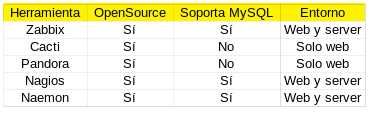
\includegraphics[scale=0.4]{imagenes/comparativanaemon.png}
	\caption{Comparativa a nivel de sistema } \label{comparativa1}
\end{figure}
Como se puede observar, Nagios y Naemon cuentan con mejores características a nivel sistema operativo, ya que se pueden configurar los entornos y los protocolos, que a diferencia de otras aplicaciones no disponen, por lo que se hace más manejable y útil la utilización de Nagios y Naemon.

\subsection{A nivel aplicación} 

\begin{figure}[H]
	\centering
	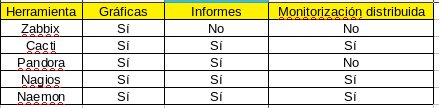
\includegraphics[scale=0.4]{imagenes/comparativanaemon2.png}
	\caption{Comparativa a nivel de aplicación } \label{comparativa2}
	
\end{figure}
\newpage
La visualización mediante gráficas, permite el poder visualizar en tiempo real todas las alertas que van apareciendo, exposición de la información de los chequeos mediante gráficas, para poder visualizar en tiempo real las alertas que van a apareciendo en el sistema. 
\subsection{A nivel extensiones} 
\begin{figure}[H]
	\centering
	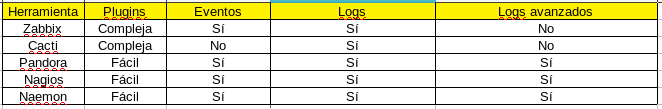
\includegraphics[scale=0.4]{imagenes/comparativanaemon3.png}
	\caption{Comparativa a nivel de extensiones } \label{comparativa3}
	
\end{figure}
Como conclusión de las posibles herramientas que dan solución a algunos de
los problemas que se están valorando, hay que destacar que existen varias que
dan solución a algunos de los problemas, pero no al mismo nivel al que se
pretende llegar, que con Nagios o Naemon se puede fácilmente. 

A la hora de realizar la selección de la herramienta entre las que hemos comentado anteriormente, cabe destacar que todas cumplen con las necesidades que pueda surgir en cualquier red a monitorizar. Por lo que para seleccionar una, se ha decidido tomar como referencia que \textbf{Naemon} se trata de un fork de Nagios, por lo que contará con todas las funcionalidades de éste, además  de contar con  un mejor rendimiento, un funcionamiento más estable y, sobre todo, una nueva interfaz gráfica mucho más ligera, moderna y rápida.  Esta nueva interfaz de Naemon, llamada, \textbf{Thruk Monitoring Webinterface}, es mucho más rápida, moderna y práctica respecto a la que aporta la suite Nagios.

\section{Introducción de Naemon}
\subsection{Funcionamiento Naemon} 
Como se ha mencionado anteriormente Naemon está basado en Nagios exactamente en la \textbf{versión 4.0.2}, el cual cumple su misma función el poder representar la monitorización del sistema, a través de los host y servicios que queramos especificar, teniendo información sobre los cambios mediante las alertas que ofrece este sistema, además de informar cuando la situación empeora o mejora.\cite{naemon}

\textbf{Naemon} se compone de dos partes, \textbf{Naemon Core y la interfaz de monitorización de Thruk}, hablaremos de ella más adelante en este capítulo, aunque es posible aplicar otra interfaz de monitorización, en todo el despliegue del proyecto se aplicará el uso de esta interfaz.

Entre las características que incluye Naemon podemos encontrar:
\begin{itemize}
	\item Monitorización de servicios de red como SMTP, POP3, HTTP, NNTP, PING, entre otros.
	\item Monitorización de los recursos del host como puede ser la carga del procesador, el uso del disco, etc.
	\item Diseño de archivos plugins que permiten a los usuarios desarrollar fácilmente sus propios controles de servicio.
	\item Controles de servicios paralelos.
	\item Thruk Monitoring Webinterface para editar la configuración y ver el estado actual de la red, el historial de problemas, los archivos de registro, los informes de sla, los paneles de control, los procesos empresariales, etc.
	\item Capacidad para definir la jerarquía de hosts de la red mediante hosts "principales", lo que permite la detección y distinción entre los hosts que están inactivos y los que no están disponibles.
	\item Avisos de contacto cuando se producen problemas con el servicio o el host y se resuelven.
	\item Capacidad para definir controladores de eventos que se ejecutarán durante el servicio o eventos de host para la resolución proactiva de problemas.
	\item Rotación automática de archivos de registro.
	\item Soporte para implementar hosts de monitoreo redundantes.
\end{itemize}

Para la monitorización de hosts y servicios, Naemon al igual que Nagios utiliza \textbf{plugins}. Se tratan de componentes externos a los que Naemon les pasa información sobre el cometido que debe realizar, es decir, lo que debe comprobarse y los límites críticos y de advertencia. Una vez sea transmitida dicha información, los plugins harán las respectivas comprobaciones y analizarán los resultados.
\newpage
Dicho resultado del chequeo podrá tener cuatro resultados: \textbf{OK, WARNING, CRITICAL y UNKNOWN}, además de información detallada de los mismos. Así de esta manera Naemon además de encontrar o notificar problemas, previene a cualquier organización que lo implemente, para no tenerlos en un futuro.

Toda esta información se recoge en un único servidor Naemon y así se puede acceder a toda la información de la infraestructura desde una única máquina.
\subsubsection{Archivo de configuración principal}
El archivo de configuración principal contiene una serie de directivas que afectan el funcionamiento del daemon de \textbf{Naemon-core}. Este archivo de configuración es leído tanto por el demonio \textbf{Naemon} como por \textbf{Thruk}, anteriormente conocido como \textbf{$"CGIs"$}. Thruk proporciona una forma sencilla de editar la configuración de Naemon en la interfaz web sin tener que usar el terminal.

El \textbf{archivo de configuración principal} es normalmente llamado \textbf{naemon.cfg} y se encuentra en la carpeta \textbf{/etc/naemon/} \cite{naemoncfg}.

\begin{figure}[H]
	\centering
	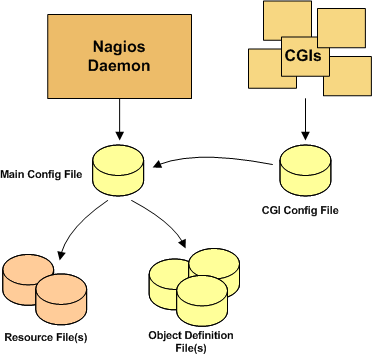
\includegraphics[width=0.7\textwidth]{imagenes/main_configuring/main_configuring.png}
	\caption{Configuración de Naemon\cite{config}}\label{configuration}
\end{figure}

La forma en la que se encuentran los \textbf{archivos de configuración de Naemon} es similar a como se encuentran en \textbf{Nagios}, al ser este un fork de él. Todo esto viene representado en la \textbf{figura \ref{configuration}.}

\subsubsection{Objetos}
La configuración de los distintos equipos y servicios a monitorizar se puede realizar a través de la carpeta \textbf{/etc/naemon/conf.d}, aquí podremos añadir equipos o hosts a la red, además podemos realizar una mejor gestión de la red.

Una de las características del formato de configuración de objetos de Naemon es que puede crear definiciones de objetos que heredan de otros.

A continuación, se explican los distintos objetos más interesantes que podemos añadir en esta \textbf{carpeta}:

\paragraph{Hosts}

Desde la carpeta \textbf{/etc/naemon/conf.d} se pueden añadir equipos a la configuración. Para ello, solo hay que crear una fichero \textbf{hosts.cfg} y además se debe conocer la dirección IP del dispositivo, el tipo de dispositivo (equipo Linux, Windows server, impresora, router o switch), sus ajustes preestablecidos, establecer los periodos de chequeo y de notificación.

A parte de esto se pueden definir relaciones entre hosts mediante el objeto \textit{\textbf{parent hosts}} que permite definir la topología de la infraestructura. Los equipos padres suelen ser routers, switches, firewalls, etc. que se encuentran entre el equipo de monitorización y
un host remoto y que se encargan de transmitir tráfico de paquetes entre ambos. Si el estado de una máquina es inaccesible puede deberse a que su \textbf{parent host},es decir, su padre original, se haya caído. \cite{naemoncfg}

Además, se pueden crear grupos que engloben a varios dispositivos que por ejemplo vayan a utilizar los mismos servicios o tengan características similares para facilitar así su monitorización y organización. El host se guardará en una base de datos.
\newpage
Uno de los principales beneficios es que esta carpeta permite a los usuarios definir plantillas y ajustes preestablecidos que pueden aplicarse al agregar hosts. Un host preestablecido contiene todos los servicios que se deben agregar a un host con todos los comandos vinculados y todos los valores predeterminados establecidos. También contiene el comando \textit{\textbf{check-host-alive}} que se aplicará al nuevo host. Al añadir un host, el usuario debe ajustar algunos parámetros para adecuar la monitorización del host a su caso específico.

Naemon viene por defecto con unas plantillas predefinidas que hacen referencia a varios posibles tipos de máquinas. En cualquier caso, y como bien se ha dicho antes, el usuario puede añadir más sistemas desde \textbf{/etc/naemon/conf.d} en la parte de additional items y advanced
items. Su formato de definición es el correspondiente a la \textbf{figura \ref{define-hosts}.}
\begin{figure}[H]
	\centering
	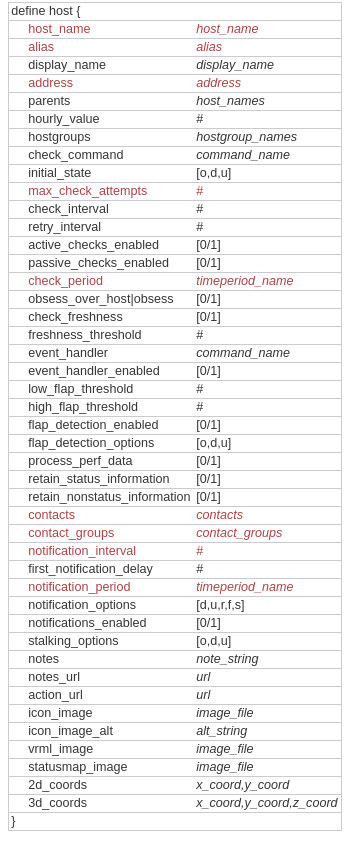
\includegraphics[scale=0.4]{imagenes/definicion_objetos/hosts.png}
	\caption{Formato de definición de un objeto de tipo Host} \label{define-hosts}	
\end{figure}
A continuación se va explicar las distintas directivas que se pueden encontrar a la hora de definir un host:
\begin{itemize}
	\item \textbf{host\_name}: se usa para definir el identificador del host con un nombre corto.
	\item \textbf{alias}: se usa para definir un nombre o una descripción para identificar el host.	
	\item \textbf{display\_name}: se utiliza para definir un nombre alternativo que debe mostrarse en la interfaz web para este host.
	\item \textbf{address}: se utiliza para definir la dirección del host. Normalmente, esta es una dirección IP, aunque realmente podría ser cualquier cosa que desee. 
	\item \textbf{parents}: se utiliza para definir una lista delimitada por comas de nombres cortos de los \textbf{hosts principales} para este host en particular.
	\item \textbf{hostgroups}: se utiliza para identificar los nombres cortos de los grupos de hosts a los que pertenece el host.
	\item \textbf{check\_command}: se usa para especificar el nombre corto del comando que se debe usar para verificar si el host está activo o inactivo.
	\item \textbf{initial\_state	[o,d,u]}: por defecto, Naemon asumirá que todos los hosts están en estado UP cuando se inicia. Puede anular el estado inicial de un host utilizando esta directiva. \textit{Las opciones válidas son: o = ARRIBA, d = ABAJO, y u = INACTIVO.}
	\item \textbf{max\_check\_attempts}: se utiliza para definir la cantidad de veces que Naemon volverá a intentar el comando de verificación de host si devuelve cualquier estado que no sea OK. Establecer este valor en 1 hará que Naemon genere una alerta sin volver a intentar la verificación del host.	
	\item \textbf{check\_interval}: se utiliza para definir el número de `unidades de tiempo'  entre las comprobaciones programadas regularmente del host.	
	\item \textbf{retry\_interval}: se utiliza para definir el número de `unidades de tiempo' que debe esperar antes de programar una nueva verificación de los hosts. 	
	\item \textbf{active\_checks\_enabled}: se utiliza para determinar si las comprobaciones activas de este host están habilitadas. 
	\item \textbf{passive\_checks\_enabled}: se utiliza para determinar si las comprobaciones pasivas están habilitadas o no para este host. 	
	\item \textbf{check\_period}: se utiliza para especificar el nombre corto del período de tiempo durante el cual se pueden realizar verificaciones activas de este host.	
	\item \textbf{process\_perf\_data}: se utiliza para determinar si el procesamiento de datos de rendimiento está habilitado o no para este host.	
	\item \textbf{event\_handler\_enabled}:	se utiliza para determinar si el controlador de eventos para este host está habilitado o no. 
	\item \textbf{retain\_status\_information}: se utiliza para determinar si la información relacionada con el estado del host se retiene o no en los reinicios del programa.	
	\item \textbf{retain\_nonstatus\_information}: se utiliza para determinar si la información que no es de estado sobre el host se retiene en los reinicios del programa. Esto solo es útil si ha habilitado la retención de estado utilizando la direc	
	\item \textbf{contacts}: Esta es una lista de los nombres cortos de los contactos que se deben notificar siempre que haya problemas con este host.	
	\item \textbf{contact\_groups}: Esta es una lista de los nombres cortos de los grupos de contacto que se deben notificar siempre que haya problemas con este host.	
	\item \textbf{notification\_interval}: se utiliza para definir el número de "unidades de tiempo" que esperar antes de volver a notificar a un contacto que este servicio aún está inactivo o inaccesible.	
	\item \textbf{notification\_period}: se utiliza para especificar el nombre corto del período de tiempo durante el cual se pueden enviar notificaciones de eventos para este host a los contactos.	
	\item \textbf{notification\_options	[d,u,r,f,s]}: se utiliza para determinar cuándo se deben enviar notificaciones para el host. Las opciones válidas son una combinación de uno o más de los siguientes: d = enviar notificaciones en estado ABAJO, u = enviar notificaciones en estado NO ALCANZABLE, r = enviar notificaciones en recuperaciones (estado correcto), f = enviar notificaciones cuando se inicia el host y deja de aletear, y s = envía notificaciones cuando comienza y termina el tiempo de inactividad programado. 
	\item \textbf{notifications\_enabled}: se utiliza para determinar si las notificaciones para este host están habilitadas o no.	
\end{itemize}

\paragraph{Servicios}

El poder de esta herramienta de monitorización reside en los servicios que se pueden monitorizar. Estos pueden ser tanto servicios públicos como privados.  \cite{naemoncfg}

Un \textbf{servicio} es “\textit{público}” cuando es accesible a través de la red, ya sea en la red local o por Internet como \textbf{HTTP, POP3, IMAP, FTP y SSH}. Estos servicios y aplicaciones, así como sus protocolos, pueden ser monitorizados por Naemon sin necesidad de requerimientos de acceso especiales.

En cambio, los servicios “\textit{privados}” no pueden ser monitorizados con Naemon sin la intervención de algún agente. Ejemplos de servicios privados asociados con los equipos son la carga de CPU, uso de memoria, uso en disco, cuentas de usuarios activos, información de procesos, etc. Estos servicios privados o atributos de los equipos usualmente no son expuestos a clientes externos. Esta situación requiere que un agente intermediario sea instalado en el equipo que se desea monitorizar esa información.

Sobre los dispositivos que hemos configurado anteriormente podemos añadir diferentes servicios de monitorización. Para ver la disponibilidad de dichas máquinas es conveniente añadir a todos ellos el servicio \textbf{PING} \cite{monitoring} que \textit{nos hará saber si ese ordenador está configurado en la red y nos notificará si alguno de ellos cae en un momento dado}, es decir, \textit{permite hacer una verificación del estado de una determinada conexión o host local}. \textbf{PING} se encuentra en la mayoría de sistemas operativos incluyendo Unix y Windows. Cabe mencionar que este servicio se encuentra desactivado en Windows por defecto.

A la hora de definir servicios es obligatorio fijar unos intervalos de chequeo del servicio y de notificación de los mismos por si alguno de ellos da algún problema a la hora de ser monitorizado. Los parámetros que definen estos periodos son los mismos que en los hosts.

En los servicios también se pueden definir plantillas con una serie de servicios a monitorizar definidos para una mayor facilidad, por ejemplo, si se quieren definir dichos servicios en múltiples equipos (en vez de tener que añadir cada servicio uno a uno, se añadirían todos los servicios de una vez).

Como en el caso de las máquinas, los servicios también se pueden agrupar. Estas agrupaciones sirven para manejar de una manera más efectiva los servicios, que sea más organizado a la hora de ver la información de los mismo en las interfaces web y para configurar dependencias entre equipos.
Su formato de definición es el de la figura \ref{define-services}.
\begin{figure}[H]
	\centering
	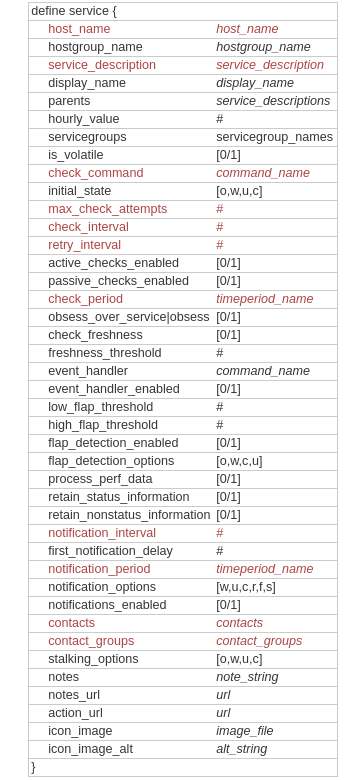
\includegraphics[scale=0.4]{imagenes/definicion_objetos/services.png}
	\caption{Formato de definición de un objeto de tipo Servicios} \label{define-services}
\end{figure}

A continuación se va explicar las distintas \textbf{directivas} que se pueden encontrar a la hora de definir un servicio, algunas son parecidas en cuanto a la funcionalidad como las usadas para definir un host:
\begin{itemize}
	\item 	\textbf{host\_name}: se utiliza para especificar los nombres abreviados de los hosts en los que el servicio se ejecuta o está asociado.	
	\item \textbf{hostgroup\_name}:	se utiliza para especificar los nombres abreviados de los grupos de hosts en los que el servicio se ejecuta" o con los que está asociado. 
	\item \textbf{service\_description}: se utiliza para definir la descripción del servicio, que puede contener espacios, guiones y dos puntos.
	\item \textbf{hourly\_value}:se utiliza para representar el valor del servicio.	
	\item \textbf{servicegroups}: se usa para identificar los nombres abreviados de los grupos de servicios a los que pertenece el servicio. Varios grupos de servicio deben estar separados por comas. 	
	\item \textbf{is\_volatile}: se utiliza para denotar si el servicio es volátil. Los servicios normalmente no son volátiles. 
	\item \textbf{check\_command}: se utiliza para especificar el nombre corto del comando que ejecutará Naemon para verificar el estado del servicio. 	
	\item \textbf{initial\_state [o,w,u,c]}: por defecto, Naemon asumirá que todos los servicios están en estado OK cuando se inicia. Puede anular el estado inicial de un servicio utilizando esta directiva. Las opciones válidas son: o = OK, w = ADVERTENCIA, u = DESCONOCIDO, y c = CRÍTICO.
	\item \textbf{max\_check\_attempts}:se utiliza para definir la cantidad de veces que Naemon volverá a intentar el comando de verificación de servicio si devuelve cualquier estado que no sea OK. 	
	\item \textbf{check\_interval}: se utiliza para definir el número de \textit{unidades de tiempo} a esperar antes de programar la próxima verificación \textit{regular} del servicio	
	\item \textbf{retry\_interval}:se utiliza para definir el número de \textit{unidades de tiempo} a esperar antes de programar una nueva verificación del servicio.	
	\item \textbf{active\_checks\_enabled}: se utiliza para determinar si las comprobaciones activas de este servicio están habilitadas o no. 	
	\item \textbf{passive\_checks\_enabled}: se usa para determinar si las comprobaciones pasivas de este servicio están habilitadas o no	
	\item \textbf{check\_period}: se utiliza para especificar el nombre corto del período de tiempo durante el cual se pueden realizar verificaciones activas de este servicio.	
	\item \textbf{obsess\_over\_service$|$obsess}: determina si las comprobaciones para el servicio estarán \textit{sobrecargadas} con el uso del comando \textit{ocsp\_command}.
	\item \textbf{check\_freshness}: se utiliza para determinar si las comprobaciones de actualización están habilitadas o no para este servicio. 	
	\item \textbf{freshness\_threshold}: se utiliza para especificar el umbral de actualización (en segundos) para este servicio. 	
	\item \textbf{event\_handler}: se utiliza para especificar el nombre corto del comando que debe ejecutarse cada vez que se detecta un cambio en el estado del servicio. 	
	\item \textbf{event\_handler\_enabled}: se utiliza para determinar si el controlador de eventos para este servicio está habilitado o no.
	\item \textbf{low\_flap\_threshold}: se utiliza para especificar el umbral de cambio de estado bajo utilizado en la detección de aletas para este servicio.  	
	\item \textbf{high\_flap\_threshold}: se utiliza para especificar el umbral de cambio de estado alto utilizado en la detección de aletas para este servicio. 	
	\item \textbf{flap\_detection\_enabled}: se utiliza para determinar si la detección de flaps está habilitada o no para este servicio.	
	\item \textbf{flap\_detection\_options	[o,w,c,u]}: se usa para determinar qué estados de servicio utilizará la lógica de detección de aletas para este servicio. Las opciones válidas son una combinación de uno o más de los siguientes: o = estados OK, w = estados de ADVERTENCIA, c = estados CRÍTICOS, u = estados DESCONOCIDOS.
	\item \textbf{process\_perf\_data}:se utiliza para determinar si el procesamiento de datos de rendimiento está habilitado o no para este servicio. 	
	\item \textbf{retain\_status\_information}: se usa para determinar si la información relacionada con el estado del servicio se retiene o no en los reinicios del programa.
	\item \textbf{retain\_nonstatus\_information}: se usa para determinar si la información que no es de estado sobre el servicio se retiene o no en los reinicios del programa.	
	\item \textbf{notification\_interval}: se utiliza para definir el número de \textit{unidades de tiempo} que esperar antes de volver a notificar a un contacto que este servicio todavía está en un estado no correcto. 	
	\item \textbf{first\_notification\_delay}: se usa para definir el número de \textit{unidades de tiempo} que esperar antes de enviar la primera notificación de problema cuando este servicio entra en un estado no correcto. 
	\item \textbf{notification\_period}: se utiliza para especificar el nombre corto del período de tiempo durante el cual se pueden enviar notificaciones de eventos para este servicio a los contactos. 
	\item \textbf{notification\_options	[w,u,c,r,f,s]}: se utiliza para determinar cuándo se deben enviar notificaciones para el servicio. Las opciones válidas son una combinación de uno o más de los siguientes: w = enviar notificaciones en estado de ADVERTENCIA, u = enviar notificaciones en estado DESCONOCIDO, c = enviar notificaciones en estado CRÍTICO, r = enviar notificaciones en recuperaciones (estado correcto), f = envía notificaciones cuando el servicio comienza y deja de aletear, y s = envía notificaciones cuando comienza y termina el tiempo de inactividad programado. 
	\item \textbf{notifications\_enabled}: se usa para determinar si las notificaciones para este servicio están habilitadas o no.	
	\item \textbf{contacts}: es una lista de los nombres cortos de los contactos que deben notificarse siempre que haya problemas con este servicio. Los contactos múltiples deben estar separados por comas.	
	\item \textbf{contact\_groups}: es una lista de los nombres cortos de los grupos de contacto que deben notificarse siempre que haya problemas con este servicio. Múltiples grupos de contacto deben estar separados por comas. 	
\end{itemize}
\paragraph{Comandos}

Los \textbf{comandos} definen cómo se deben hacer los chequeos de hosts y servicios, y cómo deben funcionar las notificaciones. Otra de sus funciones es restablecer el sistema automáticamente si es posible. \cite{naemoncfg}

La propia imagen de Naemon incluye una serie de comandos preestablecidos basados en plugins que son los que chequean los distintos servicios (SSH, HTTP, etc.) pero también el usuario puede añadir sus propios comandos.

Las definiciones  de los comandos pueden contener macros, pero se debe asegurar de incluir solo aquellas que son "validas" para las circunstancias en que se usará el comando.

A la hora de realizar la definición de un objeto de tipo \textbf{Comando} Naemon especifica una forma concreta a la hora de establecer sus directivas concretas, dicha forma viene representada en la figura \ref{define-command} donde se puede apreciar el uso de la directiva \textbf{command\_name} que se encarga de asignar un nombre al comando y \textbf{command\_line} encargada de especificar el formato de línea del comando, es decir, cómo se verá en la \textbf{shell de Naemon}. 

\begin{figure}[H]
	\centering
	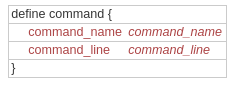
\includegraphics[scale=0.5]{imagenes/definicion_objetos/command.png}
	\caption{Formato de definición de un objeto de tipo Comandos} \label{define-command}	
\end{figure}
\newpage
\paragraph{Contactos}

Los contactos hacen referencia a diferentes personas que pueden ser los propietarios de diferentes máquinas, encargados de gestionar y solucionar problemas que pueden surgir en los dispositivos, destinatarios de notificaciones, etc.

A la hora de crear un contacto solo es obligatorio un nombre, un alias y una dirección de email. También se pueden definir los periodos de notificación de equipos y servicios y que tipo de notificaciones han de ser enviadas al contacto.

Los contactos se asignan a los usuarios que inician sesión en una de las interfaces web y todas las operaciones que se realicen a través de esa interfaz quedarán registradas como ese usuario y se permitirán dependiendo del acceso que tenga dicho usuario a determinados servicios. 

Los contactos también pueden ser agrupados en \textbf{contact groups} para dividir tareas y responsabilidades entre, por ejemplo, los empleados de una empresa. Así, por ejemplo, las notificaciones de los servicios irán destinadas a un grupo de trabajo y las de los dispositivos a otro.

Su formato de definición es el de la figura \ref{define-contact}. 
\begin{figure}[H]
	\centering
	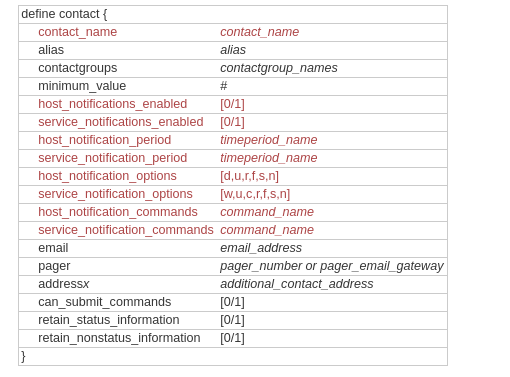
\includegraphics[scale=0.7]{imagenes/definicion_objetos/contact.png}
	\caption{Formato de definición de un objeto de tipo Contacto} \label{define-contact}
	
\end{figure}

\paragraph{Time Periods}

Los \textbf{time periods} son definiciones de periodos de tiempo en los que se pueden realizar los chequeos o se pueden enviar notificaciones de equipos y servicios. Estas definiciones se aplican a la hora de definir equipos y servicios en los parámentros check period y notification period.

Naemon trae predefinidos algún time period pero el usuario puede añadir los suyos propios. Solo hace falta un nombre único, un alias y el tiempo que se quiera definir.

Su formato de definición es el de la figura \ref{time-period}. 


\begin{figure}[H]
	\centering
	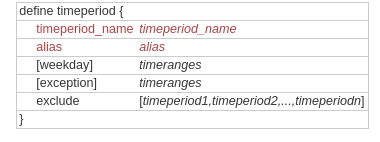
\includegraphics[scale=0.7]{imagenes/definicion_objetos/time_period.png}
	\caption{Formato de definición de un objeto de tipo Time-Period} \label{time-period}	
\end{figure}

\paragraph{Plantillas}

Como ya se ha mencionado anteriormente, Naemon permite crear \textbf{plantillas} para definir parámetros comunes que puedan ser aplicados a la hora de definir nuevos equipos y servicios.

Cuando se aplica una plantilla a un host o servicio, éste adquiere todas las propiedades definidas en la plantilla. Es posible aplicar varias plantillas a un único equipo. Si las plantillas especifican un mismo parámetro, predominará el valor del parámetro de la primera plantilla.

\subsubsection{Thruk}

\textbf{Thruk}\cite{thruk} se trata de una interfaz de monitorización \textbf{multibackend}, es decir, puede emplear una gran variedad de backends, es decir, exactamente servidores backend como es el caso de Naemon, además de herramientas como Nagios y otras muchas más, todas ellas utilizando como API la llamada \textbf{LiveStatus API} \cite{livestatus}. Está diseñado para ser un reemplazo de la herramienta y básicamente cubrir las tareas de la herramienta al completo, añadiendo grandes instalaciones y haciendo así que incrementa su usabilidad.

\textbf{Thruk} viene organizado con la siguiente estructura reflejada en la figura \ref{thruk}. Teniéndose que su autenticación HTTP viene bajo el servidor web de Apache y corriendo bajo un servidor \textbf{Fast CGI} se conecta a Naemon a través de una conexión por el puerto correspondiente a TCP/IP.

\begin{figure}[H]
	\centering
	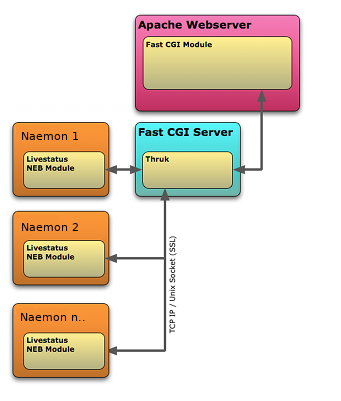
\includegraphics[scale=0.7]{imagenes/thruk/arquitectura.png}
	\caption{Estructura de conexión de Thruk} \label{thruk}
\end{figure}

A través de la página \url{https://www.thruk.org/demo.html} se puede realizar pruebas de la demo de dicha interfaz.

Entre las principales \textbf{ventajas}  de Thruk encontramos:
\begin{itemize}
	\item Múltiples backends, esto es que podemos aplicar como servidor, se pueden incluir los siguientes:\textbf{Naemon, Nagios, Icinga y Shinken}.
	Supongamos que tiene una antigua instalación de Nagios heredada aún en producción, además de un nuevo servidor Naemon o Icinga 2. Con Thruk puede configurar ambos como backends para Thruk, y le dará una vista unificada para todos los hosts y servicios configurados. Una pestaña menos en su navegador.
	\newpage
	\item Thruk tiene muchas características excelentes, pero lo primero que notas es la velocidad. Incluso una configuración con miles de hosts y decenas de miles de servicios tiene tiempos de respuesta inferiores al segundo para los listados de servicios y los resultados de búsqueda.
	\item Thruk también tiene la opción de modificar su interfaz web clásica que lo hace un poco más fácil de usar y expande la funcionalidad de monitorización e informes.
	\item Muestra en vivo la información.
	\item Fácil incorporación de plugins, tanto plugins propios de Thruk, como plugins adicionales de Naemon en este caso.	
\end{itemize}
\textbf{Thruk} viene de forma nativa con Naemon, y es una interfaz web de reemplazo completa y gratuita de código abierto para Nagios, Icinga y Shinken. Estas son herramientas flexibles para alertarnos cuando algo sale mal, y Thruk se encarga de garantizar una correcta monitorización.

Al ser una interfaz nativa de \textbf{Naemon} es preferible su utilización, puesto que su forma de integración y modificación de sus diferentes elementos será mucho menos complejo que con otras interfaces.

\subsubsection{Plugins}
A diferencia de muchas otras herramientas de monitorización, Naemon no incluye ningún mecanismo interno para verificar el estado de los hosts y servicios en su red. En su lugar, Naemon se basa en programas externos llamados \textbf{plugin} para hacer todo el trabajo.

Entonces los plugins son ejecutables o scripts (normalmente en perl, python, shell, entre otros) que se pueden ejecutar desde una línea de comandos para verificar el estado de un host o de un servicio concreto del host. Naemon usa los resultados de los plugins para determinar el estado actual de los hosts y servicios en su red. \cite{NaemonPlugins}

\textbf{Naemon} ejecutará un plugin siempre que sea necesario verificar el estado de un host o un servicio concreto del host. El plugin hace algo para realizar la comprobación y luego simplemente devuelve los resultados a Naemon. Naemon procesará los resultados que recibe del plugin y tomará las medidas necesarias.
\newpage
Los \textbf{plugins} \ref{plugin} actúan como una capa de abstracción entre la lógica de supervisión presente en el demonio de Naemon y los servicios y hosts reales que se están supervisando.

La ventaja de este tipo de arquitectura de plugins es que puede monitorear cualquier elemento.

\begin{figure}[H]
	\centering
	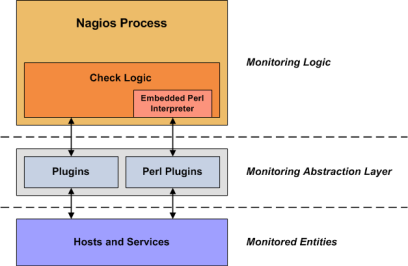
\includegraphics[scale=0.7]{imagenes/main_configuring/plugins.png}
	\caption{Funcionamiento de los plugins en Naemon} \label{plugin}	
\end{figure}

La \textbf{desventaja} de este tipo de arquitectura de plugin es el hecho de que Naemon no tiene reflejo de qué es lo que está monitorizando, simplemente rastrea los cambios en el estado de esos recursos.

Solo los plugin saben exactamente lo que están monitorizando y cómo realizar las comprobaciones reales.

Los \textbf{plugins de Naemon} no se distribuyen, pero se pueden descargar plugins de Naemon y plugins adicionales desde las siguientes \textbf{páginas}:
\begin{itemize}
	\item \textbf{Proyecto de Monitorización de Complementos: } \url{http://monitoring-plugins.org} 
	\item \textbf{Proyecto de complementos de Nagios: } \url{https://nagios-plugins.org/} 
	\item\textbf{ Nagios Exchange: } \url{http://exchange.nagios.org/}
\end{itemize}
\newpage
Hemos mencionado que Naemon se trata de un fork de Nagios, por lo que la compatibilidad y uso de sus plugins será totalmente aceptable, por lo que podemos usar cualquier plugins de la base de datos de Nagios en Naemon.
\chapter{Despliegue de Naemon} \label{ch:despliegue}
En este capítulo profundizaremos en la realización del \textbf{despliegue de Naemon}, introduciendo el entorno que se ha utilizado para su despliegue, comparando herramientas y seleccionando la que mejor se adecua a nuestras necesidades. Además se expondrá la configuración correspondiente para poder realizar ese despliegue desde la instalación rudimentaria hasta su prueba básica aplicando un plugin correspondiente.

\section{Entorno del despliegue}
A la hora de hablar de un \textbf{entorno de despliegue} nos referiremos a una instancia específica de una configuración de hardware y software establecida con el fin de instalar y ejecutar el software desarrollado para este uso.

Por lo que básicamente un entorno de despliegue lo trataremos como una colección de clústeres y servidores configurados que colaboran para proporcionar un entorno que aloje módulos de software concretos.

\subsection{Alternativas a utilizar}
A continuación se expondrán los posibles entornos a aplicar y se concluirá con la opción seleccionada.
\newpage
\subsubsection{Entorno nativo}
Un \textbf{entorno nativo} lo definiremos como el entorno que se encuentra instalado directamente sobre un sistema anfitrión ejecutándose en hardware físico.

Al trabajar sobre el propio hardware contará con la ventaja de dedicar sus propios recursos a la hora de garantizar el mejor rendimiento.

Pero tiene la desventaja de que si existe algún problema de seguridad o alguna intrusión se efectuará sobre el propio sistema anfitrión. Otra desventaja es que es difícil controlar un backup en el caso de perder o no realizar ese backup.

Esta opción la descartaremos ya que es poco aconsejable utilizar entornos de desarrollo en nuestra máquina de forma local, ya que supone tener instaladas versiones del software que el desarrollador necesite en cada momento. Además sería una opción bastante compleja de controlar, teniéndose así una carga de trabajo adicional para el usuario, debido al tiempo que debe invertir en solucionar los problemas que puedan surgir debido a que algún empleado haya cambiado algo en su máquina local.

Por lo que será preferible que a la hora de desarrollar se trabaje bajo virtualización, evitando así los problemas que puedan surgir en una máquina local, ya que permite la creación de máquinas virtuales iguales para cada miembro de por ejemplo un equipo de desarrollo.
\subsubsection{Entorno virtual o máquina virtual}
El concepto de este término es que se trata de un sistema operativo completo funcionando de manera aislada sobre otro sistema operativo completo.

Este tipo de entorno permite compartir el hardware de forma que lo puedan utilizar varios sistemas operativos al mismo tiempo.
\newpage
Un esquema de esta arquitectura es el mostrado en la figura \ref{virtual}.
\begin{figure}[H]
	\centering
	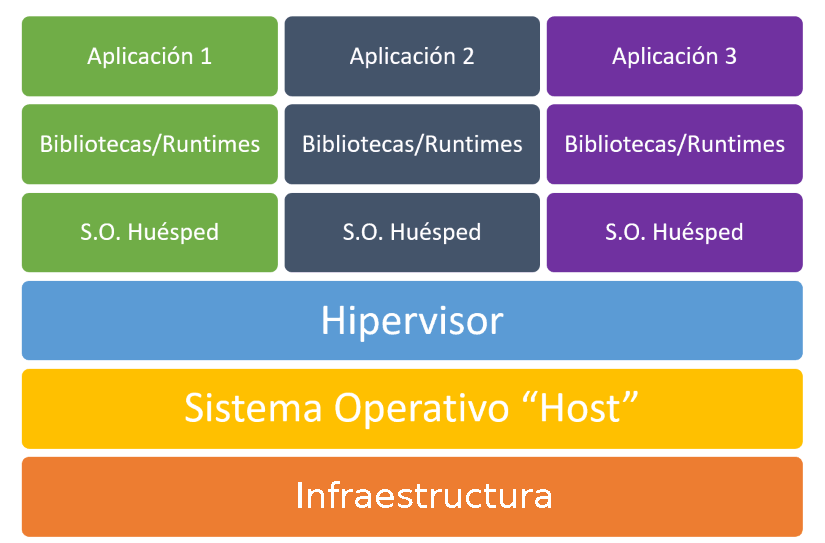
\includegraphics[width=0.4\textwidth]{imagenes/entorno/virtual.png}
	\caption{Arquitectura de un entorno virtual} \label{virtual}
\end{figure}
Por debajo del sistema operativo siempre estará la infraestructura, por ejemplo el ordenador personal para realizar cualquier desarrollo, o si es por ejemplo un despliegue real se usará un servidor.

Para que una \textbf{máquina virtual} pueda ejecutarse es necesario la instalación del \textbf{hipervisor} que se trata de un software especializado en exponer los recursos hardware que están debajo del sistema operativo, de forma que puedan ser utilizados por otros sistemas operativos. Los hipervisores vienen como productos como Hyper-V, VirtualBox o VMWare, entre otros.

Gracias a todo esto podemos tener diferentes sistemas operativos ejecutándose en paralelo sobre la misma máquina física, cada uno con su memoria y espacio en disco reservados, y completamente aislados unos de otros.
\subsubsection{Aplicación de contenedores}

La filosofía de los contenedores es totalmente diferente a la de las máquinas virtuales. Si bien tratan también de aislar a las aplicaciones y de generar un entorno replicable y estable para que funcionen, en lugar de albergar un sistema operativo completo lo que hacen es compartir los recursos del propio sistema operativo "host" sobre el que se ejecutan.
\newpage
Su esquema viene estructurado de la forma en la que viene representado en la figura \ref{contenedores}.

\begin{figure}[H]
	\centering
	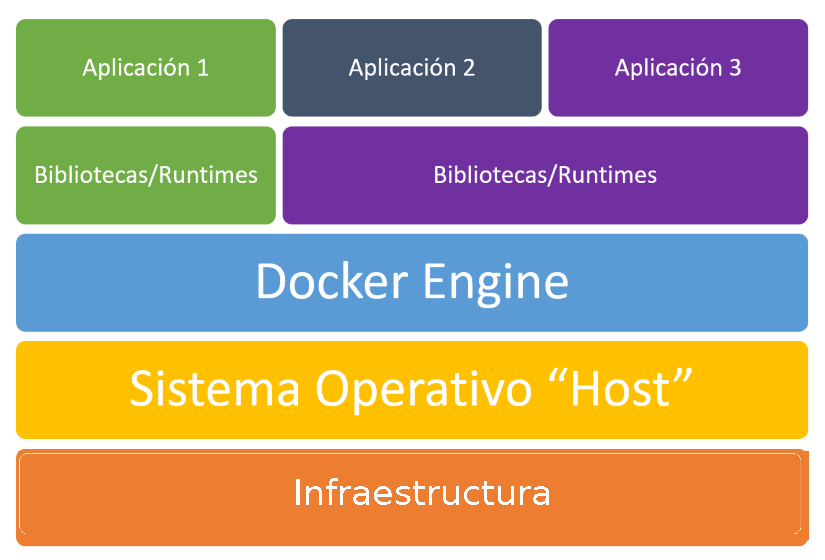
\includegraphics[width=0.4\textwidth]{imagenes/entorno/contenedores.png}
	\caption{Estructura de un entorno con contenedores} \label{contenedores}
\end{figure}
En primer lugar debemos tener en cuenta que, en el caso de los contenedores, el hecho de que no necesiten un sistema operativo completo sino que reutilicen el subyacente reduce mucho la carga que debe soportar la máquina física, el espacio de almacenamiento utilizado y el tiempo necesario para lanzar las aplicaciones. Por lo tanto los contenedores son mucho más ligeros que las máquinas virtuales.

Cuando definimos una máquina virtual debemos indicar de antemano cuántos recursos físicos le debemos dedicar. En el caso de los contenedores esto no es así. De hecho no indicamos qué recursos vamos a necesitar, sino que en función de las necesidades de cada momento, el encargado de asignar lo que sea necesario para que los contenedores funcionen adecuadamente.

Esto hace que los entornos de ejecución en contenedores sean mucho más ligeros, y que se aproveche mucho mejor el hardware, además de permitir levantar muchos más contenedores que máquinas virtuales en la misma máquina física. Mientras que una máquina virtual puede tardar un minuto o más en arrancar y tener disponible nuestra aplicación, un contenedor se levanta y responde en unos pocos segundos. El espacio ocupado en disco es muy inferior con los contenedores al no necesitar que instalemos el sistema operativo completo.

Además para realizar despliegues avanzados de aplicaciones en contenedores hay que ir más allá y utilizar tecnologías que nos permiten orquestar y controlar los despliegues con muchas partes en ejecución.

Como desventajas se tiene que no pueden sustituir por completo la virtualización tradicional y no todo el mundo cuenta de un modelo de negocio que sea compatible a estos.

También aumentan riesgos de brechas de seguridad, además cuentan con menos flexibilidad a nivel de sistema operativo del contenedor.

Dejar de usar sistemas operativos separados implica una mejora en el rendimiento de la virtualización con contenedores, pero significa también tener un nivel más bajo de seguridad. En una virtualización del sistema operativo tienen efecto sobre todos los contenedores. 

Todas las soluciones de \textbf{virtualización de contenedores Linux} actuales basan su funcionamiento en una serie de librerias o funcionalidades básicas del kernel y vertebran la arquitectura que da soporte a su funcionamiento. Estos componentes son:

\begin{itemize}
	\item  \textbf{CGROUPs}: se trata de una característica del kernel que permite limitar los recursos del sistema, es decir, limita, contabiliza y aisla el uso de los recursos como puede ser la CPU, la memoria, el disco, etc, para un conjunto de procesos.
	\item \textbf{NAMESPACES}: es un espacio donde uno o mas identificadores de proceso pueden co-existir. Esto permite que tengamos varios PID’s agrupados, pero separados de otros sin que puedan ver qué recursos están utilizando cada uno de los espacios de nombres adyacentes. Existen 6 tipos básicos de \textbf{namespaces} relacionados con
	distintos aspectos del sistema:
	\begin{itemize}
		\item \textbf{NETWORK namespace}: Aislamiento de red. Así, cada namespace de red tendrá sus propias interfaces, direcciones y puertos de red, tablas de enrutamiento,
		etc.
		\item \textbf{PID namespace}: Aísla el espacio de identificadores de proceso. Un contenedor
		tendrá su propia jerarquía de procesos y su proceso padre o init (PID 1).
		\item \textbf{UTS namespace}: Aísla el dominio y hostname, permitiendo a un contenedor
		poseer su propio dominio de nombres.
		\item \textbf{MOUNT namespace}: Aísla los puntos de montaje de los sistemas de ficheros
		que puede ver un grupo de procesos. Este namespace fue el punto de partida,con chroot.
		\item \textbf{USER namespace}: Aísla identificadores de usuarios y grupos. Así dentro un
		contenedor es posible tener un usuario con ID 0 (root) que se corresponda con
		un ID de usuario cualquiera en el host.
		\item \textbf{IPC namespace}: Aísla la intercomunicación entre procesos dentro del espacio
	\end{itemize}
\end{itemize}

En este trabajo usaremos los contenedores por las ventajas mencionadas. A continuación explicaremos algunas herramientas que permiten automatizar aplicaciones a través de contenedores: 
\paragraph{Docker Engine}
\textbf{Docker} \cite{docker} \cite{dockerCE} se trata de un proyecto de software libre que permite automatizar el despliegue de aplicaciones dentro de contenedores. Permitiendo empaquetar una aplicación en una unidad estandarizada para el desarrollo de software, que contiene todo lo necesario para su funcionamiento.
\begin{figure}[H]
	\centering
	
\includegraphics[width=0.4\textwidth]{imagenes/entorno/docker.png}
	\caption{Docker} \label{docker}
\end{figure}

Usa recursos del sistema de forma totalmente aislada, permitiendo asignar recursos o combinaciones de estos recursos entre los procesos que se ejecutan en un sistema.

Los contenedores de imagen de \textbf{Docker} se pueden ejecutar de forma nativa en Linux y Windows. Sin embargo, las imágenes de Windows solo pueden ejecutarse en hosts de Windows y las imágenes de Linux pueden ejecutarse en hosts de Linux y hosts de Windows, donde host significa un servidor o una máquina virtual.

Permite centrarse en el código sin preocuparse de si funcionará en la máquina en la que se ejecutará. Esto acelera el proceso de mantenimiento y desarrollo de cada proyecto y, de cara a DevOps, permite que tanto los desarrolladores como los administradores de sistema pueden probar aplicaciones en un entorno seguro y exactamente igual en todos los casos.

A nivel de arquitectura y componentes, \textbf{Docker} funciona de forma que para proporcionar las características básicas de aislamiento y virtualización emplea las tecnologías que proporciona el Kernel de Linux.

Es un sistema que permite una enorme \textbf{portabilidad} ya que, debido al enorme auge que ha experimentado, la mayor parte de las grandes empresas comerciales de tecnologías de infraestructuras orientadas al cloud computing permiten ejecutar contenedores Docker de forma nativa desde sus plataformas cloud. Destacamos el caso de \textbf{Google Cloud, Amazon AWS y Microsoft Azure} que tienen plataformas nativas especializadas en la ejecución de contenedores Docker con múltiples funcionalidades y tipos de escalabilidad y alta disponibilidad.

Auspiciado por el éxito de las soluciones \textbf{Docker}, podemos encontrar en el mercado un gran numero de aplicaciones comerciales en formato contenedor Docker para ser usadas y arrancadas sin necesidad de conocimientos previos. Del mismo modo, podemos encontrar todo tipo de servicios que se distribuyen preparados para ser usados en formato contenedor Docker, lo que nos permite acceder a desplegar una enorme cantidad de aplicaciones y servicios sin
prácticamente necesidad de un conocimiento previo de los pasos de su instalación, y lo que es más importante, con el soporte directo del fabricante de la solución.

Podemos ver a \textbf{Docker} además de como una herramienta para la creación de contenedores virtuales, como una capa más de abstracción y aislamiento que además aporta un sistema que facilita enormemente la gestión y administración de los contenedores.
\paragraph{OpenShift}
Software creado por \textbf{Red Hat}, fabricante detrás de una de las distribuciones Linux comerciales más extendidas, OpenShift es una solución que permite desplegar aplicaciones realizadas con cualquier stack de tecnologías.\cite{openshift}
\begin{figure}[H]
	\centering
	
\includegraphics[width=0.4\textwidth]{imagenes/entorno/openshift.png}
	\caption{OpenShift} \label{openshift}
\end{figure}
Básicamente, permite al desarrollador centrarse en su trabajo de creación de la aplicación y evitar preocuparse con el mantenimiento de los servicios o la escalabilidad de las aplicaciones. Es capaz de trabajar con lenguajes y frameworks diversos y permite modificar y desplegar las aplicaciones rápidamente bajo demanda, automatizando el proceso entero.

Cuenta con una interfaz bastante intuitiva y manejable. \textbf{Openshift} se basa en Docker y Kubernetes, pero añade una nueva capa.

Es ahora mismo una de las opciones más interesantes para \textbf{Cloud privadas}, ya que está basada en estándares abiertos, integra con las tecnologías open source de referencia y tiene un market en constante crecimiento. 

Aunque está basada en código abierto, y cuenta con versiones gratuitas, no deja de ser un producto de \textbf{RedHat}. Por lo que contará con versiones de pago. 

Como desventaja es que no deja instalar ciertas imágenes o utilizar el usuario root. Cuenta con gestión de imágenes de contenedores con \textbf{ImageStreams} Además tiene integración de la herramienta \textbf{Jenkins}.

\paragraph{CoreOS rkt (rocket)}
Es un  motor de software de automatización de contenedores para ejecutar cargas de trabajo de aplicaciones de forma aislada de la infraestructura subyacente.\cite{rkt}

\begin{figure}[H]
	\centering
	
\includegraphics[width=0.4\textwidth]{imagenes/entorno/rocket.png}
	\caption{CoreOS} \label{rocket}
\end{figure}

Los contenedores CoreOS rkt operan en la mayoría de las principales distribuciones del sistema operativo Linux como un archivo binario que se integra con los sistemas y scripts de inicio de Linux, y opera de acuerdo con el modelo de proceso estándar de Unix, que es una relación padre-hijo. 

Respecto a CoreOS Rkt, este sistema es similar a Docker ya que se encarga de la virtualización de aplicaciones en el propio sistema operativo principal.
\newpage
Algunas de las principales características de este software es que también se ha diseñado pensando en la seguridad por defecto, incluye soporte para \textbf{SELinux} así como para ejecutar aplicaciones en máquinas virtuales aisladas. Otras características es que soporta varios sistemas de inicio como systemd y upstart, por último, también puede ejecutar imágenes Docker.

Como inconvenientes es que existen muchas menos integraciones de proveedores externos para \textbf{rkt} que para Docker.

Además \textbf{rkt} está optimizado para operar contenedores de aplicaciones, pero no soporta contenedores de sistemas operativos (full system container).
\paragraph{LXC (Linux Containers)}
A diferencia de Docker y CoreOs rkt, \textbf{LXC} es una tecnología de sistema que se encarga de generar contenedores de sistema.\cite{lxc} 

\begin{figure}[H]
	\centering

\includegraphics[width=0.4\textwidth]{imagenes/entorno/lxc.png}
	\caption{LXC} \label{lxc}
\end{figure}

El que compartan el kernel otorga menos aislamiento al sistema principal y además le da acceso a los recursos de la máquina anfitriona, pero queda parcialmente limitado por espacios de procesos y de red.

Como \textbf{desventaja} podemos decir que no se utiliza de forma estándar para operar contenedores de aplicaciones. A excepción de Linux, no cuenta con ninguna implementación nativa para otros sistemas operativos. Esto es que también podemos ejecutarlo en otros sistemas operativos, como puede ser Mac o Windows, pero siempre como resultado de ejecutarlos embebidos dentro de un entorno Linux que se virtualiza de forma clásica sobre un anfitrión con otro sistema operativo. 
\newpage
Por este motivo, se considera que no es una ejecución nativa ya que es necesario virtualizar primero el sistema operativo Linux para poder, dentro de este, virtualizar contenedores.
\subsection{Alternativa elegida: Uso de contenedores con Docker}
Después de exponer todas las alternativas anteriores usaremos \textbf{Docker} por las siguientes razones:
\begin{itemize}
	\item En cuanto al peso, es el más ligero ya que automatiza aplicaciones con muy poco espacio.
	\item Se puede desplegar cualquier contenedor en cualquier otro sistema, con lo que se ahorra el tener que instalar de nuevo los entornos.
	\item Es más seguro ya que utiliza por defecto la máxima confianza probable para que el software que contiene se ejecute en un ambiente totalmente controlado.
	\item Usa libcontainer que es un derivado de LXC, que se trata de una abstracción para admitir una gama más amplia de tecnologías de aislamiento.
	\item Permite una consola interactiva para el usuario.
	\item Es la opción más recomendada para montar entornos ad-hoc con tecnologías open source, ya sea en nubes públicas o privadas.
	
\end{itemize}
\section{Desarrollo del despliegue de Naemon}
En cuanto al software utilizado, el equipo cuenta con un sistema operativo \textbf{Pop!\_OS 18.04} y al que se le ha realizado la instalación de \textbf{Docker}. 

\textbf{Pop!\_OS} se basa en Ubuntu, de la que toma sus dos grandes fundamentos: Linux 5.0 y GNOME 3.32. Cuenta con mejor soporte de hardware, mejor rendimiento y más opciones de configuración.
\newpage
Por otro lado, el escritorio escapa de la disposición del de Ubuntu y se acerca al estilo de GNOME, complementándolo con su propio tema de aplicaciones e iconos, algunos de los cuales han sido rediseñados para esta versión siguiendo las líneas de diseño de GNOME, con diversas extensiones preinstaladas, para poder tener los iconos en el escritorio o para gestionar la batería.

\textbf{Pop!\_OS} ofrece la posibilidad de reinstalar el sistema sin perder usuarios o datos. La distribución sigue las versiones de Ubuntu, pero no está enfocada en la reinstalación, sino en la actualización constante de una versión a otra con excepción de la LTS, para la que siguen manteniendo algunos de sus paquetes.

Además cuenta con dos formas de instalación o adaptación uno para \textbf{Intel/AMD} y otro para \textbf{Nvidia}.

El contenedor creado lanzará Naemon sobre una base Ubuntu Bionic (18.04).

La imagen base que utilizaremos será una versión minimalista de Ubuntu Bionic obtenida desde:\\
 \url{https://github.com/phusion/baseimage-docker}.

Tienes Ubuntu instalado en Docker. Los archivos están ahí. Pero eso no significa que Ubuntu esté funcionando como debería.

Cuando se inicia su contenedor Docker, solo se ejecuta el comando CMD. Los únicos procesos que se ejecutarán dentro del contenedor es el comando CMD y todos los procesos que genera. Es por eso que todo tipo de servicios importantes del sistema no se ejecutan automáticamente: debe ejecutarlos usted mismo.

Su sistema de inicio, \textbf{Upstart}, asume que se está ejecutando en hardware real o virtualizado, pero no dentro de un contenedor Docker. Por eso utilizaremos esta imagen de \textbf{phusion}.

Esta imagen incluye la forma de iniciar el proceso de inicio de forma correcta, esto es que viene con un proceso de inicio \textbf{/sbin/my\_init} que cosecha los procesos secundarios huérfanos correctamente y responde a \textbf{SIGTERM} correctamente. De esta manera, el contenedor no se llenará de procesos \textbf{zombies} y el comando \textbf{docker stop}funcionará correctamente.
\newpage
Además soluciona \textbf{incompatibilidades APT con Docker}. Se encarga de ejecutar un demonio \textbf{syslog} para que los mensajes importantes del sistema no se pierdan.Otra tarea que incluye es que ejecuta un demonio cron para que los cronjobs funcionen.Cuenta con un \textbf{servidor SSH} que le permite iniciar sesión fácilmente en su contenedor para inspeccionar o administrar cosas. El \textbf{daemon SSH} está deshabilitado de forma predeterminada.

Cuenta con el demonio runit que es utilizado para la supervisión y gestión de servicios. Mucho más fácil de usar que \textbf{SysV init} \cite{SysVinit} y admite reiniciar demonios cuando se bloquean. Mucho más fácil de usar y más liviano que \textbf{Upstart}.

Incluye una herramienta personalizada para ejecutar un comando como otro usuario. Es más fácil de usar que su, tiene un vector de ataque más pequeño que sudo, y a diferencia de \textbf{chpst} esta herramienta configura \textbf{\$HOME} de forma correcta. Disponible como \textbf{/sbin/setuser}.
\begin{figure}[H]
	\centering
	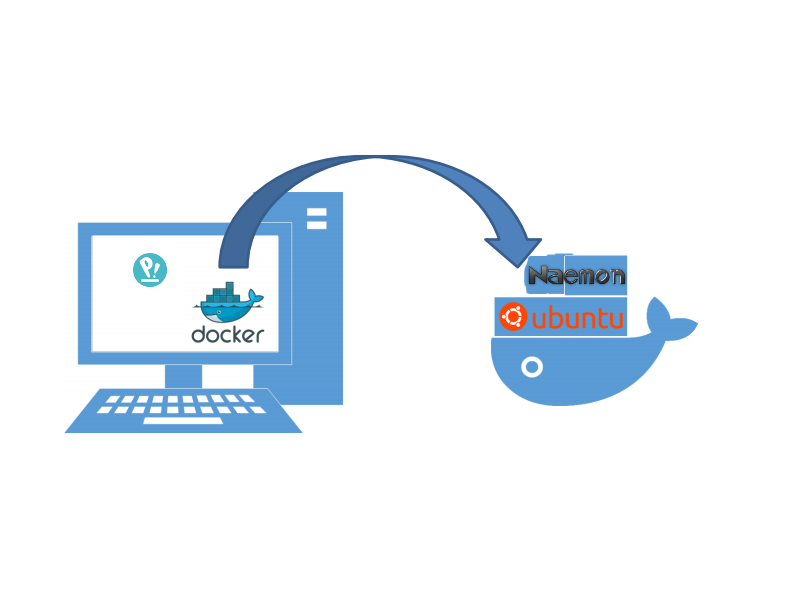
\includegraphics[width=0.9\textwidth]{imagenes/despliegue_naemon/docker_naemon.png}
	\caption{Estructura del contendor Docker con Naemon y Ubuntu de forma minimalista} \label{dockernaemon}
\end{figure}
\newpage
\section{Creación de Dockerfile}

Para poder realizar el despliegue tendremos que crear el fichero \textbf{Dockerfile}. Con este fichero construiremos la imagen de Naemon de forma automática, leyendo las instrucciones que le indiquemos.

Se trata de un documento de texto que contiene todas las órdenes a las que un usuario dado puede llamar, desde la línea de comandos, para crear una imagen.

Los pasos principales para crear una imagen a partir de un fichero Dockerfile son:

\begin{itemize}
	\item Crear un nuevo directorio que contenga el fichero, con el guión y otros ficheros que fuesen necesarios para crear la imagen.
	\item Crear el contenido.
	\item Construir la imagen mediante el comando docker build.
\end{itemize}

La sintaxis para el comando es:

\begin{lstlisting}[language=bash]
$ docker build [opciones] RUTA | URL | -
\end{lstlisting}


Las opciones más comunes son:
\begin{itemize}
	\item \textbf{-t}, nombre [:etiqueta]. Crea una imagen con el nombre y la etiqueta especificada a partir de las instrucciones indicadas en el fichero. Se recomienda usar este parámetro cuando se quiere asingar un nombre a la imagen.
	\item \textbf{–no-cache}. Por defecto, Docker guarda en memoria caché las acciones realizadas recientemente. Si se diese el caso de que ejecutamos un docker build varias veces, Docker comprobará si el fichero contiene las mismas instrucciones y, en caso afirmativo, no generará una nueva imagen. Para generar una nueva imagen omitiendo la memoria caché utilizaremos siempre esta opción.
	\item \textbf{–pull}. También por defecto. Docker solo descargará la imagen especificada en la expresión FROM si no existe. Para forzar que descargue la nueva versión de la imagen utilizaremos esta opción.
	\item \textbf{–quiet}. Por defecto, se muestra todo el proceso de creación, los comandos ejecutados y su salida. Utilizando esta opción solo mostrará el identificador de la imagen creada.
\end{itemize}

\begin{figure}[H]
	\centering
	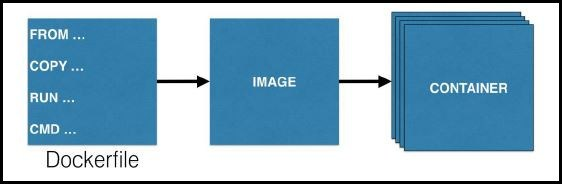
\includegraphics[width=0.9\textwidth]{imagenes/despliegue_naemon/dockerfile-image.png}
	\caption{Estructura de un fichero Dockerfile} \label{dockerfile}
\end{figure}
Para crear este fichero \textbf{Dockerfile} como el figurado en \ref{dockerfile} antes tenemos que aprender los comandos disponibles:
\begin{itemize}
	\item \textbf{MAINTAINER} : Nos permite configurar datos del autor, principalmente su nombre y su dirección de correo electrónico.
	\item \textbf{ENV} : Configura las variables de entorno.
	\item  \textbf{ADD} : Esta instrucción se encarga de copiar los ficheros y directorios desde una ubicación especificada y los agrega al sistema de ficheros del contenedor. Si se trata de añadir un fichero comprimido, al ejecutarse el guión lo descomprimirá de manera automática.
	\item  \textbf{COPY} : Es la expresión recomendada para copiar ficheros, similar a ADD.
	\item  \textbf{EXPOSE} : Indica los puertos en los que va a escuchar el contenedor. Hay que tener en cuenta que esta opción no consigue que los puertos sean accesibles desde el host; para esto debemos utilizar la exposición de puertos mediante la opción -p de docker run, tal y como explicamos en un artículo anterior.
	\item  \textbf{VOLUME} : Esta es una opción que muchos usuarios de la Web estaban esperando como agua de mayo. Nos permite utilizar en el contenedor una ubicación de nuestro host, y así, poder almacenar datos de manera permanente. Los volúmenes de los contenedores siempre son accesibles en el host anfitrión, en la ubicación: \textbf{/var/lib/docker/volumes/}
	\item  \textbf{WORKDIR} : El directorio por defecto donde ejecutaremos las acciones.
	\item  \textbf{USER} : Por defecto, todas las acciones son realizadas por el usuario root. Aquí podemos indicar un usuario diferente.
	\item  \textbf{SHELL} : En los contenedores, el punto de entrada es el comando \textbf{/bins/sh -c} para ejecutar los comandos específicos en CMD, o los comandos especificados en línea de comandos para la acción run.
	\item  \textbf{ARG} : Podemos añadir parámetros a nuestro Dockerfile para distintos propósitos.
\end{itemize}
A continuación indicaremos los pasos a seguir para instalar Naemon y la forma en que se ha indicado en dicho \textbf{Dockerfile}.
\subsection{Instalación de imagen base phusion}
La base de descarga será la siguiente \url{https://github.com/phusion/baseimage-docker}, donde podemos encontrar que dicha base es más eficiente que las bases comunes de Docker conocidas como \textbf{Alpine} y \textbf{BusyBox} en cuanto a la entrada y salida de sus datos de red. 
\begin{figure}[H]
	\centering
	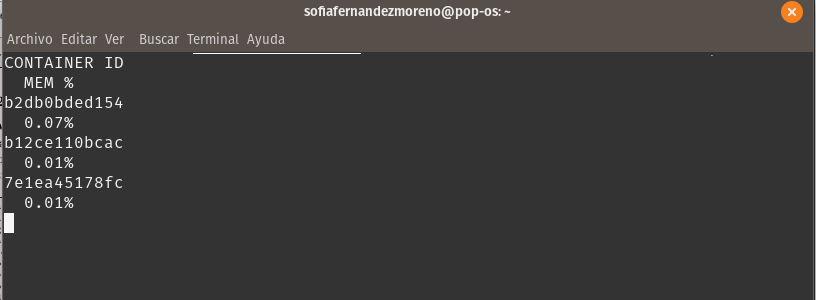
\includegraphics[width=0.9\textwidth]{imagenes/despliegue_naemon/estadisticasRAM.png}
	\caption{Comparativas de estadísticas} \label{phusion}
\end{figure}
En la figura \ref{phusion} se referencia al nombre \textbf{hungry\_poitras} con la imagen de la base de \textbf{phusion}, el nombre de \textbf{vigorous\_wing} con \textbf{Busybox} y \textbf{objective\_crazy} con \textbf{Alpine}.
\newpage
Por lo que tendremos que añadir en el Dockerfile las siguientes líneas:
\begin{lstlisting}[language=bash]
FROM phusion/baseimage:0.11
MAINTAINER Sofia <chui274@gmail.com>
\end{lstlisting}
\subsection{Instalación paquetes}
Debemos instalar las dependencias y los paquetes para que Naemon se pueda ejecutar perfectamente. Para ello debemos instalar el entorno LAMP en donde vayamos a aplicar Naemon. El comando que introduciremos en nuestro Dockerfile será el siguiente:
\begin{lstlisting}[language=bash]
RUN apt-get update && \
DEBIAN_FRONTEND=noninteractive \
apt-get install -y \
apache2\
apache2-utils\
libapache2-mod-fcgid\
libfontconfig1\
libjpeg62\
libgd3\
libxpm4\
xvfb\
ssmtp\
ruby\
python2.7\
python-boto\
perl\
libwww-perl\
libcrypt-ssleay-perl
\end{lstlisting}

Al principio le hemos indicado actualizar los repositorios por si existe alguna versión reciente en nuestro sistema.

Además hemos indicado para usar la sentencia siguiente:
\begin{lstlisting}[language=bash]
DEBIAN_FRONTEND=noninteractive
\end{lstlisting}
para indicar que queremos instalar y establecer el entorno apt-get de forma no interactivo y usar el script de shell en Dockerfile.
\newpage
\subsection{Instalación clave GPG}
El siguiente paso a seguir es agregar el repositorio de \textbf{Consol Labs} para crear la base de datos apt. Para ello debemos importar la clave GPG y así seguidamente generaremos las claves públicas para los servidores.

Por lo que habrá que añadir al documento \textbf{Dockerfile} las siguientes líneas para realizar lo anterior especificado:

\begin{lstlisting}[language=bash]
RUN   curl -s "https://labs.consol.de/repo/stable/RPM-GPG-KEY" | apt-key add -
RUN   gpg --keyserver keys.gnupg.net --recv-keys F8C1CA08A57B9ED7
RUN   gpg --armor --export F8C1CA08A57B9ED7 | apt-key add -
RUN   echo "deb http://labs.consol.de/repo/stable/ubuntu $(lsb_release -cs) main" > /etc/apt/sources.list.d/labs-consol-stable.list

\end{lstlisting}
\subsection{Instalación repositorio}
Realizado la instalación de la clave GPG debemos actualizar los repositorios y una vez actualizados los repositorios instalaremos la aplicación Naemon, además de que instalaremos los plugins correspondientes de Nagios que son compatibles con este, para ello introduciremos los siguientes comandos al Dockerfile:


\begin{lstlisting}[language=bash]

RUN apt-get update &&\
DEBIAN_FRONTEND=noninteractive apt-get install -y \
nagios-nrpe-plugin\
naemon=1.0.10


\end{lstlisting}

Le volvemos a indicar que queremos el entorno de forma no interactiva, además a la hora de realizar las instalaciones se le indicará, a través del \textbf{parámetro -y}, que confirmamos la instalación, ya que si no se confirma con anterioridad no realizará la creación de la imagen ya que no Docker no ofrece los permisos suficientes.

\subsection{Inicialización de directorios}
Una vez finalizada la instalación de Naemon, tendremos que indicar los directorios en los que vamos a trabajar, ya que el usuario desconoce los directorios internos de Naemon, para ello realizaremos la inicialización del directorio de datos creando unas variables de entorno. 
\newpage
Para ello crearemos un archivo llamado \textbf{data\_dirs.env} donde se recorrerá la variable global \textbf{DATA\_DIRS} que se compondrá de los directorios que queremos tener en nuestro contenedor, es decir, para poder tener acceso a los directorios con los que vamos a trabajar.

Dicho archivo .env permite personalizar las variables de entorno de trabajo individuales. Como hemos mencionado recorreremos la variable  \textbf{DATA\_DIRS} ingresando los directorios:

\begin{itemize}
	\item /etc/naemon
	\item /var/log/naemon
	\item /etc/thruk
	\item /var/log/thruk
	\item /usr/lib/naemon/plugins
\end{itemize}

Introduciremos dentro de la variable para agregar también el directorio de instalación de Thruk.

La forma de ir introduciendo los directorios lo haremos a través de forma de lenguaje bash de la siguiente manera:

\begin{lstlisting}[language=bash]
i=0
DATA_DIRS[((i++))]="/etc/naemon"
DATA_DIRS[((i++))]="/var/log/naemon"
DATA_DIRS[((i++))]="/etc/thruk"
DATA_DIRS[((i++))]="/var/log/thruk"
DATA_DIRS[((i++))]="/var/www"
DATA_DIRS[((i++))]="/usr/lib/naemon/plugins"
export DATA_DIRS


\end{lstlisting}

\subsubsection{Creación script de inicialización: init.bash}
Ahora una vez creada la variable de entorno con la que vamos a trabajar para poder operar con los directorios necesitamos inicializar el diseño del directorio de datos personalizado, para ello crearemos un script bash donde nos encargaremos de incluir en una variable \textbf{\textit{datadir}} todos los datos recogidos de la variable de entorno y moverlos a la plantilla de cada directorio, seguidamente realizaremos un enlace simbólico entre los directorios creados y los directorios reales.
\newpage
Es decir, a través del fichero \textbf{data\_dirs.env} accederemos a la variable de entorno \textbf{DATA\_DIRS} y por cada iteración del mismo moveremos dichas rutas a una plantilla y luego como hemos mencionado se creará el enlace simbólico.

El script es el siguiente:

\begin{lstlisting}[language=bash]
#!/bin/bash

source /data_dirs.env

mkdir -p /data
for datadir in "${DATA_DIRS[@]}"; do
mv ${datadir} ${datadir}-template
ln -s /data/${datadir#/*} ${datadir}
done

\end{lstlisting}
\subsubsection{Copia de archivos}
A través de Dockerfile y con el comando ADD copiaremos los archivos anteriores data\_dirs.env e init.bash a sus repestivos, es decir, realizaremos lo siguiente:
\begin{lstlisting}[language=bash]
ADD data_dirs.env /data_dirs.env
ADD init.bash /init.bash
\end{lstlisting}
Con esto queremos copiar el contenido de data\_dirs.env en el nuevo archivo /data\_dirs.env, al igual pasa con init.bash que copiaremos su contenido en la raíz del contenedor, es decir, en /init.bash.

Esto lo realizaremos para que el \textbf{Dockerfile pueda tener acceso a dichos datos y así poder operar}, ya que por defecto Docker no sabe de la existencia de dichos archivos sino los introducimos en el contenedor.

\subsubsection{Asignación de permisos}
Para poder ejecutar dicho script init.bash es necesario asignar una serie de permisos, para ello le indicaremos que queremos asignarle el permiso 755, es decir, este permiso se ocupa de que el propietario del fichero pueda leer, escribir y ejecutar el archivo. Todos los otros puedan leer y ejecutar el archivo. Este ajuste es común para los programas que son utilizados por todos los usuarios.
\newpage
Además le indicaremos también a través del comando sync que fuerce la grabación de los datos de la caché y así solventar la presencia de errores y reducir el tamaño de procesamiento.
Esto lo indicaremos en el fichero Dockerfile de la siguiente forma:
\begin{lstlisting}[language=bash]
RUN chmod 755 /init.bash &&\
sync && /init.bash &&\
sync && rm /init.bash
\end{lstlisting}

Además le indicaremos que ejecute el script init.bash para poder inicializar la información de los directorios.

\subsection{Cargar datos en carpeta raíz}
Como se mencionó anteriormente se creaba el directorio \textbf{data}, entonces para poder trabajar con el contenedor estableceremos el punto de montaje de Naemon en dicho directorio eso lo realizaremos con el comando \textbf{VOLUME} de Docker, que básicamente creará un punto de montaje con el nombre especificado y lo marca como que contiene volúmenes montados externamente desde el host nativo u otros contenedores.

 El valor puede ser una \textbf{\textit{matriz JSON}}, por ejemplo,\textbf{ VOLUME [``/var/log/"]} o una cadena simple con varios argumentos, como \textbf{VOLUME /var/logo}.
Cuando realicemos el comando \textbf{\textit{run}} de Docker, se inicializará el volumen recién creado con cualquier dato que exista en la ubicación especificada dentro de la imagen base.
Por lo tanto esto lo realizaremos en el fichero Dockerfile de la siguiente manera:
\begin{lstlisting}[language=bash]
VOLUME ["/data"]
\end{lstlisting}
\subsection{Protocolo de salida}
Para poder utilizar Naemon en un servidor web debemos realizar una conexión a través de los nodos y para ello utilizaremos el protocolo \textbf{TCP} desde el puerto 80 de HTTP.

Esto se podrá realizar a través de EXPOSE, qu su función es la de informar a Docker que el contenedor escucha en los puertos de red especificados en el tiempo de ejecución. Puede especificar si el puerto escucha en TCP o UDP, y el valor predeterminado es TCP si no se especifica el protocolo.
\newpage
Dicha instrucción no publica realmente el puerto. Funciona como un tipo de documentación entre la persona que construye la imagen y la persona que ejecuta el contenedor, acerca de los puertos que deben publicarse.

Para publicar realmente el puerto cuando se ejecuta el contenedor, se debe usar el flag \textbf{-p} en el comando docker run para publicar y asignar uno o más puertos, o el flag \textbf{-P} para publicar todos los puertos expuestos y asignarlos a puertos de alto orden.

Por defecto, EXPOSE asume TCP. También puede especificar UDP. En nuestro Dockerfile usaremos la siguiente línea para comunicar con TCP.

\begin{lstlisting}[language=bash]
EXPOSE 80/tcp
\end{lstlisting}
\subsection{Creación de imagen y ejecución de Dockerfile}
En esta sección especificaremos como podemos ejecutar a través de los propios comandos de Docker nuestra imagen, para ello realizaremos los siguientes pasos:
\subsubsection{Creación de ENTRYPOINT}
Primero utilizaremos el comando ENTRYPOINT en nuestro Dockerfile, ya que la funcionalidad de este es permitir configurar un contenedor que se ejecutará como un tipo de ejecutable. ENTRYPOINT puede tener dos formas:
\begin{itemize}
	\item \textbf{ENTRYPOINT [ejecutable,parametro]} Formato ejecutable
	\item \textbf{ENTRYPOINT comando parametro} Formato shell
\end{itemize}	
En nuestro caso se ha elegido la primera opción, ya que previamente hemos creado un fichero bash donde realizaremos las ejecuciones que contaremos a continuación. Previamente se ha creado en el Dockerfile las líneas para copiar dicho bash en la raíz del contenedor y darle la asignación de permisos de tipo 755 a dicho bash:
\begin{lstlisting}[language=bash]
ADD run.bash /run.bash
RUN chmod 755 /run.bash
\end{lstlisting}
\newpage
\paragraph{Fichero bash de ejecución: run.bash}

Anteriormente ejecutábamos la asignación de permisos de ejecución del fichero run.bash, para realizar la ejecución realizamos:
\begin{lstlisting}[language=bash]
ENTRYPOINT ["/run.bash"]
\end{lstlisting}

Con esto ejecutará dicho fichero bash que vamos a comentar a continuación:

Primero realizaremos la configuración de Naemon de forma externa a través del volumen \textbf{/data}
\begin{lstlisting}[language=bash]

source /data_dirs.env
DATA_PATH=/data

for datadir in "${DATA_DIRS[@]}"; do
	if [ ! -e "${DATA_PATH}/${datadir#/*}" ]
	then
		echo "Installing ${datadir}"
		mkdir -p ${DATA_PATH}/${datadir#/*}
		if [ "$(ls -A ${datadir}-template 2> /dev/null)"  ]
		then
			cp -pr ${datadir}-template/* ${DATA_PATH}/${datadir#/*}/
		fi
	fi
done

\end{lstlisting}

Para ello recorremos cada una de las instancias del volumen e iremos creando los directorios, solo si no existe el directorio. Seguido comprobamos que no exista un enlace simbólico, si de verdad no existe, copiaremos el contenido del directorio template dentro del directorio datadir.

En versiones antiguas de Naemon la contraseña del archivo htpasswd de thruk se guardaba en el archivo /etc/naemon, a través de nuestro script run comprobaremos que si es una versión antigua y se encuentra en dicha carpeta lo traslade al archivo /etc/thruk/htpasswd.

\begin{lstlisting}[language=bash]
if [ -e /etc/naemon/htpasswd ]
then
echo "UPGRADE: Moving the htpasswd file to the new location..."
mv /etc/naemon/htpasswd /etc/thruk/htpasswd
# We assume the naemon password was set in an upgrade situation
touch /etc/thruk/._install_script_password_set
fi
\end{lstlisting}

Por defecto se asigna el usuario y contraseña \textbf{thrukadmin} dentro del fichero /etc/thruk/htpasswd.
\newpage
Si no queremos que esa sea la contraseña asignada, podemos crear dentro del script una combinación para crear una contraseña aleatoria, para ello usaremos la variable RANDOM\_PASS y WEB\_ADMIN\_PASSWORD donde se asignará dicha contraseña.

A través de la siguientes líneas realizaremos lo comentado:


\begin{lstlisting}[language=bash]
RANDOM_PASS=`date +%s | md5sum | base64 | head -c 8`
WEB_ADMIN_PASSWORD=${WEB_ADMIN_PASSWORD:-$RANDOM_PASS}
htpasswd -bc /etc/thruk/htpasswd thrukadmin ${WEB_ADMIN_PASSWORD}
echo "Set the thrukadmin password to: $WEB_ADMIN_PASSWORD"
touch /etc/thruk/._install_script_password_set
\end{lstlisting}


Ahora nos encargaremos de comprobar que si estamos actualizando desde un contenedor anterior, moveremos el archivo llamado \textbf{cgi.cfg} a una nueva localización. Es decir, moveremos desde la ruta /etc/naemon/cgi.cfg a /etc/thruk/cgi.cfg.

A continuación se creará una función para realizar la parada del servidor apache y matar el proceso Naemon.

Realizamos por tanto lo siguiente:

\begin{lstlisting}[language=bash]
function salida_exitosa(){
/etc/init.d/apache2 stop
pkill naemon
exit $1
}
\end{lstlisting}

Hay que señalar que la imagen de phusion no funciona el comando \textbf{service naemon stop} por lo que habrá que realizar lo anterior.

Ahora nos aseguramos de dar los permisos de propiedad al volumen creado, es decir, a \textbf{data}, incluso si se cambian los UID o GID.

\begin{lstlisting}[language=bash]
chown -R naemon:naemon /data/etc/naemon /data/var/log/naemon
chown -R www-data:www-data /data/var/log/thruk /data/etc/thruk
\end{lstlisting}


Asignamos el permiso 775 al directorio /var/cache/naemon ya que no es editable por otros usuarios que no sean naemon, lo que significa que la herramienta de configuración de thruk no puede escribir en el directorio para verificaciones de configuración.

\begin{lstlisting}[language=bash]
chmod 775 /var/cache/naemon
\end{lstlisting}
\newpage
Solo nos quedará iniciar los servicios de Naemon y Apache con:

\begin{lstlisting}[language=bash]
service naemon start
service apache2 start
\end{lstlisting}

Anteriormente habíamos realizado una función para realizar una salida exitosa, ahora haremos uso de dicha función comprobando si naemon o apache está funcionando o no:
\begin{lstlisting}[language=bash]
trap "salida_exitosa 0;" SIGINT SIGTERM

while true
do
service naemon status > /dev/null
if (( $? != 0 ))
then
echo "Naemon no longer running"
salida_exitosa 1
fi

/etc/init.d/apache2 status > /dev/null
if (( $? != 0 ))
then
echo "Apache no longer running"
salida_exitosa 2
fi
sleep 1
done
\end{lstlisting}


El comando \textbf{trap} se usa para especificar las acciones a realizar cuando se reciban las señales.

Con todo esto ya estaría nuestro script listo solo para realizar la construcción de nuestra imagen.

\subsubsection{Creación de imagen a través de docker build}
Una vez tengamos la forma de realizar la correspondiente ejecución pasaremos a ejecutar su comando correspondiente en \textbf{Docker} para crear la imagen con todo lo anterior explicado. Para ello a través de terminal estableceremos el siguiente comando:
\begin{lstlisting}[language=bash]
$ docker build -t chui274/naemontfg .
\end{lstlisting}
\newpage
A la hora de crear la imagen indicaremos que se introduzca todo el contenido que hay en la raíz a través del . y con la opción -t indicaremos que queremos etiquetar la imagen con el nombre naemontfg con el usuario chui274 correspondiente, es decir, se creará un repositorio con el nombre chui274/naemontfg. Podemos asignarle el nombre que queramos al repositorio creado.
\subsubsection{Ejecución de imagen}
Para ejecutar la imagen creada solo tendremos que ejecutar el comando \textbf{docker run}. 
Para ello realizaremos la siguiente combinación de parámetros:
\begin{lstlisting}[language=bash]
$ docker run --rm -it -p 80:80/tcp chui274/naemontfg
\end{lstlisting}
Donde le indicaremos con los parámetros asociados lo siguiente:
\begin{itemize}
	\item \textbf{--rm} con esto hacemos que si existe el contenedor automáticamente lo borra.
	\item \textbf{-it} Permite el uso interactivo del contenedor.
	\item \textbf{-p} Aplica un puerto de escucha(en este caso se trata del puerto 80 a través de comunicación TCP)
\end{itemize}
\newpage
Si accedemos a través del navegador a la dirección \url{http://localhost:80} accederemos a la interfaz de \textbf{Thruk} como sigue:
\begin{figure}[H]
	\centering
	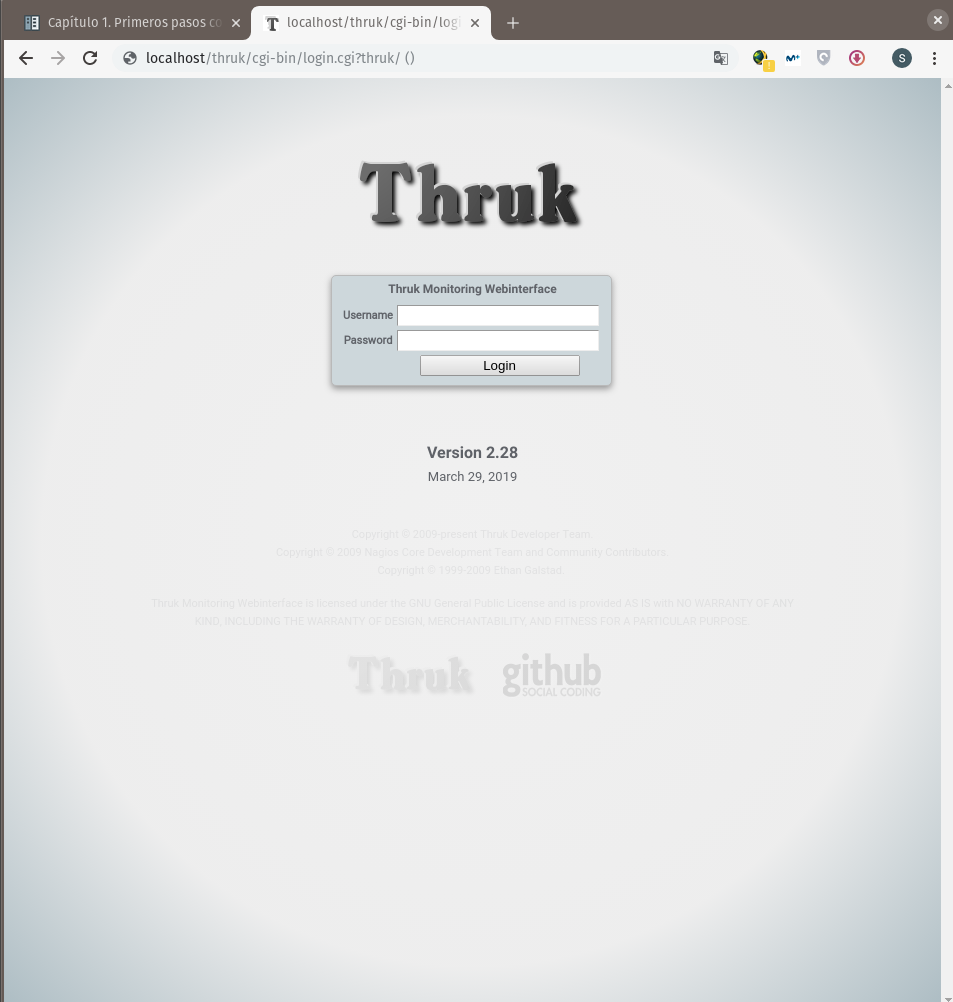
\includegraphics[width=0.7\textwidth]{imagenes/despliegue_naemon/ejecucionDocker.png}
	\caption{Ejecución de Docker} \label{run}
\end{figure}

\section{Orquestación de aplicaciones}

Existen múltiples definiciones sobre el concepto de \textbf{orquestación de aplicaciones} pero de un modo simple, podemos definir la \textbf{orquestación de servicios o aplicaciones} como el uso de la automatización para la creación y composición de la arquitectura, herramientas y procesos utilizados por operadores humanos para entregar un servicio.

La \textbf{orquestación} aprovecha tareas automatizadas y procesos predefinidos para permitir la creación de infraestructura complejas y para conseguir el aprovechamiento de los recursos de forma óptima y automatizada. Podemos considerar, a modo de analogía, el concepto de orquestación como un
proceso y la automatización como una tarea.
\newpage
De este modo, el objetivo principal de la orquestación consiste en la automatización de procesos orientados al despliegue y ciclo de vida de las aplicaciones o servicios. Y la automatización de procesos en los despliegues software se basan en el uso de algún tipo de software que facilite la instalación, configuración y mantenimiento del servicio o aplicación con la mínima intervención humana.

Existen dos tipos distintos de \textbf{orquestación} en base fundamentalmente a como se gestiona el escalado de recursos.
\begin{itemize}
	\item \textbf{Orquestación estática}: El sistema requiere una configuración más manual de los recursos y no permite el escalado de forma muy eficiente.
	\item \textbf{Orquestación Dinámica}: Escala de forma sencilla y eficientes los recursos de las aplicaciones y servicios y el propio sistema toma ciertas decisiones de forma automática.
\end{itemize}

En este proyecto, se plantea una solución de \textbf{orquestación estática} a través de la herramienta que cuenta Docker, llamada \textbf{Docker Compose} que permite la orquestación estática orientada a un funcionamiento más centrado un solo servidor, esta nos permite a través de un \textbf{fichero YML}, la definición y ejecución de aplicaciones Docker en múltiples contenedores.

Antes de comenzar con la explicación de \textbf{Docker Compose} explicaremos que es el formato \textbf{YML} o más bien conocido como \textbf{YAML} (Yet Another Markup Language). \cite{YML}

\textbf{YAML} se trata de un formato de serialización de datos de forma que sea legible para el usuario. Se inspira en lenguajes como XML, C, Python, Perl. Normalmente lo encontraremos con la extensión \textbf{.yml} o incluso \textbf{.yaml}.
\begin{figure}[H]
	\centering
	
\includegraphics[width=0.2\textwidth]{imagenes/despliegue_naemon/yaml.png}
	\caption{Logo de YAML} \label{yml}
\end{figure}
\newpage
Existen unas \textbf{reglas} generales que deben cumplirse en un documento \textbf{YAML} las principales son las siguientes:
\begin{itemize}
	\item Los datos de un documento YAML deben ser legibles, imprimibles y utilizando caracteres Unicode, UTF-8 ó UTF-16.
	\item Los comentarios se realizan utilizando el carácter \# dentro de la línea que contiene el comentario.
	\item Los caracteres , y ; deben ir seguidos de un espacio en blanco. De esta forma, se podrán representar valores que queramos que tengan esos caracteres.
	\item Los espacios en blanco están permitidos, pero no los tabuladores.
	\item Las listas comienzan por el caracter \textbf{``–"} con un valor por cada línea, aunque también se pueden utilizar corchetes \textbf{[]} poniendo los valores dentro de ellos separados por comas \textbf{``,"}junto con un espacio en blanco.
	\item Un vector estará formado por el par \textbf{clave/valor}, estando separados ambos por \textbf{``:"} poniendo uno por línea, aunque también podemos utilizar \textbf{{}} poniendo cada uno de ellos dentro separados por comas \textbf{``,"} junto con un espacio en blanco.
	\item Se pueden utilizar caracteres de escape \ para representar caracteres especiales.
\end{itemize}

\subsection{Uso de Docker Compose}

Como se ha mencionado se utilizará dicha herramienta para la ejecución de varios contenedores de Naemon trabajando de forma distribuida, pudiendo crear e iniciar todos a la vez.

Para ello tenemos que definir un fichero Dockerfile, ya lo tenemos creado.
Seguidamente crearemos un archivo llamado \textbf{docker-compose.yml} que se encargará de las ejecuciones del entorno.

Y para finalizar y reproducir la ejecución solo será necesario introducir a través de terminal desde la ruta en la que se encuentra el archivo de Docker Compose introducir:

\begin{lstlisting}[language=bash]
$ docker-compose up
\end{lstlisting}
\newpage
A continuación se comenta lo introducido en dicho archivo docker-compose.yml:

\begin{lstlisting}[language=bash]
version: '3.7'
services:
naemon:
build: .

ports:
- "32768:80"
image: "chui274/naemontfg"


\end{lstlisting}

Con la etiqueta version especificaremos la versión de Compose e incluyendo la versión de Docker Engine, por lo que si asignamos \textbf{version: '3.7'} estamos indicando que queremos la versión 3.7 de Docker Compose y la versión 18.06.0+ de Docker Engine.

A través de la etiqueta services comenzaremos a definir los contenedores que queremos crear, comenzamos creando nuestro contenedor llamado naemon, para la construcción es necesario la etiqueta build.

La etiqueta \textbf{build}  indicará la imagen de Dockerfile que vamos a usar, le indicamos . para que lea desde el archivo Dockerfile que se encontrará en el directorio principal.

Le indicaremos a través de la etiqueta \textbf{ports}   que realiza la escucha de la interfaz de thruk a través del puerto 32768.

Ahora a través de la etiqueta \textbf{image}  si hemos realizado la construcción bien con build, cogeremos la imagen desde chui274/naemontfg, que ha sido construida desde \textbf{.} .

Realizando el comando anterior mencionado a través de terminal, tendremos lo siguiente:

\begin{figure}[H]
	\centering
	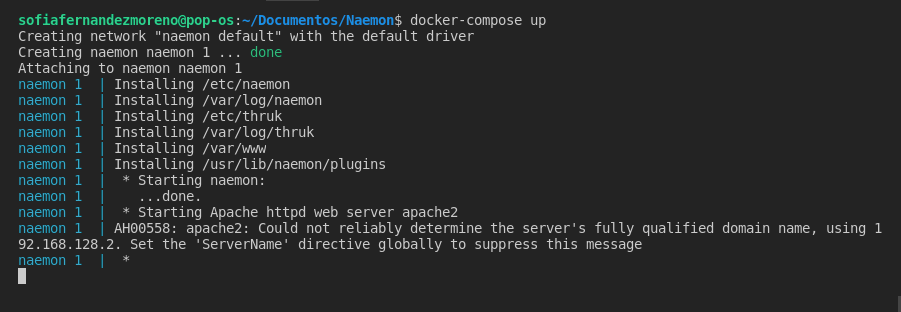
\includegraphics[width=1\textwidth]{imagenes/despliegue_naemon/terminal.png}
	\caption{Ejecución de Docker Compose} \label{dockercompose}
\end{figure}

Ahora estamos a disposición de probar la dirección \url{http://localhost:32768/} para acceder a Naemon a través de Thruk.

\begin{figure}[H]
	\centering
		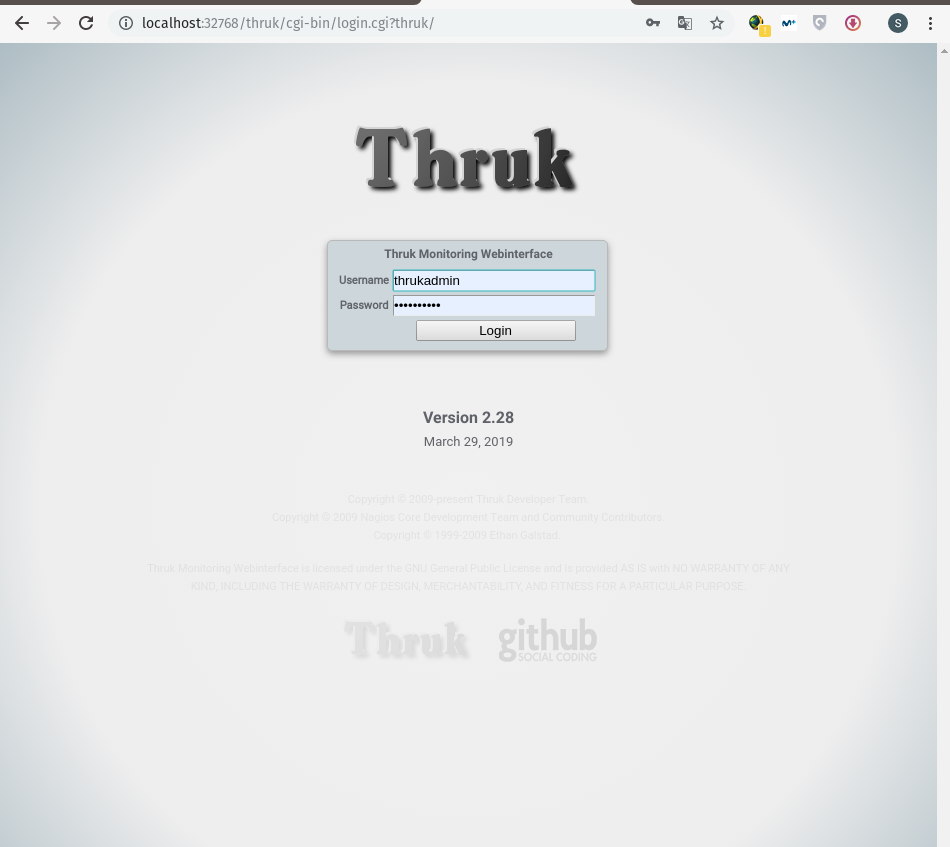
\includegraphics[width=1\textwidth]{imagenes/despliegue_naemon/pantallaDockerNaemon.png}
	\caption{Ejecución de Thruk mediante Docker Compose} \label{dockercomposethruk}
\end{figure}
\newpage

\chapter{Pruebas de carga} \label{ch:carga}
\section{Introducción}
A la hora de trabajar con un sistema a un nivel de rendimiento estable y bueno es fundamental que se realicen pruebas al comienzo del inicio del desarrollo de su software. Al igual que en las pruebas funcionales, el coste de solucionar defectos se ve aumentado conforme más se tarde en detectarlos.\cite{performingtest}

Para que las pruebas sean lo más fiables posible, el entorno de prueba debe ser lo más parecido posible al de producción.

Las \textbf{pruebas de rendimiento} son un conjunto de pruebas que nos permiten medir la velocidad de ejecución de una serie de tareas en un sistema, bajo unas condiciones determinadas.

Las \textbf{pruebas de rendimiento} sirven, entre otras cosas, para:
\begin{itemize}
	\item Demostrar que el sistema cumple los criterios de rendimiento.
	\item Validar y verificar atributos de la calidad del sistema: escalabilidad, fiabilidad, uso de los recursos.
	\item Comparar dos sistemas para saber cuál de ellos funciona mejor.
	\item Detectar cuellos de botella,es decir, medir qué partes del sistema o de carga de trabajo provocan que el conjunto rinda mal.
\end{itemize}
\newpage
\section{Tipos de pruebas de rendimiento}

Podemos encontrarnos con las siguientes pruebas a la hora de probar el rendimiento de un sistema:
\subsection{Prueba de carga}
Se trata de una prueba que generalmente observa el comportamiento de una aplicación bajo una serie de peticiones. 
Por ejemplo puede ser el número esperado de usuarios concurrentes, utilizando la aplicación que realizan un número específico de transacciones, durante el tiempo que dura la carga.

Esta prueba puede mostrar los tiempos de respuesta de todas las transacciones importantes de la aplicación. Si también se monitorizan otros aspectos como la base de datos, el servidor de aplicaciones, etc., entonces esta prueba puede mostrar el cuello de botella en la aplicación.\cite{pruebas}

\subsection{Prueba de estrés}

Se utiliza como su propio nombre dice estresar la aplicación, es decir, que se encuentre en un estado forzado. Se va aumentando el número de usuarios que se agregan a la aplicación y se ejecuta una prueba de carga hasta que se rompe. Este tipo de prueba se realiza para determinar la solidez de la aplicación en los momentos de carga extrema. Esto ayuda a los administradores para determinar si la aplicación rendirá lo suficiente en caso de que la carga real supere a la carga esperada.\cite{pruebas}

\subsection{Prueba de estabilidad (Soak Testing)}

Se realiza para determinar si la aplicación es capaz de aguantar una carga concreta. El objetivo principal de este tipo de pruebas es verificar que no existen fugas de memoria o procesos que pierdan rendimiento transcurrido un cierto periodo de tiempo.\cite{pruebas}
\newpage
\subsection{Prueba de pico (Spike Testing)}

En esta prueba, la aplicación se prueba con incrementos y decrementos extremos en la carga. Se realiza para estimar la debilidad de una aplicación.

Ayuda a evaluar el comportamiento del sistema de software en incrementos o disminuciones repentinos en la carga del usuario.\cite{pruebas}


\section{Tipo de prueba seleccionada}
Para este proyecto se ha elegido la opción de realizar pruebas de carga para poder simular el uso de concurrencia real en nuestro despliegue de Naemon.

Además usaremos este tipo de prueba puesto que queremos medir la \textbf{\textit{performance}} de un sitio web, el cual mencionaremos más adelante y este tipo de prueba nos será de gran utilidad.

A continuación se introducirán una serie de herramientas para poder simular este tipo de prueba de carga, donde finalmente se escogerá entre todas una concreta.
\subsubsection{Gatling}
Se trata de una herramienta de código abierto y multiplataforma, es decir, podremos utilizarlo en cualquier dispositivo, por lo que permite gran libertad en cuanto a su uso. Además, ofrece una gestión óptima de los recursos del sistema frente a otras herramientas como JMeter\cite{comparativeGatling}. Estas pruebas se pueden hacer sobre diversos protocolos como pueden ser HTTP (páginas web, servicios REST), FTP, sockets de web, etc.\cite{gatling}
\begin{figure}[H]
	\centering
	
\includegraphics[width=0.4\textwidth]{imagenes/carga/gatling.png}
	\caption{Gatling} \label{gatling}
\end{figure}
Las pruebas de \textbf{Gatling}  consistirán en simulaciones donde se realizarán flujos de uso de la web, y al final obtendremos un reporte detallado con los tiempos de respuesta, resultados de las peticiones, etc.

\subsubsection{Locust}

\textbf{Locust} \cite{locust} es una herramienta de prueba de carga de usuario distribuida y fácil de usar. Está diseñado para probar sitios web (u otros sistemas) y determinar cuántos usuarios concurrentes puede manejar un sistema.

La idea es que durante una prueba, un enjambre de langostas atacará el sitio web. El comportamiento de cada langosta (o usuario de prueba, si lo desea) se define por nuestra cuenta y el proceso de enjambre se supervisa desde una interfaz de usuario web en tiempo real. Esto ayudará a probar e identificar cuellos de botella en el código antes de permitir el ingreso de usuarios reales.
\begin{figure}[H]
	\centering
	
\includegraphics[width=0.4\textwidth]{imagenes/carga/locust.jpeg}
	\caption{Locust} \label{locust}
\end{figure}
Locust está completamente basado en eventos y, por lo tanto, es posible admitir miles de usuarios concurrentes en una sola máquina. A diferencia de muchas otras aplicaciones basadas en eventos, no usa devoluciones de llamadas. En cambio, usa procesos ligeros, a través de \textit{\textbf{gevent}}. Cada langosta pululando en su sitio se está ejecutando dentro de su propio proceso (o \textit{greenlet}, para ser correcto). Esto permite escribir escenarios muy expresivos en Python sin complicar su código con devoluciones de llamadas.
\newpage
\subsubsection{Jmeter}
\textbf{Apache JMeter} \cite{jmeter} es la única aplicación de escritorio en esta revisión. Tiene una interfaz gráfica de usuario fácil de usar, lo que hace que el desarrollo de pruebas y la depuración sean mucho más fáciles. Tiene una estructura modular, en la que el núcleo se extiende mediante complementos. Esto significa que todos los protocolos y características implementados son complementos que han sido desarrollados por Apache Software Foundation o colaboradores en línea.
\begin{figure}[H]
	\centering
	
\includegraphics[width=0.4\textwidth]{imagenes/carga/jmeter.png}
	\caption{JMeter} \label{jmeter}
\end{figure}
Tiene más funciones e integraciones, y también una base de usuarios más grande que cualquier otra herramienta de prueba de carga de código abierto.

El principal aspecto negativo de JMeter es que las configuraciones, incluida la lógica del escenario del usuario, están escritas en XML.

\subsection{Alternativa elegida: Locust}

Se ha elegido esta opción puesto que se trata de un programa multiplataforma por lo que podremos ejecutarlo en cualquier sistema operativo. Además de ofrecer una alta escalabilidad debido a la implementación que cuenta basada en eventos. Otra cosa a destacar, se trata de la escalabilidad en cuanto a la distribución de los agentes, permite incluir un número infinito de agentes. 

Locust es altamente escalable debido a su implementación totalmente basada en eventos. Debido a estos hechos, Locust tiene una comunidad en rápido crecimiento, que prefieren este marco en lugar de JMeter (siendo ésta de las más populares).

Cuenta con una interfaz de usuario de comando y control basada en web, además de soporte para la generación de carga distribuida, lo que lo hace ser más actualizable y seguro para el futuro.
\newpage
Permite además la descarga de los resultados en tipo CSV y JSON.

\section{Instalación de Locust}

Locust está disponible en \textbf{PyPI} y se puede instalar a través del comando pip.

\begin{lstlisting}[language=bash]
$ apt-get install python-pip
$ pip install locustio
\end{lstlisting}

\section{Funcionamiento de herramienta Locust}
Para poder empezar a trabajar en Locust es necesario tener activado un servidor web, que en este caso será \textbf{Apache}.
Una vez inicializado el servidor web de Apache, si no se encuentra activo podemos activarlo a través del comando:

\begin{lstlisting}[language=bash]
$ service apache2 start
\end{lstlisting}

Activado el servidor web, debemos ejecutar \textbf{Locust} en el servidor Web Apache, para ello debemos configurar un archivo \textbf{locustfile.py} que contará con el código necesario para realizar las pruebas de carga necesarias, distribuyendo la prueba de rendimiento en diferentes máquinas para que se pueda crear más carga en la aplicación.\cite{locustfile}

\section{Ejecución distribuida}

La ejecución de una sola máquina no es suficiente para modelar o simular una carga, por lo que Locust admite la ejecución de pruebas de carga distribuidas en múltiples máquinas.

Para hacer esto, se debe iniciar una instancia de Locust en modo maestro usando el flag --master. Dicha instancia será la ejecutada por la interfaz web de Locust, donde se inicia la prueba y se muestran las estadísticas en vivo.
\newpage
Para poder simular las cargas debemos de iniciar uno o varios nodos con el flag --slave para simular los esclavos, junto con el --master-host (especificando la IP o nombre del host del nodo maestro).

Una configuración común es ejecutar un solo maestro en una máquina, y luego ejecutar una instancia esclava por núcleo del procesador, en las máquinas esclavas.

Para poder establecer dicha configuración de forma automática a través del despliegue realizado en la tecnología \textbf{Docker}, debemos crear una nueva instancia dentro de nuestro archivo \textbf{docker-compose.yml}.

Para ello creamos las máquinas llamadas \textbf{locust-master y locust-worker} por las cuales queremos simular la carga maestro-esclavo a través de Docker.

En el archivo \textbf{docker-compose.yml} crearemos estas máquinas a través de la imagen \textbf{swernst/locusts}, la cual cuenta con la \textbf{última versión de Locust para Docker}, recogida del repositorio de \textbf{Docker Hub}. En esta imagen tendremos que la instancia del maestro se encarga de alojar una interfaz web, así como la coordinación con los esclavos. En este caso el esclavo se encargará de realizar los test y crear reportes de información al maestro de forma estadística.

Esta división permite escalar el número de esclavos para realizar pruebas de carga realmente grandes.

Ambas vinculan el directorio \textbf{scripts} en el contenedor a un subdirectorio en nuestra maquina host con el mismo nombre. Esto hará que nos permita eliminar los scripts que se quieran usar para dicha prueba y ponerlo a disposición de cualquier caso.

Tenemos que el servicio \textbf{locust-master} tiene un puerto definido, exactamente el puerto 8089, lo que hace que podamos tener acceso a la interfaz web de Locust desde ese servicio.
Además el servicio \textbf{locust-worker} está tomando un parámetro de comando adicional que le dice que se conecta a master para la orquestación, esto es a través de la línea: \textbf{command: "--master-host=locust-master"}.
\newpage
Esto redactado dentro de nuestro archivo \textbf{docker-compose.yml} quedará de la siguiente manera:
\begin{lstlisting}[language=bash]
  
locust-master:
image: swernst/locusts
volumes:
- ./scripts:/scripts
ports:
- "8089:8089"
depends_on:
- wordpress
locust-worker:
image: swernst/locusts
command: "--master-host=locust-master"
volumes:
- ./scripts:/scripts


\end{lstlisting}

Donde la línea establecida en locust-master como: 

\begin{lstlisting}[language=bash]
depends_on:
- wordpress
\end{lstlisting}

Viene indicada para la siguiente explicación donde trabajaremos con el sistema final establecido, el cual será en \textbf{WordPress}, donde también será creada un servicio a través del archivo \textbf{docker-compose}.

A la hora de lanzar esta ejecución en el cual tengamos tres instancias trabajando, o lo que es lo mismo tres esclavos, debemos ejecutar la siguiente línea para lanzar el contenedor Docker:

\begin{lstlisting}[language=bash]
$  docker-compose up --scale locust-worker=3 
\end{lstlisting}

O simplemente si queremos un maestro y un esclavo haríamos el levantamiento del contenedor de la siguiente manera:

\begin{lstlisting}[language=bash]
$  docker-compose up 
\end{lstlisting}
\newpage
\section{Configuración Locustfile}
\textbf{Locust} generará una hebra para cada usuario que está siendo simulado y cada usuario viene representado por una clase \textbf{locust}.
Para empezar con la configuración de nuestro archivo \textbf{locustfile.py},por el cual nos encargaremos de realizar las pruebas de carga correspondientes a nuestro sistema final, pero antes debemos explicar los atributos que vamos a utilizar para realizar estos test o pruebas:

\begin{itemize}
	\item \textbf{TaskSet}: se trata de una colección de tareas, es decir, define el comportamiento del usuario. Para cada acción definida debe definirse la anotación \textbf{@task}.
	\item \textbf{HttpLocust}: utilizada para cargar la prueba de rendimiento de un sistema en el servidor. Representa un usuario el cual será atacado y que será probado con carga. Dicha clase crea un atributo cliente que se trata del cliente HTTP que se encarga de realizar el enlace entre la sesión y las peticiones.
\end{itemize}

Un ejemplo de un test simple sería el siguiente:
\begin{lstlisting}[language=Python]
from locust import HttpLocust, TaskSet, task

class UserBehavior(TaskSet):
@task(2)
def root(self):
self.client.get('/')
@task(1)
def host(self):
self.client.get('/?p=1')
class WebsiteUser(HttpLocust):
task_set = UserBehavior
min_wait = 5000
max_wait = 9000

\end{lstlisting}

Donde se ha realizado la obtención de los datos de la página principal del sistema y también la obtención de los datos de un artículo concreto del sistema que en este caso ha sido WordPress.

Hay que especificar que en la clase Locust se permite especificar el tiempo de espera mínimo y máximo en milisegundos, por usuario simulador, entre la ejecución de las tareas, esto se realiza mediante las variables \textbf{min\_wait y max\_wait}.
\newpage
Cabe mencionar que de forma predeterminada, el tiempo se elige aleatoriamente  de forma uniforme entre dichas variables, pero se puede usar cualquier distribución de tiempo definida por el usuario configurando una variable \textbf{wait\_function} en cualquier función arbitraria. Podemos realizar como ejemplo un tiempo de espera distribuido de forma exponencial con un promedio de 1 segundo, esto en código Python se establece de la siguiente forma:
\begin{lstlisting}[language=Python]

class WebsiteUser(HttpLocust):
task_set = UserBehavior
wait_function = lambda self: random.expovariate(1)*1000

\end{lstlisting}

En el siguiente capítulo pondremos este archivo de configuración a prueba mediante el despliegue de un sistema WordPress, el cual monitorizar la generación de carga por parte de lo clientes y de cómo sirve la carga el sistema, además de modelar la carga a partir de los datos recopilados durante la monitorización.
\newpage
\chapter{Pruebas de carga en sistema} \label{ch:carga_cliente}

En este capítulo profundizaremos sobre la monitorización de un sistema, en este caso supondrá un sistema en \textbf{WordPress}, este se trata de un sistema de gestión de contenidos.

A través de la herramienta \textbf{Naemon} y el framework de \textbf{Locust} queremos realizar el análisis de dicho sistema.
\section{Despliegue de sistema a través del contenedor Docker}
Como se realizó en capítulos anteriores para realizar el despliegue de Naemon y Locust en Docker, esta vez pasaremos a la realización del despliegue de WordPress. Para ello nos basaremos en dos instancias separadas: \textbf{una instancia para Wordpress} y \textbf{otra instancia separada para MySQL con un volumen montado para la persistencia de los datos de MySql}.

En él definimos dos \textbf{servicios}: \textbf{db} (correspondiente a MySQL) y \textbf{wordpress}. En el \textbf{primer servicio (db)} indicamos la imagen que queremos descargarnos (un MySQL versión 5.7) y algunos parámetros de configuración. Los más relevantes son la redirección de puertos (del 8081 del anfitrión al 3306 del huésped) y parámetros de la base de datos en sí (usuario, contraseña, etc).
\newpage
El \textbf{segundo servicio es WordPress (wordpress)} y sigue un patrón parecido. Aquí, por ejemplo, indicamos que queremos usar el puerto 80 para acceder a nuestro WordPress. También especificamos que db es una dependencia de WordPress (este contenedor no puede funcionar sin el otro) esto lo haremos mediante la opción \textbf{depends on}. Y también indicamos parámetros adicionales como, por ejemplo, dónde está la base de datos y cómo acceder a ella. Todo esto vendrá definido en el archivo \textbf{docker-compose.yml} de la siguiente manera:
\begin{lstlisting}[language=bash]
db:
	image: mysql:5.7
	volumes:
	 - db_data:/var/lib/mysql
	restart: always
	environment:
		MYSQL_ROOT_PASSWORD: somewordpress
		MYSQL_DATABASE: wordpress
		MYSQL_USER: wordpress
		MYSQL_PASSWORD: wordpress

wordpress:
	depends_on:
	 - db
	image: wordpress:latest
	ports:
	 - "80:80"
	restart: always
	environment:
		WORDPRESS_DB_HOST: db:3306
		WORDPRESS_DB_USER: wordpress
		WORDPRESS_DB_PASSWORD: wordpress
		WORDPRESS_DB_NAME: wordpress
\end{lstlisting}
Si realizamos la puesta en marcha mediante el comando \textbf{docker-compose up} comenzará con la descarga de las imágenes de \textbf{WordPress y MySQL}, y de forma seguida pondrá en funcionamiento el sistema de \textbf{WordPress}.

Cuando termine la instalación del contenedor, accedemos al navegador e introducimos la siguiente dirección \url{http://localhost:80} o \url{http://localhost}, donde se lanzará la instalación correspondiente de \textbf{WordPress}.
\newpage
\begin{figure}[H]
	\centering
	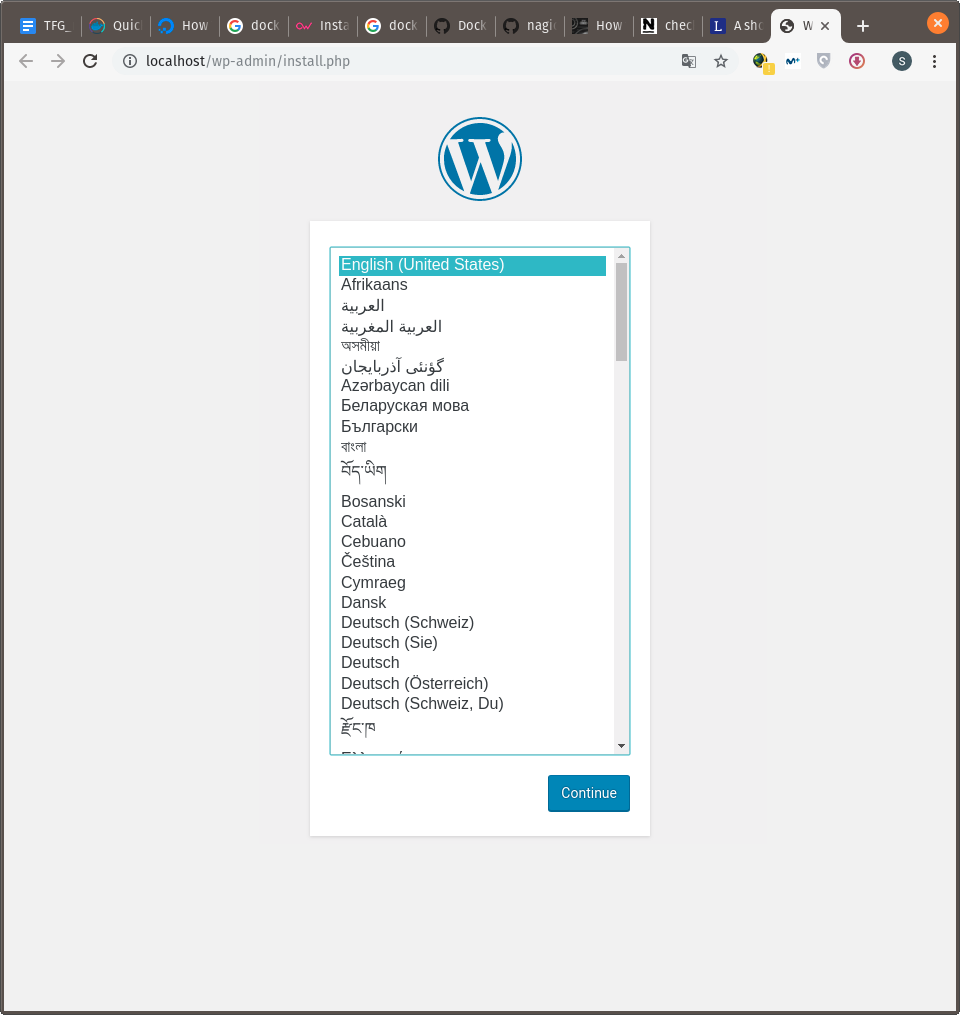
\includegraphics[scale=0.2]{imagenes/wordpress/wordpressinstall.png}
	\caption{Instalación de WordPress} \label{wordpress}
\end{figure}

Realizado este paso solo quedará instalar \textbf{WordPress} con el blog correspondiente que se quiera ejecutar, en este caso se ha llamado al blog \textbf{Monitorización TFG}:

\begin{figure}[H]
	\centering
	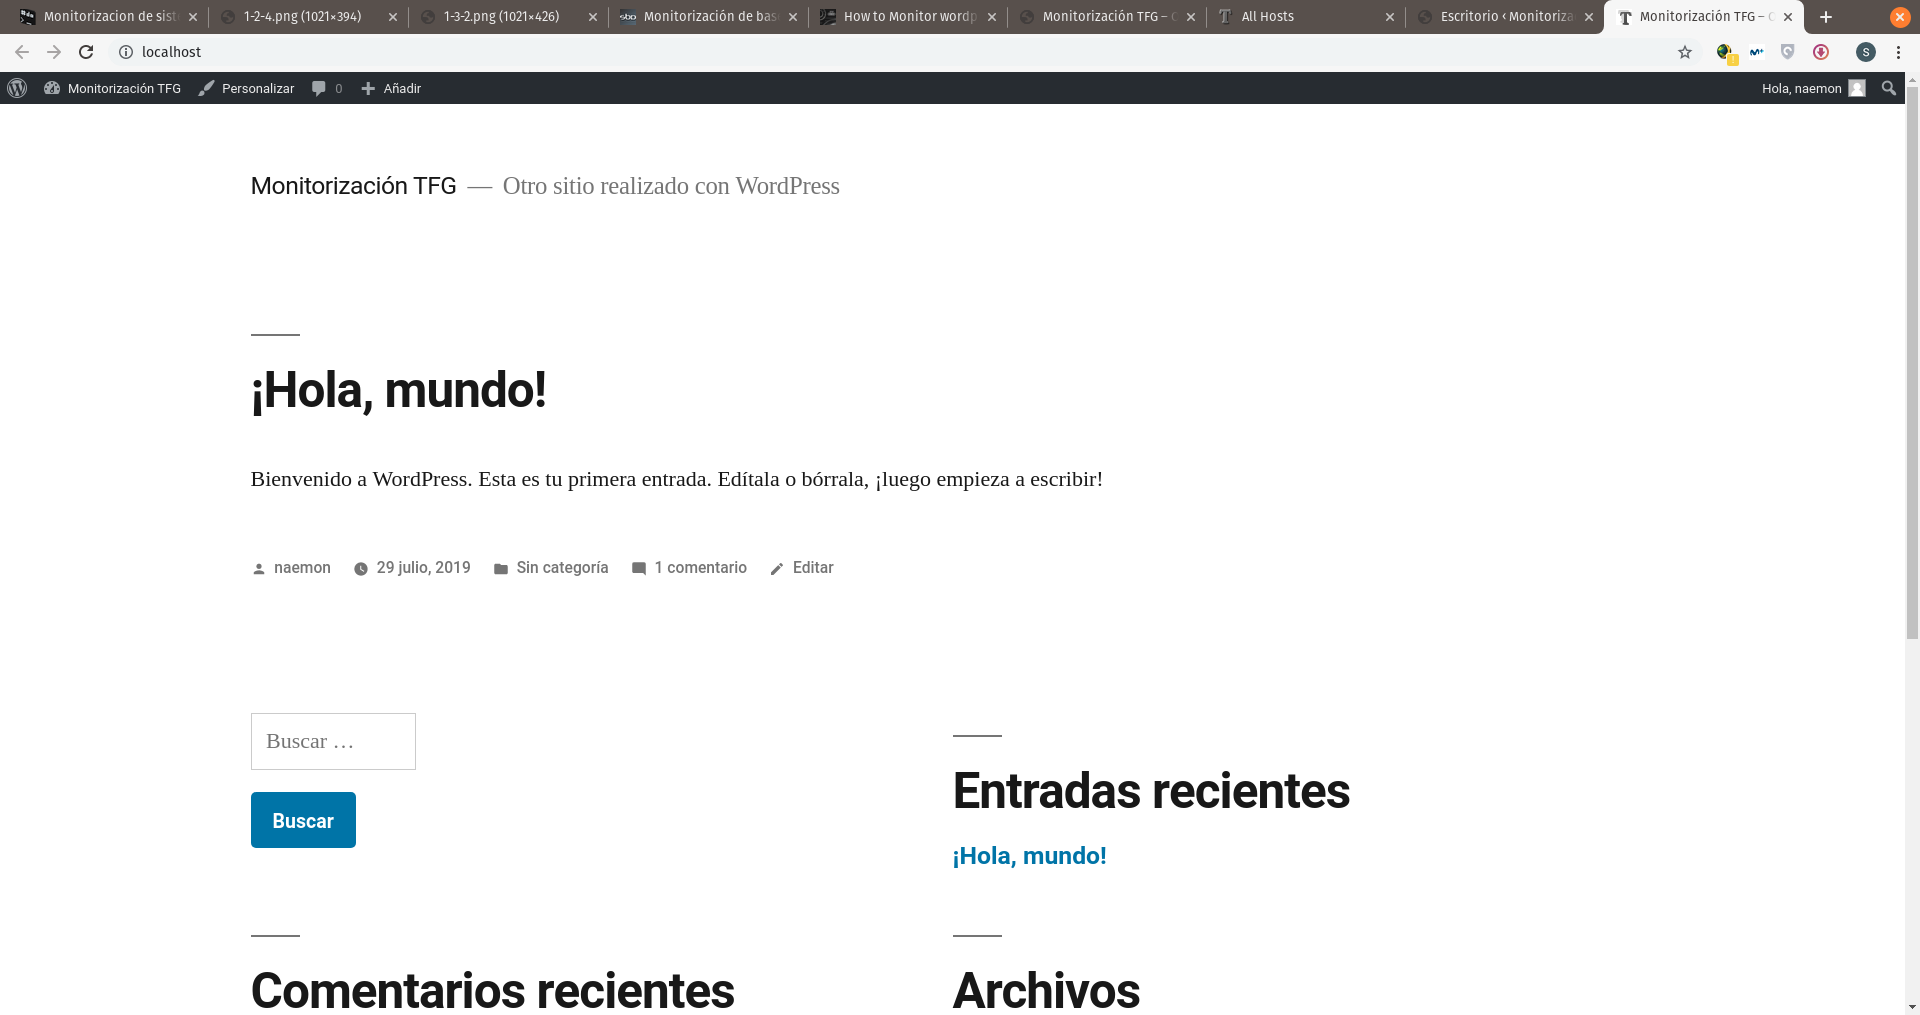
\includegraphics[scale=0.2]{imagenes/wordpress/instalacion-wordpress.png}
	\caption{Pantalla principal Blog de WordPress} \label{wordpress}
\end{figure}
\newpage
\section{Enlazado con Locust}
Como ya contamos con nuestro sistema montado sólo nos quedará realizar el enlazado con el \textbf{Framework de Locust}, para ello es necesario adaptar la configuración interna del archivo \textbf{locust.config.json}. Este archivo será añadido al fichero do\textbf{cker-compose.yml} junto al \textbf{locustfile.py}.

Dicho archivo nos servirá para especificar la \textbf{URL raíz de la API} a la que se va a redirigir la \textbf{API de Locust}, junto con la lista de nombres de clase para las subclases de Locust que se usarán en la prueba.

El archivo \textbf{JSON} que tendremos que crear será algo como el siguiente:

\begin{lstlisting}[language=json,firstnumber=1]
{
"target": "http://wordpress",
"locusts": ["WebsiteUser"]
}
\end{lstlisting}

Donde \textbf{target} corresponde a la dirección que vamos a capturar, especificamos  \url{http://wordpress} ya que wordpress coincide con la etiqueta de creación de la imagen de WordPress, se podría poner  \url{http://localhost} y funcionaría, pero esto garantiza que verdaderamente estamos estableciendo la relación con ese entorno, ya que a la hora de la realización se ha encontrado un problema con el paso de peticiones GET a través del servidor Apache y era necesario aplicar un cambio interno en la configuración de WordPress, estableciendo el puerto base como 80. Por lo que esta medida es garantizable y más rápida de realizar, ya que se está trabajando a través del despliegue de Docker.

La etiqueta \textbf{locusts} corresponde a la tarea o clase por la que vamos a ejecutar, en este caso es \textbf{WebsiteUser} que realiza toda la funcionalidad de nuestro archivo.
\newpage
\subsection{Creación de archivo Locustfile}

Como se realizó en capítulos anteriores para poder empezar a trabajar con \textbf{Locust} es necesario la creación del archivo \textbf{locustfile.py} para poder realizar las distintas pruebas de carga. Para ello analizaremos la prueba de carga a la hora de acceder y salir del sistema WordPress, además realizaremos una prueba de carga para un artículo concreto, esto se realizará mediante el lanzado de la petición \textbf{GET} hacia la URL \textbf{/?p=1}.

En el caso del \textbf{login} y el \textbf{logout}, lanzaremos peticiones \textbf{POST}, ya que éste tipo de petición se utiliza para enviar una entidad a un recurso en específico, causando a menudo un cambio en el estado o efectos secundarios en el servidor.

El código del archivo \textbf{locustfile.py} quedará de la siguiente manera:
\begin{lstlisting}[language=Python]
from locust import HttpLocust, TaskSet, task

def login(l):
l.client.post("/login", {"username":"naemon", "password":"naemon"})

def logout(l):
l.client.post("/logout", {"username":"naemon", "password":"naemon"})


class UserBehavior(TaskSet):
def on_start(self):
login(self)

def on_stop(self):
logout(self)
@task(2)
def root(self):
self.client.get('/')
@task(1)
def host(self):
self.client.get('/?p=1')
class WebsiteUser(HttpLocust):
task_set = UserBehavior
min_wait = 5000
max_wait = 9000


\end{lstlisting}

Si lanzamos en terminal el comando \textbf{docker-compose up} y lanzamos el enlace \url{http://localhost:8089/} ejecutaremos \textbf{Locust} a través del navegador.

También podemos especificar el número de instancias de esclavos a través del comando siguiente:
\begin{lstlisting}[language=bash]

$ docker-compose up --scale locust-worker=3

\end{lstlisting}
\newpage
\section{Pruebas de carga con sistema WordPress}
Una vez contamos con los dos archivos anteriormente mencionados, pasamos a la ejecución de la prueba de carga, para ello accedemos al enlace \url{http:localhost:8089} donde nos aparecerá la pantalla principal de \textbf{Locust} donde debemos especificar el \textbf{número de usuarios a simular (Number of users simulate) y el Hatch rate}. El valor de \textbf{Hatch rate} representa por cada segundo, cuántos usuarios se agregarán a los usuarios actuales hasta la cantidad total de usuarios. Cada hatch realizado Locust llama a la función \textbf{on\_start} si existe.\\

\begin{figure}[H]
	\centering
	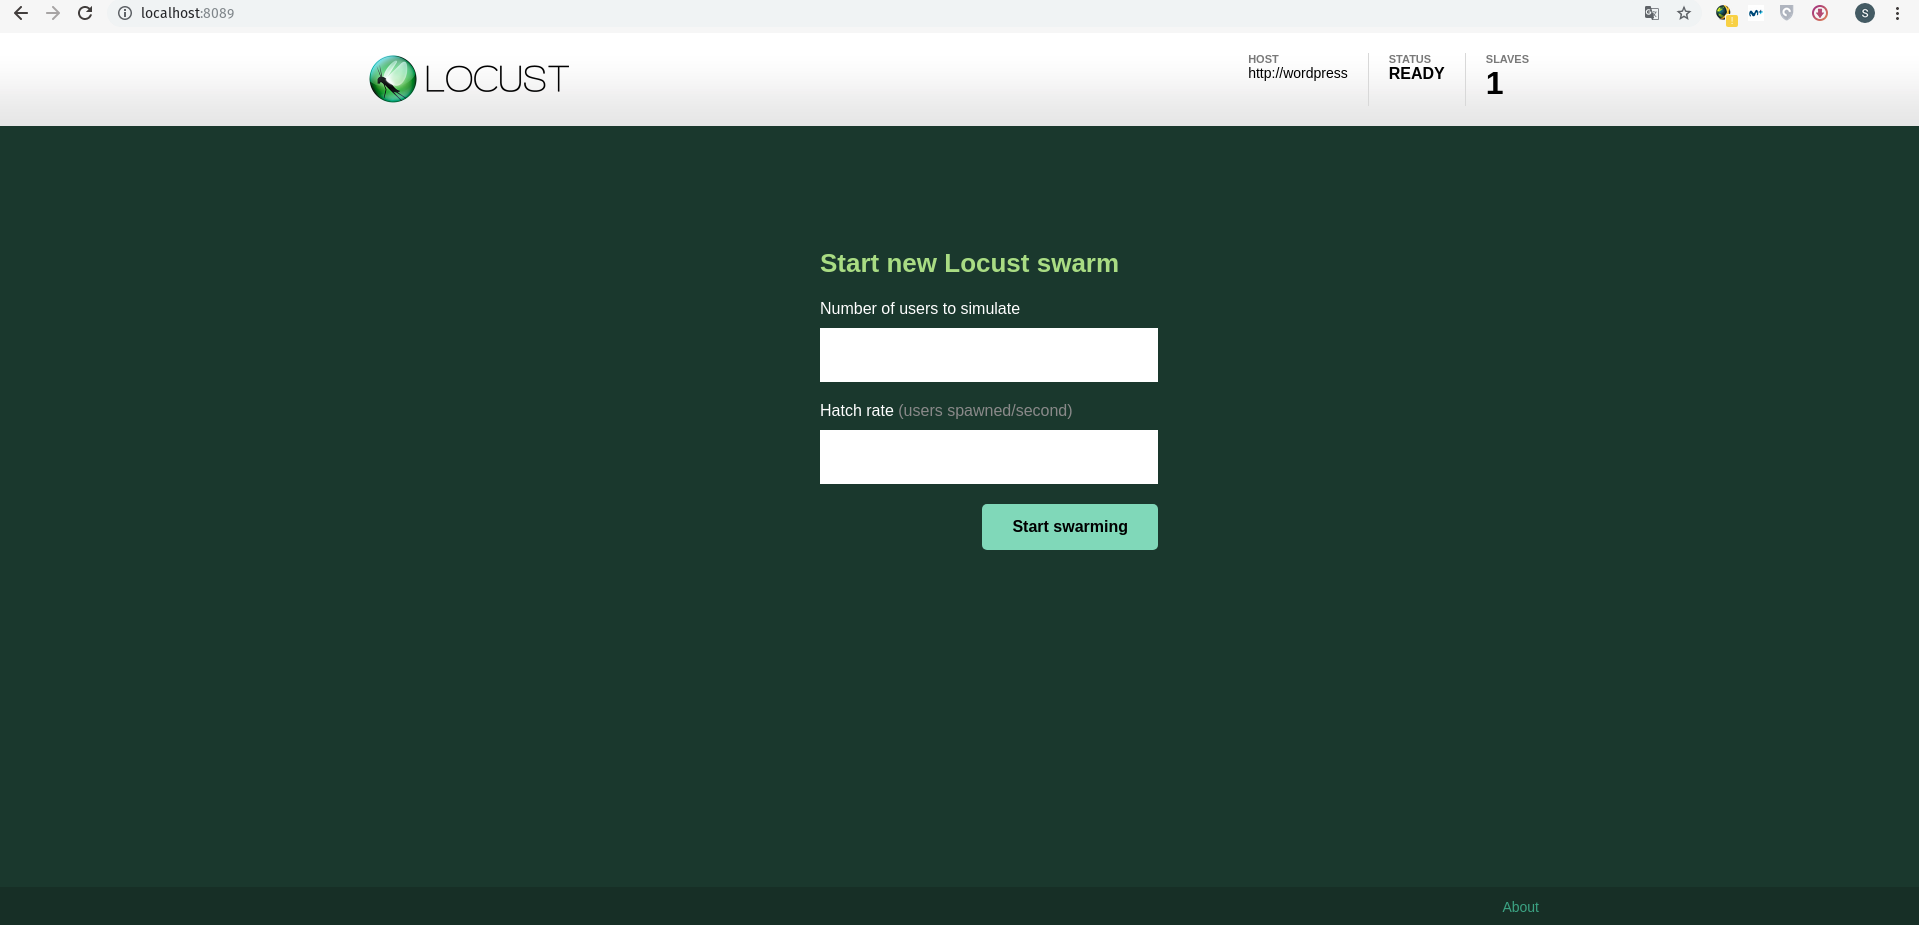
\includegraphics[scale=0.2]{imagenes/carga/locustInterfaz.png}
	\caption{Interfaz Locust} \label{locust_interfaz}
\end{figure}

Si ejecutamos como Number of users con valor 10 y el Hatch rate con valor 1 tenemos que cuando se inicie la prueba de carga con esta configuración, Locust generará 1 nuevo usuario por cada segundo hasta que alcance el número total de usuarios a simular (que en este caso es 10). Cuando alcanza el número de usuarios, la estadística se restablecerá.
\newpage
Esta explicación viene representada de forma gráfica de la siguiente manera:

\begin{figure}[H]
	\centering
	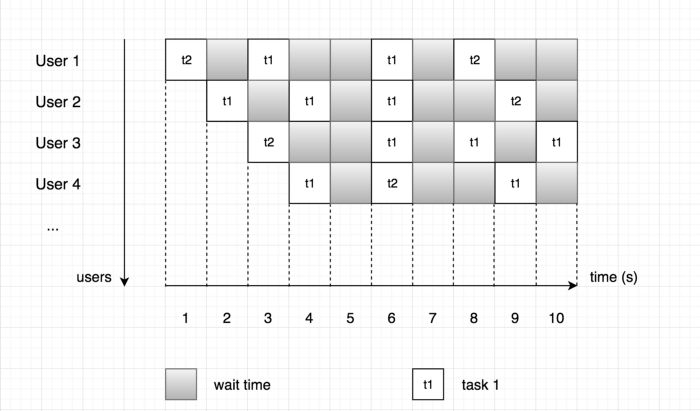
\includegraphics[scale=0.2]{imagenes/carga/explicacion_locust.png}
	\caption{Realización de tareas concurrentes} \label{locust}
\end{figure}

Después de establecer estos valores, se podrá ver el resultado de la prueba en tiempo real:
\begin{figure}[H]
	\centering
	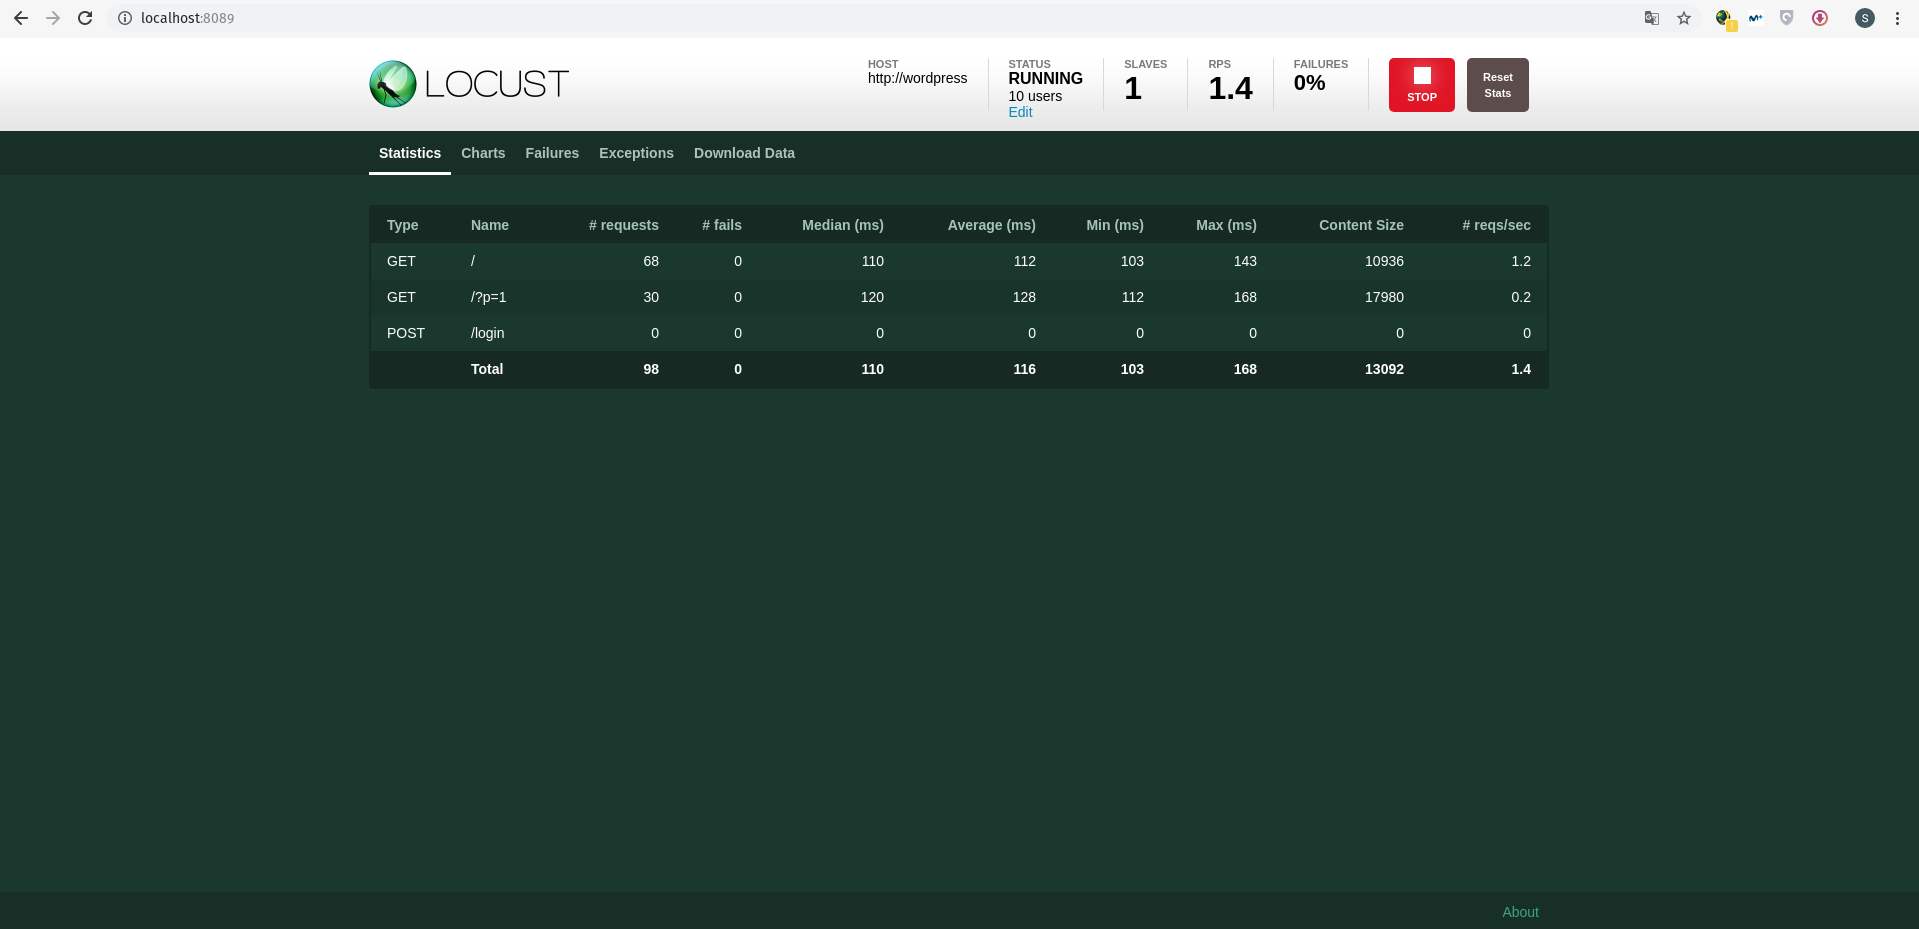
\includegraphics[scale=0.2]{imagenes/carga/pruebalocust.png}
	\caption{Pruebas de tareas concurrentes} \label{locust_prueba}
\end{figure}

Una vez que se ha alcanzado el número deseado de solicitudes, se puede detener la herramienta \textbf{Locust }desde la interfaz web. También permite restablecer las estadísticas o ejecutar una nueva prueba o test.
Además de las estadísticas, puede mirar los \textbf{gráficos} (segunda pestaña) o cualquier \textbf{fallo o excepción que se haya recibido} (tercera, cuarta pestaña), así como \textbf{descargar los resultados de las pruebas como archivos CSV} (la última pestaña).
\newpage
\begin{figure}[H]
	\centering
	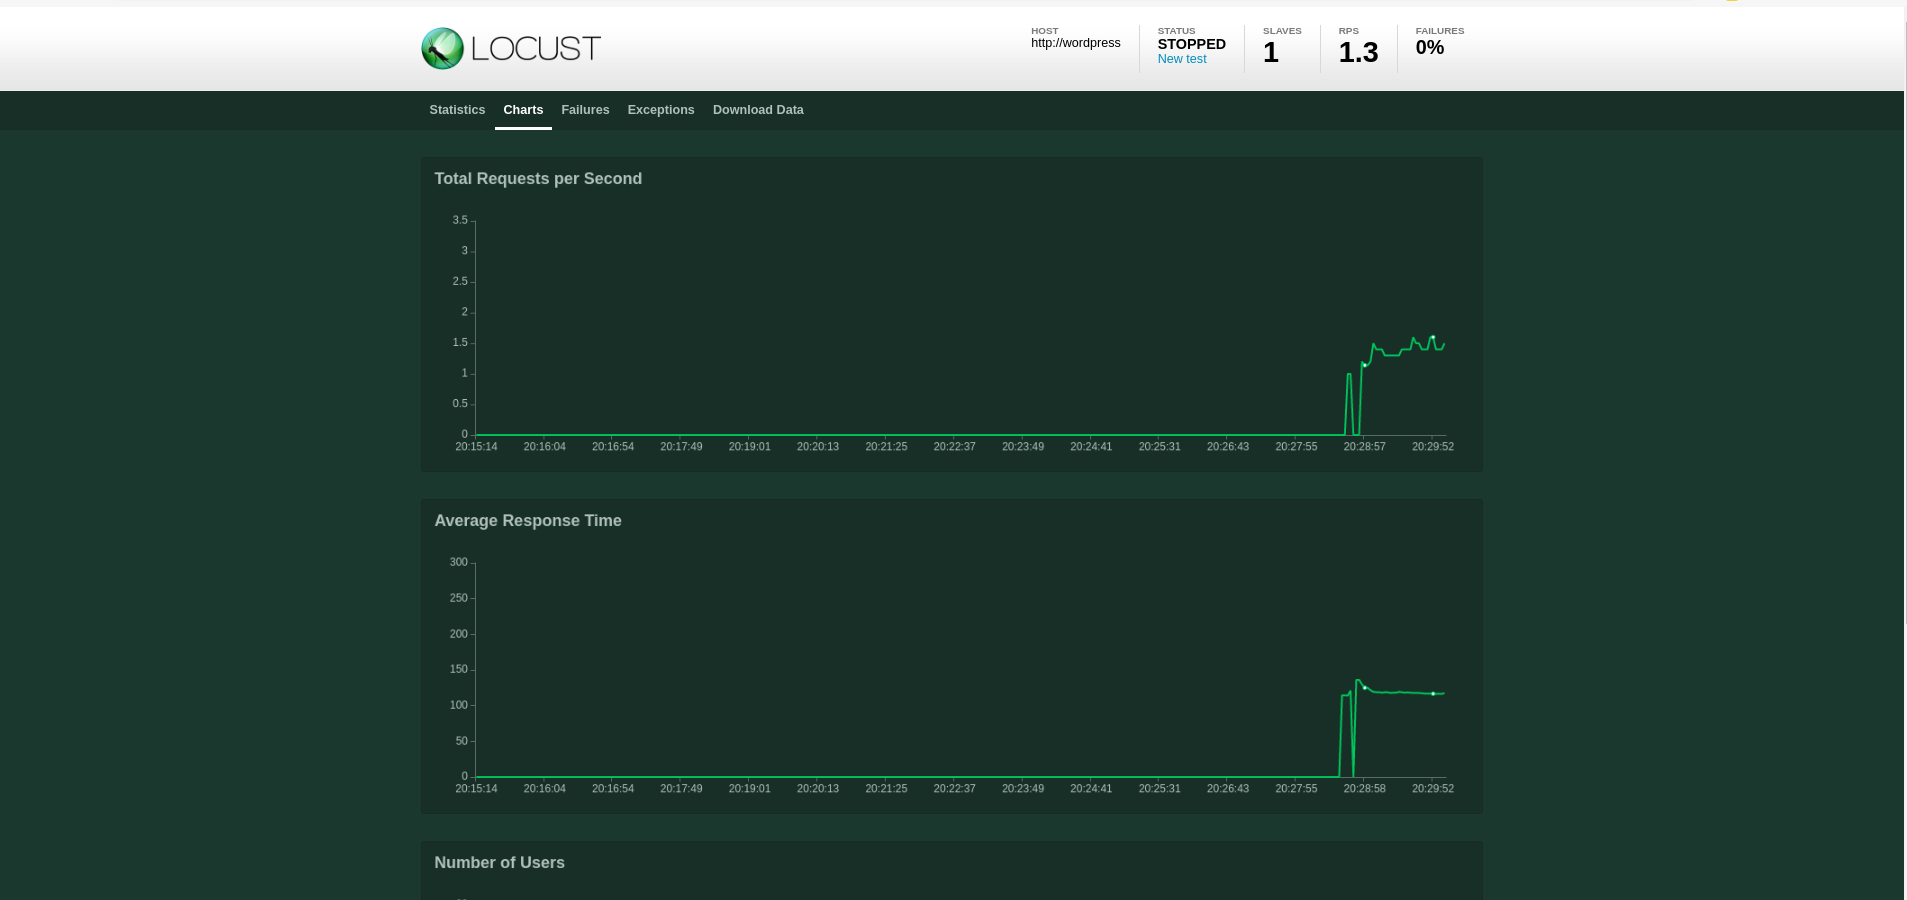
\includegraphics[scale=0.2]{imagenes/carga/charts.png}
	\caption{Gráfico generado en las ejecuciones} \label{locust_chart}
\end{figure}

Básicamente, las\textbf{ solicitudes por segundo}, es decir, el \textbf{rendimiento} indican la cantidad de transacciones por segundo que la aplicación puede realizar.

El \textbf{tiempo de respuesta }es la cantidad de tiempo desde el momento en que un usuario envía una solicitud hasta el momento en que su aplicación indica que la solicitud se ha completado.
 
En el gráfico anterior se puede ver la correlación entre los \textbf{tiempos de respuesta y el rendimiento}. El \textbf{rendimiento} general tiende a disminuir a medida que aumenta el tiempo de respuesta para una transacción promedio. El \textbf{motivo} es que después de enviar la primera solicitud, \textbf{Locust} debe esperar hasta que la solicitud se complete o se procese para enviar la segunda solicitud. 

\section{Pruebas de monitorización en Naemon}
En esta sección vamos a empezar con  la \textbf{puesta en marcha de la herramienta Naemon a través del análisis del sistema realizado}, es decir, el sistema WordPress. Como se señaló en el capítulo \ref{ch:estado}, donde especificabamos la carpeta de configuración de los distintos equipos y servicios a monitorizar, esta es la carpeta \textbf{/etc/naemon/conf.d}, en esta carpeta aplicaremos la configuración correspondiente para analizar el sistema WordPress.
\newpage
Por defecto, Naemon configura la siguiente estructura de archivos y carpetas dentro de la carpeta anterior:
\begin{figure}[H]
	\centering
	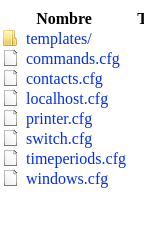
\includegraphics[scale=0.7]{imagenes/wordpress/analisis_naemon/estructura_1.png}
	\caption{Contenido de /etc/naemon/conf.d} \label{conf}
\end{figure}
Dentro de la carpeta \textbf{templates} encontramos el siguiente contenido:
\begin{figure}[H]
	\centering
	
\includegraphics[scale=0.5]{imagenes/wordpress/analisis_naemon/estructura_templates.png}
	\caption{Contenido de /etc/naemon/conf.d/templates} \label{templates}
\end{figure}

Dentro de la carpeta \textbf{templates} podemos encontrar plantillas de ejemplos de hosts y services, donde el contenido de estos lo vamos a aplicar en la creación de nuestros archivos de configuración.
\newpage
El archivo \textbf{localhost.cfg} es una plantilla de ejemplo del analisis de un servidor linux, tomaremos de ejemplo este para realizar las diferentes configuraciones, para poder introducir nuestros nuevos archivos de configuración, debemos modificar la imagen que creamos anteriormente para desplegar Naemon, donde incluiremos las siguientes líneas, donde añadiremos un archivo de incorporación de hosts y de servicios, además de eliminar dicho archivo \textbf{localhost.cfg}:

\begin{lstlisting}[language=bash]
RUN rm -rf /etc/naemon/conf.d/localhost.cfg
ADD definition/wordpresshosts.cfg /etc/naemon/conf.d/wordpresshosts.cfg 
ADD definition/wordpressservices.cfg /etc/naemon/conf.d/wordpressservices.cfg 
\end{lstlisting}

A continuación se muestra el \textbf{contenido} de los dos nuevos archivos:

\begin{figure}[H]
	\centering
	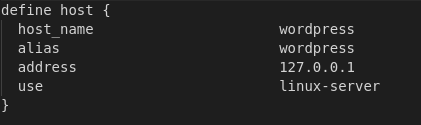
\includegraphics[scale=0.4]{imagenes/wordpress/analisis_naemon/host.png}
	\caption{Contenido del archivo de configuración del host} \label{host}
\end{figure}

\begin{figure}[H]
	\centering
	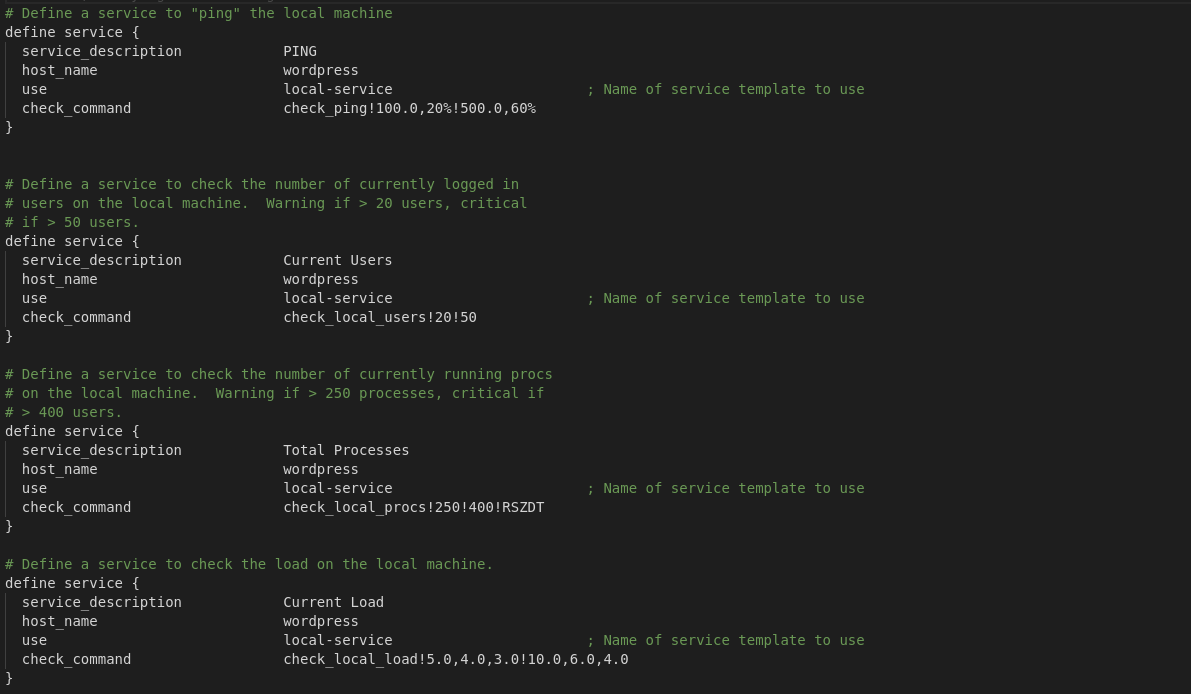
\includegraphics[scale=0.3]{imagenes/wordpress/analisis_naemon/services1.png}
	\caption{Contenido del archivo de configuración del services} \label{services1}
\end{figure}
\newpage
\begin{figure}[H]
	\centering
	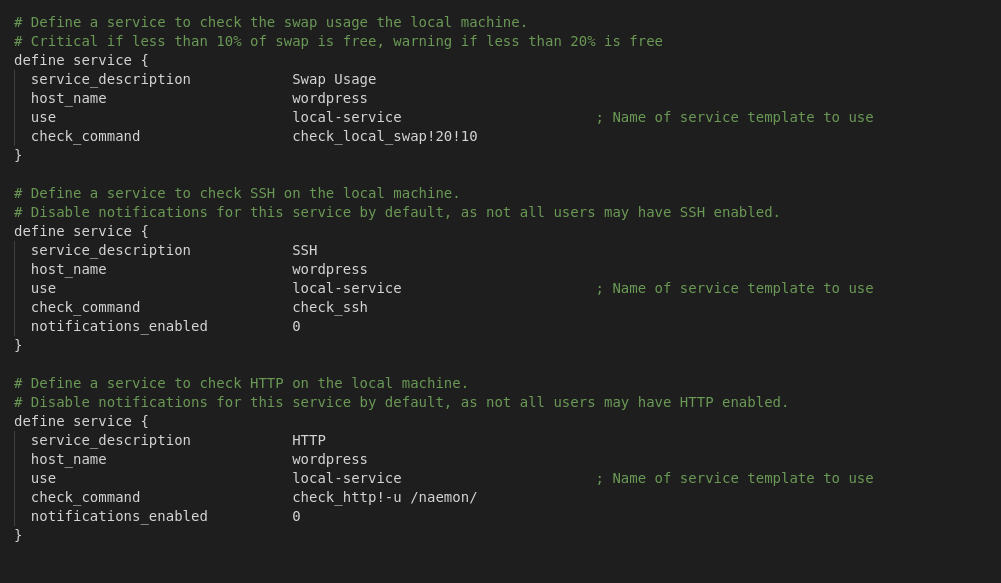
\includegraphics[scale=0.3]{imagenes/wordpress/analisis_naemon/services2.png}
	\caption{Contenido del archivo de configuración del services} \label{services2}
\end{figure}
En los siguientes apartados, se explicará las definiciones que se han realizado.
\subsection{Definición del host}

A través del archivo llamado con el nombre \textbf{wordpresshosts.cfg} se ha realizado la definición del host correspondiente al sistema wordpress, donde a través de:

\begin{itemize}
	\item La etiqueta \textbf{host\_name}, asigna el nombre del host, el cual se ha designado como \textbf{wordpress}.
	\item La etiqueta \textbf{alias},asigna un alias al host, el cual se ha designado como \textbf{wordpress}.
	\item La etiqueta \textbf{address},se encarga de establecer la dirección IP donde se encontrará el host ubicado. Estableceremos \textbf{127.0.0.1 }que será nuestro \textbf{localhost}
	\item La etiqueta \textbf{use}, esta etiqueta se utiliza para usar una plantilla concreta, en este caso usaremos la creada por Naemon, la llamada \textbf{linux-server}, que hablaremos de ella a continuación.
\end{itemize}
\newpage
El host utilizado \textbf{linux-server} se trata de un host creado por Naemon, que no contiene funcionalidad, pero utilizaremos como plantilla para poder trabajar, ya que este se encarga de definir el tiempo por el cual va a estar trabajando el host, además de comprobar en todo momento si está en activo, mediante el plugin \textbf{check-host-alive}. Este host se basa en \textbf{generic-host}, ésta se trata de otra plantilla, a continuación mostramos el contenido de cada plantilla de los host:
 

\begin{lstlisting}[language=bash]

define host {
	name                           generic-host                        ; 
	event_handler_enabled          1                                   ; 
	flap_detection_enabled         1                                   ; 
	notification_period            24x7                                ; 
	notifications_enabled          1                                   ; 
	process_perf_data              1                                   ; 
	register                       1                                   ; 
	retain_nonstatus_information   1                                   ; 
	retain_status_information      1                                   ; 
}


define host {
	name                           linux-server                        ; 
	use                            generic-host                        ; 
	check_command                  check-host-alive                    ; 
	check_interval                 5                                   ; 
	check_period                   24x7                                ; 
	contact_groups                 admins                              ; 
	max_check_attempts             10                                  ; 
	notification_interval          120                                 ; 
	notification_options           d,u,r                               ; 
	notification_period            workhours                           ; 
	register                       1                                   ; 
	retry_interval                 1                                   ; 
}

\end{lstlisting}
\newpage
Las directivas de la definición de los host se explicaron en el capítulo de Estado de Arte \ref{ch:estado}, en este caso el funcionamiento concreto que se ha establecido para el host \textbf{generic-host} es el siguiente:

\begin{itemize}
	\item A través de la directiva \textbf{event\_handler\_enabled} a 1 hemos habilitado el controlador de eventos del host.
	\item A través de la directiva \textbf{flap\_detection\_enabled} a 1 hemos habilitado la detección de flaps del host.
	\item A través de la directiva \textbf{notification\_period} se ha indicado que esté dispuesto 24h a la semana.
	\item A través de la directiva \textbf{notifications\_enabled} a 1 hemos habilitado las notificaciones del host.
	\item A través de la directiva \textbf{process\_perf\_data} a 1 habilita el procesamiento de datos de rendimiento.
	\item A través de la directiva \textbf{register} a 1 hace que se registre el host.
	\item A través de la directiva \textbf{retain\_nonstatus\_information} a 1 habilita la retención de información sin estado.
	\item A través de la directiva \textbf{retain\_status\_information} a 1 habilita la retención de información de estado.
\end{itemize}

El funcionamiento concreto que se ha establecido para el host \textbf{linux-server} es el siguiente:

\begin{itemize}
	\item A través de la directiva \textbf{use} hace que herede la información de generic-host.
	\item A través de la directiva \textbf{check\_command} se intentará hacer un ping al host para ver si está vivo o activado.
	\item A través de la directiva \textbf{check\_interval} se establecerá el valor 5 como unidad de tiempo entre las distintas comprobaciones realizadas.
	\item A través de la directiva \textbf{check\_period} se activará una comprobación de 24h a la semana.
	\item A través de de la directiva \textbf{contact\_groups} se especificará que el grupo al que se notificará es al creado llamado admins.
	\item A través de la directiva \textbf{max\_check\_attempts} con valor 10, indicará que realizará diez veces el intento del comando de verificación del host.
	\newpage
	\item A través de la directiva \textbf{notifications\_enabled} a 1 hemos habilitado las notificaciones del host.
	\item A través de la directiva \textbf{notification\_period} se ha indicado que esté dispuesto en horas laborables.
	\item A través de la directiva \textbf{register} a 1 hace que se registre el host.
	
\end{itemize}

\subsubsection{Host utilizado en la prueba de monitorización del sistema}

En la figura \ref{host} se muestra la configuración del host que se va a utilizar en nuestra prueba, para ello aplicaremos el uso de la plantilla ya creada y explicada \textbf{linux-server}, lo único que tendremos que especificar para la creación de este nuevo host es la \textbf{dirección IP} desde donde se va encontrar el host creado y el nombre del nombre, el cual llamaremos como el sistema utilizado, es decir, \textbf{wordpress}.

Si accedemos a Naemon a través de la GUI de Thruk, podremos ver reflejado la creación de este nuevo host. La información establecida del host vendrá reflejado en la figura \ref{wordpresshost}.
\begin{figure}[H]
	\centering
	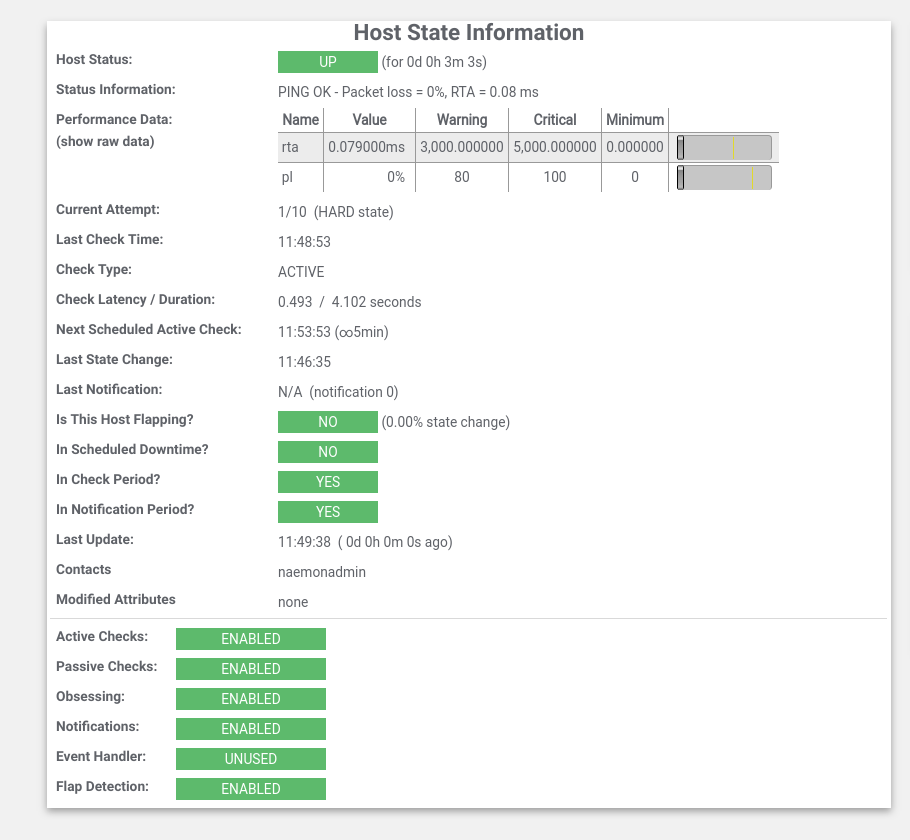
\includegraphics[scale=0.3]{imagenes/wordpress/analisis_naemon/wordpress_host.png}
	\caption{Información del host en Naemon} \label{wordpresshost}
\end{figure}
\newpage
Como podemos observar el host se encuentra activo, ya que su estado es \textbf{UP}, además al indicarle que heredase las directivas de linux-server aparecerán también reflejadas en la información anteriormente mostrada.

En este caso a la hora de ejecutar el \textbf{PING}, servicio que explicaremos en el apartado siguiente, hacia este host, podemos ver que lo realiza de forma correcta, por lo que no se genera pérdida de datos ni paquetes, ya que además en la información mostrada se puede apreciar ese dato. Además mostrará el valor del \textbf{RTA} o lo que es lo mismo \textit{``round trip average"}, que medirá la velocidad de transferencia de los datos, siendo este un valor bastante reducido como se muestra en la figura \ref{wordpresshost}.

\subsection{Definición de los servicios}
A través de este archivo, definiremos los \textbf{servicios} que usaremos en los \textbf{chequeos} o comprobaciones. Se define la métrica o el servicio a monitorizar sobre el que se ejecuta.
Como en el caso del host se ha establecido el uso de la plantilla aportada por Naemon, es decir, se ha utilizado la plantilla \textbf{local-service}.

\begin{lstlisting}[language=bash]

define service {
	name                           generic-service                     ; 
	active_checks_enabled          1                                   ; 
	check_freshness                0                                   ; 
	check_interval                 10                                  ; 
	check_period                   24x7                                ; 
	contact_groups                 admins                              ; 
	event_handler_enabled          1                                   ; 
	flap_detection_enabled         1                                   ; 
	is_volatile                    0                                   ; 
	max_check_attempts             3                                   ; 
	notification_interval          60                                  ; 
	notification_options           w,u,c,r                             ; 
	notification_period            24x7                                ; 
	notifications_enabled          1                                   ; 
	obsess_over_service            1                                   ; 
	passive_checks_enabled         1                                   ; 
	process_perf_data              1                                   ; 
	register                       1                                   ; 
	retain_nonstatus_information   1                                   ; 
	retain_status_information      1                                   ; 
	retry_interval                 2                                   ; 
}


define service {
	name                           local-service                       ; 
	use                            generic-service                     ; 
	check_interval                 5                                   ; 
	max_check_attempts             4                                   ; 
	register                       1                                   ; 
	retry_interval                 1                                   ; 
}

\end{lstlisting}
Las directivas de la definición de los servicios se explicaron en el capítulo de Estado de Arte \ref{ch:estado}, como se ha realizado para la definición del host, a continuación se explicará el funcionamiento a seguir del servicio \textbf{generic-service} y \textbf{local-service}.

Para \textbf{generic-service} las directivas de funcionamiento establecidas son las siguientes:
\begin{itemize}
	
	\item \textbf{is\_volatile}: lo establecemos a 0 para indicar que no será un servicio volátil, es decir, no queremos que se pierda o se elimine la información recogida por el servicio.
	\item \textbf{max\_check\_attempts}:se utiliza para definir la cantidad de veces que Naemon volverá a intentar el comando de verificación de servicio si devuelve cualquier estado que no sea OK. 	Por lo que esto lo realizará una cantidad de tres veces.
	\item \textbf{check\_interval}: se establecerá el valor 10 como unidad de tiempo entre las distintas comprobaciones realizadas.
	\item \textbf{retry\_interval}: se establecerá el valor 2 como unidad de tiempo a esperar antes de programar una nueva verificación del servicio.
	\newpage
	\item \textbf{active\_checks\_enabled}: habilita las comprobaciones activas del servicio.
	\item \textbf{passive\_checks\_enabled}: habilita las comprobaciones pasivas del servicio.
	\item \textbf{check\_period}: se activará una comprobación de 24h a la semana.	
	\item \textbf{obsess\_over\_service|obsess}	: habilita las comprobaciones para el servicio estarán sobrecargadas con el uso del comando ocsp\_command. 
	\item \textbf{check\_freshness}: deshabilita las comprobaciones de actualización ya que esto puede suponer una carga sobre el servicio. 	
	\item \textbf{event\_handler\_enabled}: habilita el controlador de eventos de servicio.
	\item \textbf{flap\_detection\_enabled}: habilita la detección de flaps de servicio.
	\item \textbf{process\_perf\_data}:habilita el procesamiento de datos de rendimiento.
	\item \textbf{retain\_status\_information}: habilitar la retención de información de estado.
	\item \textbf{retain\_nonstatus\_information}: habilitar la retención de información sin estado.
	\item \textbf{notification\_interval}: esperará 60 minutos para volver a notificar a un contacto que este servicio todavía está en un estado no correcto.	

	\item \textbf{notification\_period}: se ha indicado que esté dispuesto 24h a la semana.
	\item \textbf{notification\_options}: se enviarán notificaciones en caso de estado de ADVERTENCIA, DESCONOCIDO, CRÍTICO Y RECUPERACIÓN. 
	\item \textbf{notifications\_enabled}: habilitar notificaciones de servicio. 
	\item \textbf{contact\_groups}: notificará a los grupos administrados, identificados como \textbf{admins}.
	
\end{itemize}
\newpage
Para \textbf{local-service} las directivas de funcionamiento establecidas son las siguientes:
\begin{itemize}	
	\item \textbf{use}: indicará que heredará las directivas de generic-service.
	\item \textbf{max\_check\_attempts}:se utiliza para definir la cantidad de veces que Naemon volverá a intentar el comando de verificación de servicio si devuelve cualquier estado que no sea OK. 	Por lo que esto lo realizará una cantidad de cinco veces.
	\item \textbf{check\_interval}: se establecerá el valor 4 como unidad de tiempo entre las distintas comprobaciones realizadas.
	\item \textbf{retry\_interval}: se establecerá el valor 1 como unidad de tiempo a esperar antes de programar una nueva verificación del servicio.
	\item A través de la directiva \textbf{register} a 1 hace que se registre el servicio.

\end{itemize}
\subsubsection{Servicios utilizados en la prueba de monitorización del sistema}

En las figuras \ref{services1} y \ref{services2} se muestran la configuración de los servicios que se van a utilizar en nuestra prueba, para ello aplicaremos el uso de la plantilla ya creada y explicada \textbf{local-service y generic-service}.

Si accedemos a \textbf{Naemon} a través de la \textbf{GUI de Thruk}, podremos ver reflejada la creación de estos servicios. La información establecida del host con cada servicio vinculado vendrá reflejado en la figura \ref{wordpressservices}.
\begin{figure}[H]
	\centering
	
	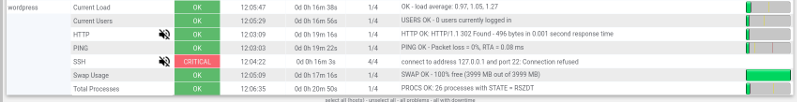
\includegraphics[scale=0.4]{imagenes/wordpress/analisis_naemon/wordpress_services.png}
	\caption{Información del host con cada servicio vinculado en Naemon} \label{wordpressservices}
\end{figure}
A continuación vamos a hablar en detalle de cada servicio definido en el archivo \textbf{wordpressservices.cfg}. 
\newpage
\paragraph{Servicio PING}

A través de la directiva check\_command haremos uso del plugin \textbf{check\_ping}, por el cual hacemos uso de la llamada PING para comprobar las estadísticas de conexión del host.

Para este plugin se establecerá el \textbf{umbral $<$rta$>$,$<$pl$>$} donde \textbf{$<$rta$>$} será el tiempo o la velocidad de transferencia media en "ms" que activará un estado de \textbf{WARNING(advertencia) o CRITICAL(crítico)}, además \textbf{$<$pl$>$} es el porcentaje de pérdida de paquetes para activar un estado de alarma.

El uso de este comando suele ser de la siguiente forma:
\begin{lstlisting}
check_ping -H <host_address> -w <wrta>,<wpl>% -c <crta>,<cpl>%
[-p packets] [-t timeout] [-4|-6]

\end{lstlisting}

La función de check\_command aplicará dicho comando plugin con la siguiente forma de definición:
\begin{lstlisting}
check_ping!100.0,20%!500.0,60%
\end{lstlisting} 

Donde se asume que:
\begin{itemize}
	\item Para el estado \textbf{WARNING}: $<$wrta$>$ es 100.0 y $<$wpl$>$ es 0,20.
	\item Para el estado \textbf{CRITICAL}: $<$crta$>$ es 500.0 y $<$cpl$>$ es 0,60
\end{itemize}

Si este comando se accediera a través de una terminal o línea de comandos de forma expandida, se escribiría de la siguiente forma:

\begin{lstlisting}
/usr/lib/naemon/plugins/check_ping -H 127.0.0.1 -w 100.0,20% -c 500.0,60% -p 5
\end{lstlisting}

Donde se establece el host y el número de paquetes a enviar que si no se asume nada se toma por defecto el valor 5.

Este plugin utiliza el comando \textbf{ping} para que el host especificado busque la pérdida de paquetes según un porcentaje y el promedio de ida y vuelta en milisegundos.
\newpage
Si accedemos a la \textbf{GUI de Thruk} podemos observar el registro de información del rendimiento, obteniéndose los siguientes valores:
 
\begin{lstlisting}
rta=0.087000ms;100.000000;500.000000;0.000000 pl=0%;20;60;0
\end{lstlisting}

Por lo que el estado que obtendremos será \textbf{OK}, ya que no se ha perdido ningún paquete y los valores del \textbf{RTA} son tan pequeños que no se encuentran en el estado de \textbf{WARNING ni CRITICAL}.

\paragraph{Servicio para comprobar usuarios actuales registrados}

A través de la directiva \textbf{check\_command} haremos uso del siguiente plugin \textbf{check\_local\_users}, con este plugin comprobaremos el número de usuarios que se encuentran registrados en el servidor o host y genera un error si el número excede los umbrales especificados.

Para este plugin se establecerá el \textbf{umbral para warning y critical}.

El uso de este comando suele ser de la siguiente forma:
\begin{lstlisting}
check_local_users -w <users> -c <users>
\end{lstlisting}

La función de check\_command aplicará dicho comando plugin con la siguiente forma de definición:
\begin{lstlisting}
check_local_users!20!50
\end{lstlisting} 

Donde se asume que:
\begin{itemize}
	\item Para el estado \textbf{WARNING}: se ha establecido un límite de 20 usuarios.
	\item Para el estado \textbf{CRITICAL}: se ha establecido un límite de 50 usuarios.
\end{itemize}

Si este comando se accediera a través de una terminal o línea de comandos de forma expandida, se escribiría de la siguiente forma:

\begin{lstlisting}
/usr/lib/naemon/plugins/check_users -w 20 -c 50
\end{lstlisting}
\newpage
Si accedemos a la \textbf{GUI de Thruk} podemos observar el registro de información del rendimiento, obteniéndose los siguientes valores:

\begin{lstlisting}
USERS OK - 0 users currently logged in

users=0;20;50;0
\end{lstlisting}

Por lo que el estado que obtendremos será \textbf{OK}, ya que no se ha excedido los valores asignados en cuanto a usuarios conectados.
\paragraph{Servicio para comprobar total de procesos ejecutados}

A través de la directiva \textbf{check\_command} haremos uso del siguiente plugin \textbf{check\_local\_procs}, con este plugin comprobaremos todos los procesos y generaremos estados de ADVERTENCIA o CRÍTICOS si la métrica especificada está fuera de los rangos de umbral requeridos. El valor predeterminado de la métrica es el número de procesos. Los filtros de búsqueda se pueden aplicar para limitar los procesos a verificar.

El uso de este comando suele ser de la siguiente forma:
\begin{lstlisting}
check_local_procs -w <range> -c <range> [-m metric] [-s state] [-p ppid]
[-u user] [-r rss] [-z vsz] [-P %cpu] [-a argument-array]
[-C command] [-k] [-t timeout] [-v]
\end{lstlisting}

La función de \textbf{check\_command} aplicará dicho comando plugin con la siguiente forma de definición:
\begin{lstlisting}
check_local_procs!250!400!RSZDT
\end{lstlisting} 

Donde se asume que:
\begin{itemize}
	\item Para el estado \textbf{WARNING}: se ha establecido un límite de 250 procesos.
	\item Para el estado \textbf{CRITICAL}: se ha establecido un límite de 400 procesos.
	\item Se ha establecido el estado \textbf{RSZDT}, el cual significa lo siguiente: \textbf{R:ejecutable,S:esperando de forma dormida,Z:proceso zombie que termina pero no se repite por su padre, D: ininterrumpible, T:parado por una señal de control}.
\end{itemize}
\newpage
Si este comando se accediera a través de una terminal o línea de comandos de forma expandida, se escribiría de la siguiente forma:

\begin{lstlisting}
/usr/lib/naemon/plugins/check_procs -w 250 -c 400 -s RSZDT
\end{lstlisting}

Si accedemos a la \textbf{GUI de Thruk} podemos observar el registro de información del rendimiento, obteniéndose los siguientes valores:

\begin{lstlisting}
PROCS OK: 26 processes with STATE = RSZDT

procs=26;250;400;0;
\end{lstlisting}

Por lo que el estado que obtendremos será \textbf{OK}, ya que no se ha excedido los valores asignados en cuanto a procesos creados.
\paragraph{Servicio para comprobar la carga actual}

A través de la directiva check\_command haremos uso del plugin \textbf{check\_local\_load}, con este plugin comprobaremos el promedio de carga actual del sistema.

El uso de este comando suele ser de la siguiente forma:
\begin{lstlisting}
check_local_load [-r] -w WLOAD1,WLOAD5,WLOAD15 -c CLOAD1,CLOAD5,CLOAD15 [-n NUMBER_OF_PROCS]
\end{lstlisting}

\begin{itemize}
	\item Donde\textbf{ -r }se encarga de dividir el porcentaje de carga por el número de CPUs, pero esto solo cuando sea posible.
	\item Notificará con el estado de \textbf{ADVERTENCIA} si el promedio de carga excede el valor asignado en WLOADn
	\item Notificará con el estado de \textbf{CRÍTICO} si el promedio de carga excede el valor asignado en CLOADn
\end{itemize}


La función de \textbf{check\_command} aplicará dicho comando plugin con la siguiente forma de definición:
\begin{lstlisting}	
check_local_load!5.0,4.0,3.0!10.0,6.0,4.0
\end{lstlisting} 
\newpage
Donde se asume que:
\begin{itemize}
	\item Para el estado \textbf{WARNING}: se ha establecido las cargas de 5.0, 4.0 y 3.0
	\item Para el estado \textbf{CRITICAL}: se ha establecido las cargas de 10.0, 6.0 y 4.0	
\end{itemize}

Si este comando se accediera a través de una terminal o línea de comandos de forma expandida, se escribiría de la siguiente forma:

\begin{lstlisting}
/usr/lib/naemon/plugins/check_load -w 5.0,4.0,3.0 -c 10.0,6.0,4.0
\end{lstlisting}

Si accedemos a la \textbf{GUI de Thruk} podemos observar el registro de información del rendimiento, obteniéndose los siguientes valores:

\begin{lstlisting}
OK - load average: 0.35, 0.64, 0.68

load1=0.350;5.000;10.000;0; load5=0.640;4.000;6.000;0; load15=0.680;3.000;4.000;0;
\end{lstlisting}

Por lo que el estado que obtendremos será \textbf{OK}, ya que no se ha excedido los valores asignados en cuanto a carga ejecutada.
\paragraph{Servicio para comprobar el uso de intercambio}

A través de la directiva check\_command haremos uso del plugin \textbf{check\_local\_swap}, con este plugin comprobaremos el espacio de intercambio en la máquina local.

El uso de este comando suele ser de la siguiente forma:
\begin{lstlisting}
check_swap [-av] -w <percent_free>% -c <percent_free>%
-w <bytes_free> -c <bytes_free> [-n <state>]
\end{lstlisting}

\begin{itemize}
	\item Notificará con el estado de \textbf{ADVERTENCIA} si hay menos del porcentaje de espacio de intercambio libre o si hay menos bytes de espacio de intercambio libres.
	\item Notificará con el estado de \textbf{CRÍTICO}  si hay menos del porcentaje de espacio de intercambio libre o si hay menos bytes de espacio de intercambio libres.
\end{itemize}


La función de \textbf{check\_command} aplicará dicho comando plugin con la siguiente forma de definición:
\begin{lstlisting}	
check_local_swap!20!10

\end{lstlisting} 

Donde se asume que:
\begin{itemize}
	\item Para el estado \textbf{WARNING}: se ha establecido a 20 el límite
	\item Para el estado \textbf{CRITICAL}: se ha establecido a 10 el límite
\end{itemize}

Si este comando se accediera a través de una terminal o línea de comandos de forma expandida, se escribiría de la siguiente forma:

\begin{lstlisting}
/usr/lib/naemon/plugins/check_swap -w 20 -c 10
\end{lstlisting}

Si accedemos a la \textbf{GUI de Thruk} podemos observar el registro de información del rendimiento, obteniéndose los siguientes valores:

\begin{lstlisting}
SWAP OK - 100% free (3999 MB out of 3999 MB)

swap=3999MB;0;0;0;3999

\end{lstlisting}

Por lo que el estado que obtendremos será \textbf{OK}, ya que no se ha excedido los valores asignados, esto es debido a que nos encontramos en una máquina local sin tener a cargo una máquina Windows o Linux activada en el host.

\paragraph{Servicio para comprobar el protocolo SSH}

A través de la directiva check\_command haremos uso del plugin \textbf{check\_SSH}, con este plugin comprobaremos \textbf{el protocolo SSH}. Intentará conectarse a un servidor SSH en el servidor y puerto especificados

El uso de este comando suele ser de la siguiente forma:
\begin{lstlisting}
check_ssh  [-4|-6] [-t <timeout>] [-r <remote version>] [-p <port>] <host>
\end{lstlisting}
\newpage
\begin{itemize}
	\item Donde\textbf{ -t } define los segundos antes del tiempo de espera de la conexión por defecto es 10.
	\item Donde\textbf{ -r } alerta si la cadena no coincide con la versión esperada del servidor.
	\item Donde\textbf{ -p } define el puerto a especificar.
	\item Se debe establecer el host por el cual se comprobará la conexión SSH.
\end{itemize}

La función de \textbf{check\_command} aplicará dicho comando plugin con la siguiente forma de definición:
\begin{lstlisting}	
check_ssh
\end{lstlisting} 

Si este comando se accediera a través de una terminal o línea de comandos de forma expandida, se escribiría de la siguiente forma:

\begin{lstlisting}
/usr/lib/naemon/plugins/check_ssh  127.0.0.1
\end{lstlisting}

Si accedemos a la \textbf{GUI de Thruk} podemos observar el registro de información del rendimiento, obteniéndose los siguientes valores:

\begin{lstlisting}
connect to address 127.0.0.1 and port 22: Connection refused
\end{lstlisting}

Esto es debido a que no se dió acceso al puerto 22 a la hora de realizar la creación del \textbf{Dockerfile}.
Esto queda arreglado haciendo una llamada a \textbf{EXPOSE 22} en el archivo \textbf{Dockerfile}.
\newpage
Y además añadiendo un nuevo servicio en \textbf{docker-compose.yml} llamado como el propio protocolo \textbf{ssh}. Esto quedará reflejado de la siguiente forma en dicho archivo:
\begin{lstlisting}
	ssh:
	image: "jdeathe/centos-ssh:2.2.1"
	volumes:
	- "wp_html:/var/www/html"
	- "wp_ssh_keys:/etc/ssh"
	ports:
	- "80:22"
	environment:
	SSH_USER: "wordpress"
	SSH_USER_ID: "65534:65534"
	SSH_USER_HOME: "/var/www"
	SSH_USER_PASSWORD_HASHED: "true"
	SSH_USER_PASSWORD: "wordpress"
	SSH_AUTHORIZED_KEYS: "ssh-rsa AAAAB3NzaC1yc2EAAAADAQABAAABAQC9wfq9fZfn9JicyTq//
	peCAd9gQ7mi4vCIoBzx0zGXmSWsY+4TijbDK2Xb9ZuQw8tyCg9rjZ24W2mvfM6+tpC7nVZRvvsSOji641hN9FamBt34+
	oTeOMXyE1WH5dGDdwLHYYXAo/R/
	yNBlxzT1QaqRjA9PJgcrrV2LsnT/6rbrX1x3mOG0M1KytOTHiHhUlNfRCnGFR
	6Velkx8RNj9z8zI9kqaJTICew1Ss1WFDo+02Ij26Xp4JdK4qCCRGSyv6QTbNekN7
	icp25dYK1XsxTiT+N7CYvgOEEeb/lRRzYX9c0JWbaqhiASLo1cYwkWCONqewjID4OQkYjN9JrqdOnb/"
	restart: "always"
\end{lstlisting}
Con esto tendríamos la conexión SSH asegurada, recibiendo el estado \textbf{OK} en la GUI de Naemon. 
\paragraph{Servicio para comprobar el protocolo HTTP}

A través de la directiva check\_command haremos uso del plugin \textbf{check\_http}, con este plugin comprobaremos el servicio HTTP en el host especificado. Se puede probar
servidores normales (\textbf{http}) y seguros (\textbf{https}).
El uso de este comando suele ser de la siguiente forma:
\begin{lstlisting}
check_http -H <vhost> | -I <IP-address> [-u <uri>] [-p <port>]
[-J <client certificate file>] [-K <private key>]
[-w <warn time>] [-c <critical time>] [-t <timeout>] [-L] [-E] [-a auth]
[-b proxy_auth] [-f <ok|warning|critcal|follow|sticky|stickyport>]
[-e <expect>] [-d string] [-s string] [-l] [-r <regex> | -R <case-insensitive regex>]
[-P string] [-m <min_pg_size>:<max_pg_size>] [-4|-6] [-N] [-M <age>]
[-A string] [-k string] [-S <version>] [--sni] [-C <warn_age>[,<crit_age>]]
[-T <content-type>] [-j method]
\end{lstlisting}
\newpage
La función de \textbf{check\_command} aplicará dicho comando plugin con la siguiente forma de definición:
\begin{lstlisting}	
check_http!-u /naemon/
\end{lstlisting} 

Donde se asume que:
\begin{itemize}
	\item La ruta asignada lo realizará a través de -u asignando la ruta /naemon/
\end{itemize}

Si este comando se accediera a través de una terminal o línea de comandos de forma expandida, se escribiría de la siguiente forma:

\begin{lstlisting}
/usr/lib/naemon/plugins/check_http -I 127.0.0.1 -u /naemon/
\end{lstlisting}

Si accedemos a la \textbf{GUI de Thruk} podemos observar el registro de información del rendimiento, obteniéndose los siguientes valores:

\begin{lstlisting}
HTTP OK: HTTP/1.1 302 Found - 502 bytes in 0.001 second response time

time=0.000893s;;;0.000000;10.000000 size=502B;;;0

\end{lstlisting}

Por lo que el estado que obtendremos será \textbf{OK}, especificando que se ha encontrado el protocolo y el tiempo de respuesta es considerable para su acceso, es decir, realiza una petición GET o POST a dicha ruta asignada.

\section{Puesta en práctica: creación de complemento o plugin}

A continuación para empezar a realizar pruebas crearemos un plugin capaz de comprobar si existe una página concreta, esto es en el caso de que el archivo \textbf{wp-config.php} no se detecte, ya que si no se realiza esta comprobación puede ser que tengamos cuando se realiza el servicio HTTP un OK, cuando este no es el verdadero resultado. Así además se comprueba que la base de datos funciona correctamente. Para comprobar que accede de forma correcta a la base de datos y recoge de forma correcta la información haremos uso del plugin \textbf{check\_http}, aunque realizaremos una modificación, por lo que crearemos un nuevo comando, llamado \textbf{check\_wp\_dominio} y le especificaremos que acceda a la ruta \textbf{/2019/08/16/hola-mundo/}, esta se trata de un artículo concreto de nuestro sistema WordPress.
\newpage
Después para poder hacer uso y mostrar el resultado, definiremos el servicio, donde sólo llamaremos al comando creado heredando como en los anteriores servicios el servicio \textbf{local-service}.

\begin{lstlisting}[language=bash]
define command{
	command_name    check_wp_dominio
	command_line    $USER1$/check_http -H $HOSTADDRESS$ -u /2019/08/16/hola-mundo/
}
define service {
	service_description            WordPress Hola Mundo
	host_name                      wordpress
	use                            local-service                       
	check_command                  check_wp_dominio
}
\end{lstlisting}
En la figura \ref{check_hola_mundo} se muestra el resultado obtenido por el servicio ejecutado anteriormente definido.
\begin{figure}[H]
	\centering
	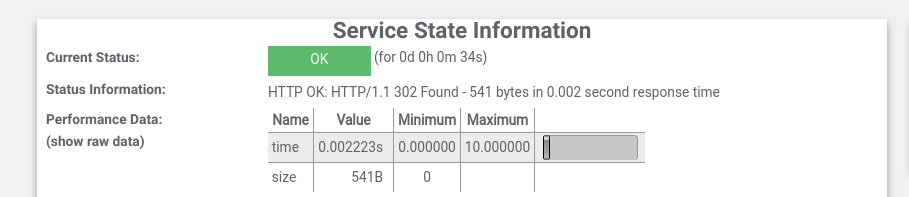
\includegraphics[scale=0.3]{imagenes/wordpress/analisis_naemon/check_hola_mundo.png}
	\caption{Información del estado del plugin de comprobación del puerto 80 sobre la página del artículo Hola, mundo de WordPress} \label{check_hola_mundo}
\end{figure}

Ahora para dar funcionamiento a nuestro sistema y además aplicar la creación de un nuevo plugin o complemento, crearemos uno por el cual compruebe que la ruta indicada por nuestro servicio no se encuentre infectada, es decir, al encontrarnos ante un sistema CMS como WordPress estamos expuestos a gran cantidad de vulnerabilidades externas, por lo que nos apoyaremos de Naemon para monitorizar este estado, para ello crearemos el plugin con nombre \textbf{check\_hackedfiles}.
\newpage
El contenido de este plugin es el siguiente:

\begin{lstlisting}

#!/bin/bash
#

# Config regular expression
REG_EXPR[1]="[0-9a-zA-Z][0-9a-zA-Z][0-9a-zA-Z][0-9a-zA-Z][0-9a-zA-Z][0-9a-zA-Z][0-9a-zA-Z][0-9a-zA-Z][0-9a-zA-Z][0-9a-zA-Z][0-9a-zA-Z][0-9a-zA-Z][0-9a-zA-Z][0-9a-zA-Z][0-9a-zA-Z][0-9a-zA-Z][0-9a-zA-Z][0-9a-zA-Z][0-9a-zA-Z][0-9a-zA-Z]['\"]\.$"
REG_EXPR[2]="[\]x[0-9a-zA-Z][0-9a-zA-Z][\]x[0-9a-zA-Z][0-9a-zA-Z][\]x[0-9a-zA-Z][0-9a-zA-Z][\]x[0-9a-zA-Z][0-9a-zA-Z]"
REG_EXPR[3]="[\]x[0-9a-zA-Z][0-9a-zA-Z][0-9a-zA-Z][\]x[0-9a-zA-Z][0-9a-zA-Z][0-9a-zA-Z]"
REG_EXPR[4]="[\]x[0-9a-zA-Z][0-9a-zA-Z][0-9a-zA-Z][0-9a-zA-Z]"
REG_EXPR[5]="_[0O][0O][0O][0O][0O]"

# EO Config regular expression

# Collection of regular expressions
REG_EXPR=$(printf '%s|' "${REG_EXPR[@]}" | sed 's/|$//')

STATE_OK=0
STATE_WARNING=1
STATE_CRITICAL=2
STATE_UNKNOWN=3

USAGE="Uso: `basename $0` [-h] [-d DIR] [-b NUM] [-l LOG] [-s w/c] [-x FILE]\n
-d [DIR] Directory to check.\n
-b [NUM] Days back.\n
-l [FILE] Log file.\n
-s [w]arning or [c]ritical: Select state when hacked files are present. Default: w\n
-x [FILE] Exclude. List of files to skip check.\n
-e [EXTENSIONS] Exclude file extensions. e.g. \"*.jpg|*.png\"\n
Please use full paths!
"

if [ "$1" == "-h" ] || [ "$1" == "" ] ; then
echo -e $USAGE
exit $STATE_UNKNOWN
fi

while getopts d:b:l:s:x:e: option
do
case "${option}"
in
d) CHECK_DIR=${OPTARG};;
b) DAYS_BACK=${OPTARG};;
l) LOG_FILE=${OPTARG};;
s) RETURN_STATE=${OPTARG};;
x) EXCLUDE_FILES=${OPTARG};;
e) EXCLUDE_FILE_EXTENSIONS=${OPTARG};;
esac
done

### Exit State
if [ -z $RETURN_STATE ]; then
STATE=$STATE_WARNING
else
if [ $RETURN_STATE == "w" ]; then
STATE=$STATE_WARNING
elif [ $RETURN_STATE == "c" ]; then
STATE=$STATE_CRITICAL
else
echo "Bad value for -s!"
echo -e $USAGE
exit $STATE_UNKNOWN
fi
fi
### EO Exit State

### Excludes
if [ -z $EXCLUDE_FILES ]; then
EXCLUDE_PART=""
else
if [ -s "$EXCLUDE_FILES" ]; then 
EXCLUDE_PART=$(printf "! -samefile %s " $(cat $EXCLUDE_FILES))
else
EXCLUDE_PART=""
fi
fi
### EO Excludes

### Exclude file extensions
if [ -z $EXCLUDE_FILE_EXTENSIONS ]; then
EXCLUDE_EXTENSIONS_PART=""
else
EXCLUDE_EXTENSIONS_PART=$(printf "! -name %s " $(echo $EXCLUDE_FILE_EXTENSIONS | sed 's/|/ /g'))
fi
### EO Exclude file extensions

DATE=$(date)

CHECK=$(find $CHECK_DIR -type f \( -name "*" $EXCLUDE_EXTENSIONS_PART $EXCLUDE_PART \) -ctime -$DAYS_BACK -exec grep -lrE "$REG_EXPR" {} \;)

echo "----" >> $LOG_FILE
echo $DATE >> $LOG_FILE

printf '%s\n' "${CHECK[@]}" >> $LOG_FILE


if [ -z "$CHECK" ]; then
echo "OK - There are no infected files for the last $DAYS_BACK days."
exit $STATE_OK
else
echo "There may be infected files from the last $DAYS_BACK days."
exit $STATE
fi

\end{lstlisting}
\newpage
Su \textbf{funcionamiento} es el siguiente:

\begin{itemize}
	\item Dependiendo el valor o la opción a comprobar que se le pase que se le pase, ya sea un directorio, un archivo log, un archivo excluido o un archivo de extensión, parseará con \textbf{getopts} esa opción y la guardará en su correspondiente opción.
	\item Si se ha encontrado con un algún estado \textbf{WARNING O CRITICAL} se encargará de devolver dicho estado.
	\item Empieza la comprobación de cada elementos comprobando que se encuentra dentro del sistema.
	\item En el caso de encontrarse y además contener expresiones regulares que no se encuentran acorde al contenido que deben tener, esta lanzará la opción de que se encuentran infectados y lanzará un \textbf{WARNING o CRITICAL}.
\end{itemize}

Para poder poner este plugin en marcha, es necesario crear el comando correspondiente y su servicio.

\begin{lstlisting}

define command{
	command_name    check_hackedfiles
	command_line    $USER1$/check_hackedfiles $ARG1$
}

define service{
	use                     generic-service,service-pnp    
	host_name               wordpress
	service_description     Hackedfiles
	check_command           check_hackedfiles! /
}

\end{lstlisting}

Este contenido lo ingresaremos en \textbf{wordpresshosts.cfg} y \textbf{wordpressservices.cfg} anteriormente creados y además debemos crear dentro de nuestro \textbf{Dockerfile} la siguiente línea para poder añadir a la carpeta de plugin nuestro archivo nuevo, y le daremos permiso de ejecución:

\begin{lstlisting}
ADD plugins/check_hackedfiles /usr/lib/naemon/plugins/check_hackedfiles
RUN sync && chmod 755 /usr/lib/naemon/plugins/check_hackedfiles
\end{lstlisting}
\newpage
Si lanzamos nuestra ejecución y accedemos a nuestro servicio creado en \textbf{Thruk} podemos visualizar lo reflejado en la figura \ref{check_hackfiles}.

\begin{figure}[H]
	\centering
	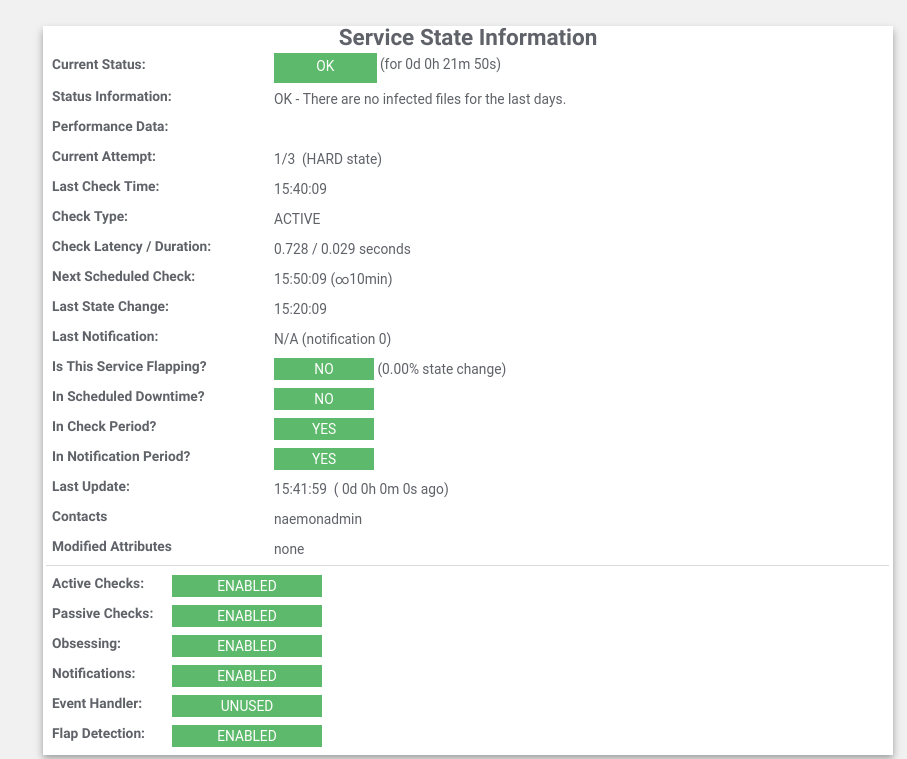
\includegraphics[scale=0.3]{imagenes/wordpress/analisis_naemon/check_hackfiles.png}
	\caption{Información del estado del plugin de comprobación de archivos} \label{check_hackfiles}
\end{figure}

En el capítulo siguiente pasamos a realizar el \textbf{modelado de cargas} de todos los servicios creados en \textbf{Naemon}, es decir, representaremos la carga de trabajo mediante el análisis de prestaciones y crear con esto un modelo.
\newpage
\chapter{Modelado} \label{ch:introduction}

\section{Introducción a la carga de trabajo}
\cite{modelado}
A la hora de realizar un análisis de prestaciones siempre se tiene que tener en cuenta el comportamiento que va a tener un sistema o varios ante una carga concreta de trabajo.

Lo normal es que no se disponga en tiempo real de esta carga a la que se va someter el sistema, pero sí se puede utilizar o aplicar un modelo con características similares o parecidas. Por lo que estos análisis se suelen basar en \textbf{modelos de carga}, es decir, modelos que se extraen tras la caracterización previa de la propia carga. Cuando el modelo se encuentra disponible, se pasa a estudiar los efectos o cambios en la carga y en el sistema, cambiando parámetros.

En todo momento se ha hablado de \textbf{carga de trabajo}, esta se trata del conjunto de todas las peticiones que el sistema recibe de su entorno durante un periodo de tiempo dado.

El \textbf{análisis de la carga} es un papel fundamental en cualquier estudio en los que hay que determinar \textbf{índices de rendimiento}, estos se encuentran directamente relacionados con la carga y no se pueden expresar de forma independiente a ésta. Además el índice de rendimiento siempre debe ir determinado de la información de la carga bajo la que fue determinado.

El modelo de carga ha de capturar el comportamiento estático y dinámico de la carga real y ha de ser compacto, repetible y preciso. Esto modelo de carga supone una descripción cuantitativa de las características de la carga, a esta descripción se le denomina \textbf{caracterización de la carga}.
\newpage
Se llama \textbf{caracterización de la carga} al proceso por el cual se define un modelo de carga que reproduce lo mejor posible las características de la carga real.

El modelo ha de establecerse en función de los parámetros que pueden afectar al comportamiento del sistema. Por lo que una \textbf{carga} está perfectamente caracterizada si su resultado es un conjunto de parámetros cuantitativos seleccionados de acuerdo con los objetivos de la operación de caracterización.

\subsection{Características de un modelo de carga}
Un modelo de carga debe contar con las siguientes características:
\begin{itemize}
	\item \textbf{Reproducibilidad}: deben ser capaces de reproducir la carga de prueba sobre todo en situaciones de ajuste de sistemas o de comparación de sistemas.
	\item \textbf{Representatividad}: los aspectos de la carga real han de estar representados en el modelo.
	\item \textbf{Compacidad}: se recomienda usar modelos de carga compactos que permitan realizar las mediciones del sistema en tiempos cortos.
	\item \textbf{Privacidad}: el uso de modelos nos permite evitar problemas de privacidad y seguridad.
	\item \textbf{Consistencia/Coherencia}: se necesita contar con representación de la carga consistente con la aplicación.
	\item \textbf{Flexibilidad}: posibilidad de variar los parámetros del modelo de carga para ajustarlo a las variaciones que se produzcan en el sistema real.
	\item \textbf{Independencia del sistema}: no debe variar el sistema sobre el que se procesa.
\end{itemize}
\newpage
Los pasos principales para su construcción son los siguientes:

\begin{itemize}
	\item \textbf{Formulación}: seleccionar los parámetros para la descripción de la carga y definir el criterio de evaluación de la representatividad del modelo.
	\item \textbf{Recolección de parámetros de la carga}
	\item \textbf{Análisis estadístico de los datos medidos}: podemos realizar varios tipos:
	
	\begin{itemize}
		\item \textbf{Análisis preliminar}: partición de los datos.
		\item \textbf{Análisis de las distribuciones de los parámetros}
		\item \textbf{Muestreo}: si la cantidad es muy grande, se elige una muestra de los datos medidos para conseguir un tiempo de procesamiento y una cantidad de espacio de almacenamiento razonable.
		\item \textbf{Análisis estático}: clasificación y partición de los componentes de la carga, diferenciamos entre análisis de componentes y análisis cluster.
		\item \textbf{Análisis dinámico}: se realiza cuando hay que reproducir las características de variación temporal de la carga.
	\end{itemize}
			
	\item \textbf{Representatividad}: en esta parte verificamos el modelo a través de:
	\begin{itemize}
		\item \textbf{Consistencia de los componentes del modelo}
		\item \textbf{Consistencia con el sistema}
		\item \textbf{Consistencia con la carga real}
	\end{itemize}
	Para ello planteamos lo siguiente:	\textit{Un modelo de carga W' es perfectamente representativo de W si produce los mismos valores de los índices de rendimiento P que son obtenidos cuando W se ejecuta sobre el sistema S}.
\end{itemize}
%
%\subsection{Representación de un modelo de carga}

%Un \textbf{modelo} constituye una abstracción de la realidad que se pretende representar, por lo que deben describir los aspectos más importantes de la carga de forma precisa.

%La \textbf{precisión de un modelo} para representar la carga real de un sistema se conoce como representatividad del modelo.

%La \textbf{representatividad de la carga} es una medida de la similitud entre el modelo y la carga real.

%Para comparar \textbf{qué sistema es el más representativo}, se resuelve el problema de la siguiente manera:
%\begin{itemize}
%	\item Se normalizan los parámetros de todos los modelos y de la carga real, dando un intervalo (0,1). Sea:
%	\begin{itemize}
%		\item $v_{j}$, el valor del parámetro j para un componente de la carga.
%		\item $v_{ij}$, el valor medio del parámetro j para los componentes de clase i. 
%		\item $v_{jmin}$, el valor mínimo de $v_{j}$ para todos los componentes.
%		\item $v_{jmax}$, el valor máximo de $v_{j}$ para todos los componentes.
%	\end{itemize}
%	El valor normalizado $v'_{ij}$ será:
%	\begin{displaymath}
%		v'_{ij} = \frac{v_{ij} - v_{jmin}}{v_{jmax} - v_{jmin}}
%	\end{displaymath}
%	\item Se calcula la distancia entre los valores normalizados y el valor normalizado de la carga real como el valor absoluto de la diferencia de los valores normalizados.	
%	$|v'_{ij} - v_{ij}| y |v''_{ij} - v_{ij}|$
%	\item Se pondera de forma doble la distancia entre los parámetros del modelo y los de la carga que se quiere modelar, teniendo en cuenta:
%		\begin{itemize}
%			\item $q_{i}$ porcentaje de la clase i en la carga
%			\item $w_{j}$ el peso asociado al parámetro j.
%		\end{itemize} 
%	Esa distancia se calcula mediante la siguiente ecuación:
%	\[D' = \sum_{i=1}^{n} q_{i} \sum_{j=1}^{k} w_{j} \times |v'_{ij} - v_{ij}|\]
	
%	\[D'' = \sum_{i=1}^{n} q_{i} \sum_{j=1}^{k} w_{j} \times |v''_{ij} - v_{ij}|\]
	
%	\item El modelo que tenga menos de la carga real será el más representativo para ese objetivo específico.

%\end{itemize}



\subsection{Selección de la carga de trabajo}
Hay que tener en cuenta que si la carga de trabajo sobre la que se realiza el estudio de rendimiento no se selecciona de forma correcta, puede llegar a producir conclusiones incorrectas.
\newpage
Por lo que es \textbf{importante} tener en cuenta lo siguiente:
\begin{itemize}
	\item Los servicios que se prestan
	\item El nivel de detalle
	\item La representatividad
	\item El impacto de componentes externos
	\item Realización de repeticiones
\end{itemize}

A la hora de seleccionar el servicio tenemos que tener en cuenta en la situación que nos encontremos en este caso el servicio será para transacciones \textbf{HTTP} y \textbf{PING} de nuestra aplicación o sistema WordPress.

Es importante analizar el punto de vista de la naturaleza del servicio prestado identificando la forma en la que se encuentra, es decir, el entorno concreto, en este caso se lanzarán peticiones \textbf{GET} y \textbf{POST} hacia el sistema \textbf{WordPress}.

Para realizar dicho análisis debemos obtener los diferentes datos de rendimiento y poder generar unas gráficas, a continuación explicaremos como realizamos esto a través de un complemento que ofrece Naemon.
\section{Obtención de datos de rendimiento a través de PNP4Nagios}

Para realizar las distintas pruebas de rendimiento es necesario generar gráficas y hacer recogida de datos para ello haremos uso de la herramienta \textbf{PNP4Nagios}.

\subsection{¿Qué es PNP4NAGIOS?}

\textbf{PNP4Nagios} \cite{pnp4nagios} es un modulo para \textbf{Naemon} y además para \textbf{Nagios} que analiza los datos de rendimiento de los servicios que tengamos implementados en cada host, almacena automáticamente los datos en bases de datos RRD (bases de datos Round Robin).
\newpage

\begin{figure}[H]
	\centering
	\includegraphics[scale=0.8]{imagenes/modelado/Pnp4nagios_logo.jpg}
	\caption{PNP4Nagios} \label{pnp4nagios}
\end{figure}

Te muestra en forma de gráficos cada servicio de cada host de diferentes periodos de tiempo, además \textbf{PNP4Nagios} es un módulo oportuno para los administradores de redes, ya que tienes un buen control administrativo de todos los servicios de diferentes periodos de tiempo, pudiendo hacer comparativas de calidad entre los mismos servicios en diferentes periodos de tiempo entre otras opciones que desee el administrador.

A la hora de realizar la instalación de \textbf{PNP4Nagios} es necesario la incorporación del componente \textbf{NPCD(Nagios-Perfdata-C-Daemon)} que nos permite en forma asíncrona disponer o manejar los datos de rendimiento de Naemon.

\textbf{NPCD} ofrece como ventajas la mejora del rendimiento para Naemon debido a que el procesamiento de datos del rendimiento se separa del núcleo de Naemon, teniendo así más tiempo para el trabajo de éste. Además no se pierden datos, siempre que se escriban los archivos perfdata en el directorio \textbf{spool}, esto es un directorio que contiene archivos a la espera de ser imprimidos hasta que el dispositivo esté listo, aunque NPCD muera o se olvide reiniciar el sistema.

Cuenta con la desventaja que la información de rendimiento no es en tiempo real, ya que existe un retraso en la estructura de los archivos de datos de rendimiento de Naemon(service\_perfdata\_file\_processing\_interval), además existe otro retraso dentro de \textbf{NPCD} que espera hasta 10 segundos después de cada exploración del directorio.
\newpage
\subsection{Instalación de PNP4Nagios a través de Docker}
Para poder realizar la instalación de \textbf{PNP4Nagios} utilizaremos el archivo \textbf{Dockerfile} creado en \ref{ch:despliegue} para ello debemos empezar con la instalación de las dependencias, esto lo haremos de la siguiente forma:
\begin{lstlisting}
	RUN apt-get update && \
	DEBIAN_FRONTEND=noninteractive \
	apt-get install -y \
	make \
	rrdtool \
	librrds-perl \    
	g++ \
	php-cli \
	php-gd \
	php-xml \
	libapache2-mod-php	
\end{lstlisting}

Una vez instaladas las dependencias es necesario descargar PNP4Nagios a través del siguiente enlace \url{http://downloads.sourceforge.net/project/pnp4nagios/PNP-0.6/pnp4nagios-0.6.24.tar.gz} y extraer su contenido, esto quedará reflejado en el Dockerfile de la siguiente forma:

\begin{lstlisting}
	RUN wget -O pnp4nagios.zip https://github.com/lingej/pnp4nagios/archive/master.zip && \
	unzip pnp4nagios.zip && \
	cd pnp4nagios-master && \
	./configure --with-nagios-user=naemon --with-nagios-group=naemon && \
	make all && \
	make install && \
	make install-webconf && \
	make install-config && \
	make install-init && \
	cd ../ && \
	rm -rf pnp4nagios.zip pnp4nagios-master
\end{lstlisting}
Lo que estamos haciendo es descargar el archivo zip, extraerlo y realizar la construcción e instalación de \textbf{PNP4Nagios}.

A continuación pasaremos a explicar la forma de integrar PNP4Nagios en Naemon modificando una serie de archivos.
\newpage
\subsubsection{Integración de PNP4Nagios en Naemon}

Para empezar a integrar en perfectas condiciones PNP4Nagios en Naemon es necesario modificar su archivo \textbf{pnp4nagios.cfg}, como nos encontramos en Ubuntu debemos mover el arhivo desde la carpeta de configuración de \textbf{httpd} a la de Apache y luego establecer un enlace simbólico de \textbf{conf-available} a \textbf{conf-enabled} (esto es debido a las nuevas modificaciones de Apache en Ubuntu).

También debemos modificar el archivo \textbf{config\_local.php}, cambiando la configuración de \textbf{nagios base}, estableciendo la que va a ser utilizada en este caso \textbf{"/thruk/cgi-bin"}.

Además debemos de modificar unas líneas concretas de este archivo y sustituir Nagios por Naemon, es decir, esto en el Dockerfile se verá reflejado de la siguiente manera:

\begin{lstlisting}
RUN mv /etc/httpd/conf.d/pnp4nagios.conf /etc/apache2/conf-available && \
ln -sf /etc/apache2/conf-available/pnp4nagios.conf /etc/apache2/conf-enabled/pnp4nagios.conf && \
sed -i "s|\$conf\['nagios_base'\].*=.*\".*\";|\$conf['nagios_base'] = \"/thruk/cgi-bin\";|" /usr/local/pnp4nagios/etc/config_local.php 

\end{lstlisting}

Una vez instalado nos dirigimos a configurar  el modo que vamos a usar en el \textbf{PNP4Nagios}, en mi caso he usado el modo síncrono es la forma más fácil de integrar en Naemon el recolector de datos “process\_perfdata.pl”.

Inicialmente hemos debido habilitar el procesado de los datos de rendimiento en \textbf{/etc/naemon/naemon.cfg}, esta directiva ya estará presente en el fichero de configuración y el valor por defecto es “0”. Lo cambiaremos a 1, es decir, cambiaremos ese valor de la siguiente forma en el archivo \textbf{run.bash}
\begin{lstlisting}
if grep -q 'process_performance_data=0' /data/etc/naemon/naemon.cfg; then

echo "Started PNP4Nagios setup"
sed -i 's|process_performance_data=0|process_performance_data=1|' /data/etc/naemon/naemon.cfg

\end{lstlisting}
De forma seguida debemos añadir las siguientes entradas en el mismo archivo \textbf{naemon.cfg} para configurar los ajustes de rendimiento de la información. Además debemos especificar el comando para procesar los datos de rendimiento, para así después crear los comandos referenciados, además de la opción de poder hacer uso de \textbf{PNP4Nagios} en el host y los servicios.
\newpage
\begin{lstlisting}
if grep -q 'process_performance_data=0' /data/etc/naemon/naemon.cfg; then

echo "Started PNP4Nagios setup"
sed -i 's|process_performance_data=0|process_performance_data=1|' /data/etc/naemon/naemon.cfg

cat <<'EOT' >> /data/etc/naemon/naemon.cfg
#
# service performance data
#
service_perfdata_file=/usr/local/pnp4nagios/var/service-perfdata
service_perfdata_file_template=DATATYPE::SERVICEPERFDATA\tTIMET::$TIMET$\tHOSTNAME::$HOSTNAME$\tSERVICEDESC::$SERVICEDESC$\tSERVICEPERFDATA::$SERVICEPERFDATA$\tSERVICECHECKCOMMAND::$SERVICECHECKCOMMAND$\tHOSTSTATE::$HOSTSTATE$\tHOSTSTATETYPE::$HOSTSTATETYPE$\tSERVICESTATE::$SERVICESTATE$\tSERVICESTATETYPE::$SERVICESTATETYPE$
service_perfdata_file_mode=a
service_perfdata_file_processing_interval=15
service_perfdata_file_processing_command=process-service-perfdata-file
#
#
#
host_perfdata_file=/usr/local/pnp4nagios/var/host-perfdata
host_perfdata_file_template=DATATYPE::HOSTPERFDATA\tTIMET::$TIMET$\tHOSTNAME::$HOSTNAME$\tHOSTPERFDATA::$HOSTPERFDATA$\tHOSTCHECKCOMMAND::$HOSTCHECKCOMMAND$\tHOSTSTATE::$HOSTSTATE$\tHOSTSTATETYPE::$HOSTSTATETYPE$
host_perfdata_file_mode=a
host_perfdata_file_processing_interval=15
host_perfdata_file_processing_command=process-host-perfdata-file
EOT
echo "Started include PNP4NAGIOS in commands.cfg"
cat <<'EOT' > /data/etc/naemon/conf.d/pnp4nagios_commands.cfg
define command{
	command_name    process-service-perfdata-file
	command_line    /bin/mv /usr/local/pnp4nagios/var/service-perfdata /usr/local/pnp4nagios/var/spool/service-perfdata.$TIMET$
}
define command{
	command_name    process-host-perfdata-file
	command_line    /bin/mv /usr/local/pnp4nagios/var/host-perfdata /usr/local/pnp4nagios/var/spool/host-perfdata.$TIMET$
}
EOT
echo "Started include PNP4NAGIOS in hosts.cfg"
cat <<'EOT' >> /data/etc/naemon/conf.d/templates/hosts.cfg
define host {
	name host-pnp
	process_perf_data 1
	action_url /pnp4nagios/index.php/graph?host=$HOSTNAME$&srv=_HOST_' class='tips' rel='/pnp4nagios/index.php/popup?host=$HOSTNAME$&srv=_HOST_
	register 0
}
EOT
echo "Started include PNP4NAGIOS in commands.cfg"
cat <<'EOT' >> /data/etc/naemon/conf.d/templates/services.cfg
define service {
	name service-pnp
	process_perf_data 1
	action_url /pnp4nagios/index.php/graph?host=$HOSTNAME$&srv=$SERVICEDESC$' class='tips' rel='/pnp4nagios/index.php/popup?host=$HOSTNAME$&srv=$SERVICEDESC$
	register 0
}
EOT
fi
\end{lstlisting}
Sólo nos quedará activar el \textbf{servicio NPCD} para ello en \textbf{run.bash} hacemos uso de la siguiente llamada:
\begin{lstlisting}
service npcd start
\end{lstlisting}

Sólo quedará borrar el archivo de instalación para que no hay ningún problema en la modificación.
\begin{lstlisting}
RUN rm -f /usr/local/pnp4nagios/share/install.php
\end{lstlisting}
Si queremos probar cualquier servicio o host sólo tenemos que agregar en use la opción de \textbf{host-pnp o service-pnp.}
Si accedemos a la dirección \url{http://localhost:3/pnp4nagios/} no podremos acceder a ella ya que nos faltaría realizar la integración con \textbf{Thruk}, que será lo siguiente a explicar.
\subsubsection{Integración de PNP4Nagios en Thruk}

Los \textbf{gráficos PNP4Nagios} se pueden integrar fácilmente en \textbf{Thruk}, lo que los hará aparecer en el servicio o en los detalles del host.

La integración se realiza especificando un \textbf{'action\_url'} con la ruta a la instalación de \textbf{pnp4nagios}.

Primero es necesario la \textbf{autenticación de las cookies}, para ello debemos copiar el archivo de inclusión de autenticación de cookies (generalmente ubicado en \textbf{'/usr/share/thruk/thruk\_cookie\_auth.include'}) a su directorio de configuración httpd y modificar cada vez que ocurra la siguiente declaración RewriteCond desde:
\begin{lstlisting}
RUN sed -i 's;RewriteCond\s\+%{REQUEST_URI}\s\+\^/thruk$;RewriteCond %{REQUEST_URI}           ^/(thruk|pnp4nagios);g' /usr/share/thruk/thruk_cookie_auth.include && \
\end{lstlisting}
\newpage
Además muy importante es agregar la ruta utilizada para las cookies a la configuración local de \textbf{Thruk}, es decir,agregando la siguiente línea a \textbf{'/etc/thruk/thruk.conf'.}
\begin{lstlisting}
cookie_path = /
\end{lstlisting}
Esto quedará reflejado de la siguiente forma en el archivo \textbf{run.bash}.
\begin{lstlisting}
if grep -q "#cookie_path" /data/etc/thruk/thruk.conf; then
echo "Cambio de cookie_path"
sed -i 's|#cookie_path|cookie_path|' /data/etc/thruk/thruk.conf
fi
\end{lstlisting}
Una tengamos todo esto configurado e instalado accedemos a \url{http://localhost:3/pnp4nagios/} donde nos aparecerán los gráficos generados de cada servicio vinculado con PNP4Nagios, además de la gráfica del host vinculado. Todo esto se ve reflejado en la figura \ref{pnp4nagios_estructura}.

\begin{figure}[H]
	\centering
	\includegraphics[scale=0.2]{imagenes/modelado/pnp4nagioscaptura.png}
	\caption{Estructura de PNP4Nagios} \label{pnp4nagios_estructura}
\end{figure}
\newpage
\subsection{Exportación de los datos a formato CSV}
Como ya tenemos todo para poder generar los datos, vamos a hacer uso de la herramienta que incluye PNP4Nagios para exportar en CSV, estos datos generados son los correspondientes a los datos generados por los servicios creados en el capítulo \ref{ch:carga_cliente}, donde realizábamos el servicio para comprobar \textbf{HTTP} y \textbf{PING}. 
Para ello la API \cite{exportcsv} nos ofrece la forma de exportación a CSV de la siguiente forma:
\url{/pnp4nagios/xport/<format>?host=<hostname>&srv=<servicedesc>}.
Donde:
\begin{itemize}
	\item \textbf{$<format>$} especifica el formato de exportación, teniéndose la opción de XML, JSON y CSV.
	\item \textbf{$<hostname>$} especificaremos el nombre del host, en este caso introducimos el nombre \textbf{wordpress}.
	\item \textbf{$<servicedesc>$} especificaremos el servicio que queremos exportar su información.	
\end{itemize}
Como queremos obtener la información de rendimiento del análisis de \textbf{HTTP} y \textbf{PING} solo tendremos que acceder a las siguientes direcciones:
\url{http://localhost:3/pnp4nagios/xport/CSV?host=wordpress&srv=PING}
\url{http://localhost:3/pnp4nagios/xport/CSV?host=wordpress&srv=HTTP}
Al acceder a estas dos direcciones obtendremos las tablas \ref{http_tabla} y \ref{ping_tabla} encontradas en el Anexo \ref{ch:anexo}.
Esta tabla se ha realizado con la toma de datos durante treinta minutos, durante este tiempo el sistema se encarga de mandar peticiones de tipo \textbf{HTTP} a la ruta /, obteniendo su tiempo de respuesta y el tamaño de los paquetes procesados. En el caso de la realización de las pruebas para el servicio \textbf{PING} comprueba durante treinta minutos la pérdida de paquetes y el tiempo RTA generado cuando se realiza una llamada al comando ping al host wordpress.
Esto queda quedará generado de la siguiente forma con el complemento \textbf{PNP4NAgios} en las figuras \ref{httppnp4nagios} y \ref{pingpnp4nagios}.
\newpage
\begin{figure}[H]
	\centering
	\includegraphics[scale=0.5]{imagenes/modelado/http.png}
	\caption{HTTP en interfaz PNP4Nagios} \label{httppnp4nagios}
\end{figure}
\begin{figure}[H]
	\centering
	\includegraphics[scale=0.5]{imagenes/modelado/ping.png}
	\caption{PING en interfaz PNP4Nagios} \label{pingpnp4nagios}
\end{figure}
\newpage
Si pasamos a la generación de gráficos con los resultados obtenidos podemos obtener los siguientes gráficos:
\begin{figure}[H]
	\centering
	\includegraphics[scale=0.7]{valores_obtenidos/HTTP.png}
	\caption{Gráfica del servicio HTTP} \label{grafica_http}
\end{figure}
\begin{figure}[H]
	\centering
	\includegraphics[scale=0.7]{valores_obtenidos/PING.png}
	\caption{Gráfica del servicio PING} \label{grafica_ping}
\end{figure}
En el capítulo \ref{ch:conclusion} se realizará un conclusión con los resultados obtenidos en el análisis de rendimiento de nuestro sistema.
\newpage
\chapter{Conclusiones y trabajos futuros.} \label{ch:conclusion}

En este capítulo se va a hablar de las conclusiones que se pueden observar a partir de los resultados obtenidos en el capítulo anterior y trabajos futuros que se desearían realizar a partir de lo ya concluido con este trabajo.
\section{Conclusión.} \label{sec:resultado_final.}
Con este trabajo se ha querido realizar el despliegue completo de la herramienta de monitorización \textbf{Naemon} utilizando para el despliegue el uso de contenedores Docker, además de apoyarnos con la \textbf{interfaz GUI Thruk} para mostrar los resultados de dicha herramienta de forma visual.

Además se añadió la creación de un \textbf{sistema CMS WordPress}, el cual sería el que analizaríamos en profundidad mediante la creación de servicios par medir el rendimiento de este sistema.

Pero antes de todo realizaríamos pruebas de carga en el sistema WordPress mediante el uso del framework de prueba de carga \textbf{Locust}.

Finalmente con todo el despliegue realizado mediante \textbf{Docker-Compose}, se realizó pruebas al sistema WordPress, mediante la creación de plugins y además para finalizar análisis del rendimiento de los servicios mediante la representación gráfica apoyándose de la herramienta complemento \textbf{PNP4Nagios}.
\newpage
En cuanto a los resultados obtenidos en dicho análisis se aprecia como el sistema responde de forma positiva durante los treinta minutos de comprobación, ya que no pierde paquetes a la hora de realizar el \textbf{PING}, aplicando \textbf{tiempos RTA} bastante reducidos, además a la hora de mandar peticiones \textbf{HTTP}, éste responde de forma favorable puesto que los tiempos de respuesta son lo suficientemente pequeños para que no haya problemas de pérdida de conexión, además el tamaño de los paquetes generados son siempre los mismos por lo que no tendremos ninguna desfragmentación generada.

\section{Trabajos futuros.} \label{sec:trabajos_futuros.}

En cuanto a los trabajos futuros a partir del actual, el principal sería la realización de forma automatizada del despliegue pudiendo apoyarnos de la herramienta \textbf{Ansible}.
Otra idea futura sería la adaptación de la pila ELK(Elasticsearch, Logstash y Kibana) de Elastic para recoger todos los registros generados durante la monitorización, haciendo que la búsqueda, análisis y visualización de los datos aparezcan con mayor facilidad en los dashboard, además de poder manejarse gran cantidad de datos de forma eficiente.
\newpage
\chapter{Anexo} \label{ch:anexo}

\begin{table}[]
	
	\centering
	\begin{tabular}[scale=0.5]{|c|c|}
		\hline		
		\textbf{Response TIME (s)} & \textbf{Size (Bytes)} \\ \hline
		0                          & 0                     \\ \hline
		0                          & 0                     \\ \hline
		0                          & 0                     \\ \hline
		0                          & 0                     \\ \hline

		0                          & 0                     \\ \hline
		0                          & 0                     \\ \hline
		0                          & 0                     \\ \hline
		0.00135716                 & 544                   \\ \hline
		0.00135716                 & 544                   \\ \hline
		0.00135716                 & 544                   \\ \hline
		0.00135716                 & 544                   \\ \hline
		0.00135716                 & 544                   \\ \hline
		0.00133696                 & 544                   \\ \hline
		0.00133696                 & 544                   \\ \hline
		0.00133696                 & 544                   \\ \hline
		0.00133696                 & 544                   \\ \hline
		0.00133696                 & 544                   \\ \hline
		0.00139122                 & 544                   \\ \hline
		0.00139122                 & 544                   \\ \hline
		0.00139122                 & 544                   \\ \hline
		0.00139122                 & 544                   \\ \hline
		0.00139122                 & 544                   \\ \hline
		0.00134988                 & 544                   \\ \hline
		0.00134988                 & 544                   \\ \hline
		0.00134988                 & 544                   \\ \hline
		0.00134988                 & 544                   \\ \hline
		0.00134988                 & 544                   \\ \hline
		0.00138966                 & 544                   \\ \hline
		0.00138966                 & 544                   \\ \hline
		0.00138966                 & 544                   \\ \hline
		0.00138966                 & 544                   \\ \hline
		0.00138966                 & 544                   \\ \hline
		0.00138788                 & 544                   \\ \hline
		0.00138788                 & 544                   \\ \hline
		0.00138788                 & 544                   \\ \hline
		0.00138788                 & 544                   \\ \hline
		0.00138788                 & 544                   \\ \hline
		0.00144322                 & 544                   \\ \hline
		0.00144322                 & 544                   \\ \hline
		0.00144322                 & 544                   \\ \hline
		0.00144322                 & 544                   \\ \hline

	
	\end{tabular}
	\caption{Tabla HTTP} \label{http_tabla}
\end{table}

\begin{table}[]
	\centering
	\begin{tabular}{|c|c|}
		\hline
		\textbf{Tiempo RTA (s)} & \textbf{Porcentaje pérdida de paquetes} \\ \hline
		0                       & 0                                       \\ \hline
		0                       & 0                                       \\ \hline
		0                       & 0                                       \\ \hline
		0                       & 0                                       \\ \hline
		0                       & 0                                       \\ \hline
		0                       & 0                                       \\ \hline
		0                       & 0                                       \\ \hline
		0                       & 0                                       \\ \hline
		0                       & 0                                       \\ \hline
		0                       & 0                                       \\ \hline
		83                      & 0                                       \\ \hline
		83                      & 0                                       \\ \hline
		83                      & 0                                       \\ \hline
		83                      & 0                                       \\ \hline
		83                      & 0                                       \\ \hline
		83                      & 0                                       \\ \hline
		83                      & 0                                       \\ \hline
		83                      & 0                                       \\ \hline
		83                      & 0                                       \\ \hline
		83                      & 0                                       \\ \hline
		0.083876666667          & 0                                       \\ \hline
		0.083876666667          & 0                                       \\ \hline
		0.083876666667          & 0                                       \\ \hline
		0.083876666667          & 0                                       \\ \hline
		0.083876666667          & 0                                       \\ \hline
		84                      & 0                                       \\ \hline
		84                      & 0                                       \\ \hline
		84                      & 0                                       \\ \hline
		84                      & 0                                       \\ \hline
		84                      & 0                                       \\ \hline
		0.082246666667          & 0                                       \\ \hline
		0.082246666667          & 0                                       \\ \hline
		0.082246666667          & 0                                       \\ \hline
		0.082246666667          & 0                                       \\ \hline
		0.082246666667          & 0                                       \\ \hline
		0.082876666667          & 0                                       \\ \hline
		0.082876666667          & 0                                       \\ \hline
		0.082876666667          & 0                                       \\ \hline
		0.082876666667          & 0                                       \\ \hline
		0.082876666667          & 0                                       \\ \hline
		0.082123333333          & 0                                       \\ \hline
		0.082123333333          & 0                                       \\ \hline
		0.082123333333          & 0                                       \\ \hline
		0.082123333333          & 0                                       \\ \hline
		0.082123333333          & 0                                       \\ \hline
	\end{tabular}
\caption{Tabla PING} \label{ping_tabla}
\end{table}
%\nocite{*}
\addcontentsline{toc}{chapter}{Bibliografía}
\printbibliography

%\appendix
%\input{apendices/manual_usuario/manual_usuario}
%\input{apendices/paper/paper}
%\input{glosario/entradas_glosario}
%\addcontentsline{toc}{chapter}{Anexo}

%\printglossary

\chapter*{}
\thispagestyle{empty}

\end{document}